\documentclass[a4paper]{book}
\usepackage{makeidx}
\usepackage{natbib}
\usepackage{graphicx}
\usepackage{multicol}
\usepackage{float}
\usepackage{listings}
\usepackage{color}
\usepackage{ifthen}
\usepackage[table]{xcolor}
\usepackage{textcomp}
\usepackage{alltt}
\usepackage{ifpdf}
\ifpdf
\usepackage[pdftex,
            pagebackref=true,
            colorlinks=true,
            linkcolor=blue,
            unicode
           ]{hyperref}
\else
\usepackage[ps2pdf,
            pagebackref=true,
            colorlinks=true,
            linkcolor=blue,
            unicode
           ]{hyperref}
\usepackage{pspicture}
\fi
\usepackage[utf8]{inputenc}
\usepackage{mathptmx}
\usepackage[scaled=.90]{helvet}
\usepackage{courier}
\usepackage{sectsty}
\usepackage[titles]{tocloft}
\usepackage{doxygen}
\lstset{language=C++,inputencoding=utf8,basicstyle=\footnotesize,breaklines=true,breakatwhitespace=true,tabsize=8,numbers=left }
\makeindex
\setcounter{tocdepth}{3}
\renewcommand{\footrulewidth}{0.4pt}
\renewcommand{\familydefault}{\sfdefault}
\hfuzz=15pt
\setlength{\emergencystretch}{15pt}
\hbadness=750
\tolerance=750
\begin{document}
\hypersetup{pageanchor=false,citecolor=blue}
\begin{titlepage}
\vspace*{7cm}
\begin{center}
{\Large \-A\-L\-N\-Slib \\[1ex]\large 0.\-1 }\\
\vspace*{1cm}
{\large \-Generated by Doxygen 1.7.6.1}\\
\vspace*{0.5cm}
{\small Mon Nov 12 2012 10:27:25}\\
\end{center}
\end{titlepage}
\clearemptydoublepage
\pagenumbering{roman}
\tableofcontents
\clearemptydoublepage
\pagenumbering{arabic}
\hypersetup{pageanchor=true,citecolor=blue}
\chapter{\-Class \-Index}
\section{\-Class \-Hierarchy}
\-This inheritance list is sorted roughly, but not completely, alphabetically\-:\begin{DoxyCompactList}
\item \contentsline{section}{\-A\-L\-N\-S}{\pageref{classALNS}}{}
\item \contentsline{section}{\-A\-L\-N\-S\-\_\-\-Iteration\-\_\-\-Status}{\pageref{classALNS__Iteration__Status}}{}
\item \contentsline{section}{\-A\-L\-N\-S\-\_\-\-Parameters}{\pageref{classALNS__Parameters}}{}
\item \contentsline{section}{\-A\-Operator}{\pageref{classAOperator}}{}
\begin{DoxyCompactList}
\item \contentsline{section}{\-A\-Destroy\-Operator}{\pageref{classADestroyOperator}}{}
\item \contentsline{section}{\-A\-Repair\-Operator}{\pageref{classARepairOperator}}{}
\end{DoxyCompactList}
\item \contentsline{section}{\-A\-Operator\-Manager}{\pageref{classAOperatorManager}}{}
\begin{DoxyCompactList}
\item \contentsline{section}{\-Operator\-Manager}{\pageref{classOperatorManager}}{}
\end{DoxyCompactList}
\item \contentsline{section}{\-Cooling\-Schedule\-\_\-\-Parameters}{\pageref{classCoolingSchedule__Parameters}}{}
\item \contentsline{section}{\-Cooling\-Schedule\-Factory}{\pageref{classCoolingScheduleFactory}}{}
\item \contentsline{section}{\-I\-Acceptance\-Module}{\pageref{classIAcceptanceModule}}{}
\begin{DoxyCompactList}
\item \contentsline{section}{\-Dummy\-Acceptance\-Module}{\pageref{classDummyAcceptanceModule}}{}
\item \contentsline{section}{\-Simulated\-Annealing}{\pageref{classSimulatedAnnealing}}{}
\end{DoxyCompactList}
\item \contentsline{section}{\-I\-Best\-Solution\-Manager}{\pageref{classIBestSolutionManager}}{}
\begin{DoxyCompactList}
\item \contentsline{section}{\-Simple\-Best\-Solution\-Manager}{\pageref{classSimpleBestSolutionManager}}{}
\end{DoxyCompactList}
\item \contentsline{section}{\-I\-Cooling\-Schedule}{\pageref{classICoolingSchedule}}{}
\begin{DoxyCompactList}
\item \contentsline{section}{\-Exponential\-Cooling\-Schedule}{\pageref{classExponentialCoolingSchedule}}{}
\item \contentsline{section}{\-Linear\-Cooling\-Schedule}{\pageref{classLinearCoolingSchedule}}{}
\item \contentsline{section}{\-Mix\-Linear\-Cooling\-Schedule}{\pageref{classMixLinearCoolingSchedule}}{}
\item \contentsline{section}{\-Time\-Linear\-Cooling\-Schedule}{\pageref{classTimeLinearCoolingSchedule}}{}
\end{DoxyCompactList}
\item \contentsline{section}{\-I\-Local\-Search}{\pageref{classILocalSearch}}{}
\item \contentsline{section}{\-I\-Local\-Search\-Manager}{\pageref{classILocalSearchManager}}{}
\begin{DoxyCompactList}
\item \contentsline{section}{\-Simple\-Local\-Search\-Manager}{\pageref{classSimpleLocalSearchManager}}{}
\end{DoxyCompactList}
\item \contentsline{section}{\-I\-Operator\-Manager}{\pageref{classIOperatorManager}}{}
\item \contentsline{section}{\-I\-Solution}{\pageref{classISolution}}{}
\item \contentsline{section}{\-I\-Updatable}{\pageref{classIUpdatable}}{}
\item \contentsline{section}{\-Statistics}{\pageref{classStatistics}}{}
\end{DoxyCompactList}

\chapter{\-Class \-Index}
\section{\-Class \-List}
\-Here are the classes, structs, unions and interfaces with brief descriptions\-:\begin{DoxyCompactList}
\item\contentsline{section}{\hyperlink{classADestroyOperator}{\-A\-Destroy\-Operator} \\*\-This is an abstract class used to represent \-Destroy \-Operators }{\pageref{classADestroyOperator}}{}
\item\contentsline{section}{\hyperlink{classALNS}{\-A\-L\-N\-S} \\*\-This class contains the \hyperlink{classALNS}{\-A\-L\-N\-S} logic }{\pageref{classALNS}}{}
\item\contentsline{section}{\hyperlink{classALNS__Iteration__Status}{\-A\-L\-N\-S\-\_\-\-Iteration\-\_\-\-Status} \\*\-This class represent the output of an iteration of the \hyperlink{classALNS}{\-A\-L\-N\-S} }{\pageref{classALNS__Iteration__Status}}{}
\item\contentsline{section}{\hyperlink{classALNS__Parameters}{\-A\-L\-N\-S\-\_\-\-Parameters} \\*\-This class contains parameters to be used by the \hyperlink{classALNS}{\-A\-L\-N\-S} }{\pageref{classALNS__Parameters}}{}
\item\contentsline{section}{\hyperlink{classAOperator}{\-A\-Operator} \\*\-This abstract class represent an operator, \-Destroy and \-Repair \-Operators inherit from this class }{\pageref{classAOperator}}{}
\item\contentsline{section}{\hyperlink{classAOperatorManager}{\-A\-Operator\-Manager} }{\pageref{classAOperatorManager}}{}
\item\contentsline{section}{\hyperlink{classARepairOperator}{\-A\-Repair\-Operator} \\*\-This abstract class represent a \-Repair \-Operator, all repair operator implementations should inherit from this class }{\pageref{classARepairOperator}}{}
\item\contentsline{section}{\hyperlink{classCoolingSchedule__Parameters}{\-Cooling\-Schedule\-\_\-\-Parameters} \\*\-This class represent parameters to be used to instantiate cooling schedules }{\pageref{classCoolingSchedule__Parameters}}{}
\item\contentsline{section}{\hyperlink{classCoolingScheduleFactory}{\-Cooling\-Schedule\-Factory} \\*\-This class instantiate cooling schedules }{\pageref{classCoolingScheduleFactory}}{}
\item\contentsline{section}{\hyperlink{classDummyAcceptanceModule}{\-Dummy\-Acceptance\-Module} \\*\-This module accept any solution as the current solution }{\pageref{classDummyAcceptanceModule}}{}
\item\contentsline{section}{\hyperlink{classExponentialCoolingSchedule}{\-Exponential\-Cooling\-Schedule} \\*\-An exponential cooling schedule based on a mix of the maximum running time and the number of iterations }{\pageref{classExponentialCoolingSchedule}}{}
\item\contentsline{section}{\hyperlink{classIAcceptanceModule}{\-I\-Acceptance\-Module} \\*\-This is an interface to define acceptance modules within the \hyperlink{classALNS}{\-A\-L\-N\-S} }{\pageref{classIAcceptanceModule}}{}
\item\contentsline{section}{\hyperlink{classIBestSolutionManager}{\-I\-Best\-Solution\-Manager} }{\pageref{classIBestSolutionManager}}{}
\item\contentsline{section}{\hyperlink{classICoolingSchedule}{\-I\-Cooling\-Schedule} \\*\-This is an interface to define cooling schedule to be used by a simulated annealing }{\pageref{classICoolingSchedule}}{}
\item\contentsline{section}{\hyperlink{classILocalSearch}{\-I\-Local\-Search} }{\pageref{classILocalSearch}}{}
\item\contentsline{section}{\hyperlink{classILocalSearchManager}{\-I\-Local\-Search\-Manager} }{\pageref{classILocalSearchManager}}{}
\item\contentsline{section}{\hyperlink{classIOperatorManager}{\-I\-Operator\-Manager} \\*\-This interface represent the methods that should be implemented by an operator manager }{\pageref{classIOperatorManager}}{}
\item\contentsline{section}{\hyperlink{classISolution}{\-I\-Solution} \\*\-An interface to define \-Solutions }{\pageref{classISolution}}{}
\item\contentsline{section}{\hyperlink{classIUpdatable}{\-I\-Updatable} \\*\-An interface define object that should be updated using solution information or iteration status information }{\pageref{classIUpdatable}}{}
\item\contentsline{section}{\hyperlink{classLinearCoolingSchedule}{\-Linear\-Cooling\-Schedule} \\*\-A linear cooling schedule based on the total number of iterations }{\pageref{classLinearCoolingSchedule}}{}
\item\contentsline{section}{\hyperlink{classMixLinearCoolingSchedule}{\-Mix\-Linear\-Cooling\-Schedule} \\*\-A linear cooling schedule based on a mix of the total number of iterations and the maximum running time }{\pageref{classMixLinearCoolingSchedule}}{}
\item\contentsline{section}{\hyperlink{classOperatorManager}{\-Operator\-Manager} \\*\-A simple implementation of an operator manager, that does not allow to simply couple the destroy and repair operators }{\pageref{classOperatorManager}}{}
\item\contentsline{section}{\hyperlink{classSimpleBestSolutionManager}{\-Simple\-Best\-Solution\-Manager} }{\pageref{classSimpleBestSolutionManager}}{}
\item\contentsline{section}{\hyperlink{classSimpleLocalSearchManager}{\-Simple\-Local\-Search\-Manager} }{\pageref{classSimpleLocalSearchManager}}{}
\item\contentsline{section}{\hyperlink{classSimulatedAnnealing}{\-Simulated\-Annealing} \\*\-Use a simulated annealing principle to decide whether or not a new solution should be accepted as the current solution }{\pageref{classSimulatedAnnealing}}{}
\item\contentsline{section}{\hyperlink{classStatistics}{\-Statistics} }{\pageref{classStatistics}}{}
\item\contentsline{section}{\hyperlink{classTimeLinearCoolingSchedule}{\-Time\-Linear\-Cooling\-Schedule} \\*\-A linear cooling schedule based on the maximum running time }{\pageref{classTimeLinearCoolingSchedule}}{}
\end{DoxyCompactList}

\chapter{\-Class \-Documentation}
\hypertarget{classADestroyOperator}{\section{A\-Destroy\-Operator Class Reference}
\label{classADestroyOperator}\index{A\-Destroy\-Operator@{A\-Destroy\-Operator}}
}


This is an abstract class used to represent Destroy Operators.  




{\ttfamily \#include $<$A\-Destroy\-Operator.\-h$>$}

Inheritance diagram for A\-Destroy\-Operator\-:\begin{figure}[H]
\begin{center}
\leavevmode
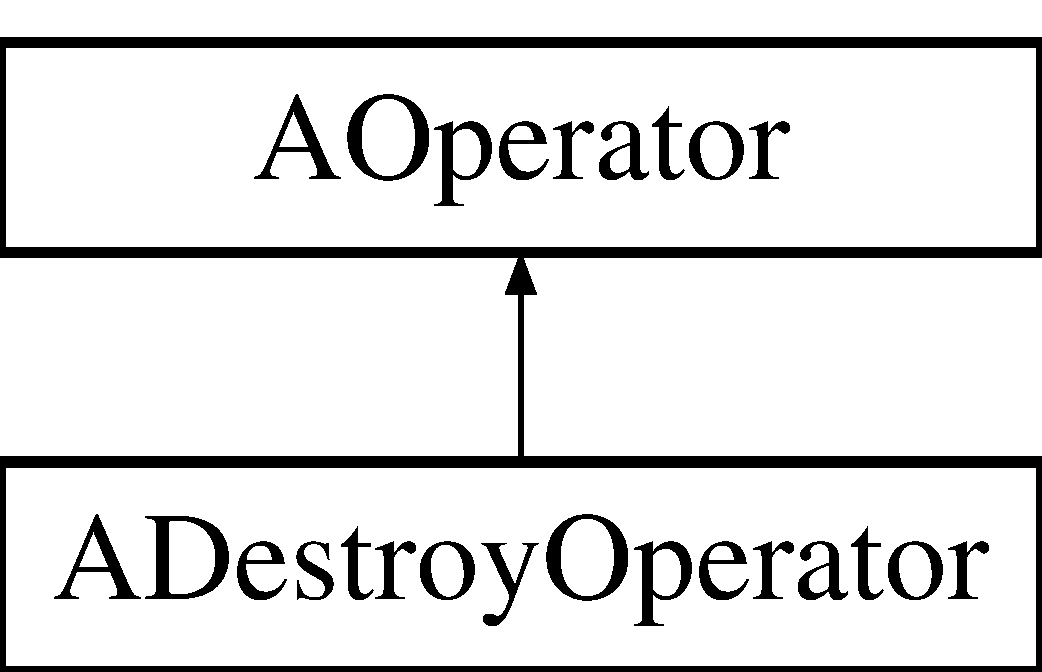
\includegraphics[height=2.000000cm]{classADestroyOperator}
\end{center}
\end{figure}
\subsection*{Public Member Functions}
\begin{DoxyCompactItemize}
\item 
\hyperlink{classADestroyOperator_a95d52552857dc3cdb076513b27a7fa0e}{A\-Destroy\-Operator} (size\-\_\-t mini, size\-\_\-t maxi, std\-::string s)
\item 
\hypertarget{classADestroyOperator_a03fcb4d2756e265417956981062b1c63}{virtual \hyperlink{classADestroyOperator_a03fcb4d2756e265417956981062b1c63}{$\sim$\-A\-Destroy\-Operator} ()}\label{classADestroyOperator_a03fcb4d2756e265417956981062b1c63}

\begin{DoxyCompactList}\small\item\em Destructor. \end{DoxyCompactList}\item 
virtual void \hyperlink{classADestroyOperator_a3a744fb78222835cd4d9cf20bd4ffdb7}{destroy\-Solution} (\hyperlink{classISolution}{I\-Solution} \&sol)=0
\end{DoxyCompactItemize}
\subsection*{Protected Attributes}
\begin{DoxyCompactItemize}
\item 
\hypertarget{classADestroyOperator_a966017d5974080bade3385ccf805bf52}{size\-\_\-t \hyperlink{classADestroyOperator_a966017d5974080bade3385ccf805bf52}{minimun\-Destroy}}\label{classADestroyOperator_a966017d5974080bade3385ccf805bf52}

\begin{DoxyCompactList}\small\item\em The minimum destroy size used. \end{DoxyCompactList}\item 
\hypertarget{classADestroyOperator_a5b5ab82e3407c05cf1ff1d90c0e31905}{size\-\_\-t \hyperlink{classADestroyOperator_a5b5ab82e3407c05cf1ff1d90c0e31905}{maximum\-Destroy}}\label{classADestroyOperator_a5b5ab82e3407c05cf1ff1d90c0e31905}

\begin{DoxyCompactList}\small\item\em The maximum destroy size used. \end{DoxyCompactList}\end{DoxyCompactItemize}


\subsection{Detailed Description}
This is an abstract class used to represent Destroy Operators. 

Any destroy operator should inherit from this class and implement the destroy\-Solution function. 

\subsection{Constructor \& Destructor Documentation}
\hypertarget{classADestroyOperator_a95d52552857dc3cdb076513b27a7fa0e}{\index{A\-Destroy\-Operator@{A\-Destroy\-Operator}!A\-Destroy\-Operator@{A\-Destroy\-Operator}}
\index{A\-Destroy\-Operator@{A\-Destroy\-Operator}!ADestroyOperator@{A\-Destroy\-Operator}}
\subsubsection[{A\-Destroy\-Operator}]{\setlength{\rightskip}{0pt plus 5cm}A\-Destroy\-Operator\-::\-A\-Destroy\-Operator (
\begin{DoxyParamCaption}
\item[{size\-\_\-t}]{mini, }
\item[{size\-\_\-t}]{maxi, }
\item[{std\-::string}]{s}
\end{DoxyParamCaption}
)\hspace{0.3cm}{\ttfamily [inline]}}}\label{classADestroyOperator_a95d52552857dc3cdb076513b27a7fa0e}
Constructor. 
\begin{DoxyParams}{Parameters}
{\em mini} & the minimum destroy size. \\
\hline
{\em maxi} & the maximum destroy size. \\
\hline
{\em s} & the name of the destroy operator. \\
\hline
\end{DoxyParams}


\subsection{Member Function Documentation}
\hypertarget{classADestroyOperator_a3a744fb78222835cd4d9cf20bd4ffdb7}{\index{A\-Destroy\-Operator@{A\-Destroy\-Operator}!destroy\-Solution@{destroy\-Solution}}
\index{destroy\-Solution@{destroy\-Solution}!ADestroyOperator@{A\-Destroy\-Operator}}
\subsubsection[{destroy\-Solution}]{\setlength{\rightskip}{0pt plus 5cm}virtual void A\-Destroy\-Operator\-::destroy\-Solution (
\begin{DoxyParamCaption}
\item[{{\bf I\-Solution} \&}]{sol}
\end{DoxyParamCaption}
)\hspace{0.3cm}{\ttfamily [pure virtual]}}}\label{classADestroyOperator_a3a744fb78222835cd4d9cf20bd4ffdb7}
This function is the one called to destroy a solution. 
\begin{DoxyParams}{Parameters}
{\em sol} & the solution to be destroyed. \\
\hline
\end{DoxyParams}


The documentation for this class was generated from the following file\-:\begin{DoxyCompactItemize}
\item 
src/alns/A\-Destroy\-Operator.\-h\end{DoxyCompactItemize}

\hypertarget{classALNS}{\section{A\-L\-N\-S Class Reference}
\label{classALNS}\index{A\-L\-N\-S@{A\-L\-N\-S}}
}


This class contains the \hyperlink{classALNS}{A\-L\-N\-S} logic.  




{\ttfamily \#include $<$A\-L\-N\-S.\-h$>$}

\subsection*{Public Member Functions}
\begin{DoxyCompactItemize}
\item 
\hyperlink{classALNS_a73b1c0d89a08733cf96b8bd3bd3b1ee0}{A\-L\-N\-S} (std\-::string instance\-Name, \hyperlink{classISolution}{I\-Solution} \&initial\-Solution, \hyperlink{classIAcceptanceModule}{I\-Acceptance\-Module} \&acceptance\-Crit, \hyperlink{classALNS__Parameters}{A\-L\-N\-S\-\_\-\-Parameters} \&parameters, \hyperlink{classAOperatorManager}{A\-Operator\-Manager} \&op\-Man, \hyperlink{classIBestSolutionManager}{I\-Best\-Solution\-Manager} \&sol\-Man, \hyperlink{classILocalSearchManager}{I\-Local\-Search\-Manager} \&ls\-Man)
\item 
\hypertarget{classALNS_a981532332c893575df882950ba108420}{virtual \hyperlink{classALNS_a981532332c893575df882950ba108420}{$\sim$\-A\-L\-N\-S} ()}\label{classALNS_a981532332c893575df882950ba108420}

\begin{DoxyCompactList}\small\item\em Destructor. \end{DoxyCompactList}\item 
bool \hyperlink{classALNS_a02bfc43130ca878023ab85da3990aee8}{solve} ()
\item 
bool \hyperlink{classALNS_a603d6dfef21bcb16cb0d4e0ee70dcad8}{check\-Against\-Known\-Solution} (\hyperlink{classISolution}{I\-Solution} \&sol)
\item 
void \hyperlink{classALNS_af86fb8b68cd36fc947c53d53edf37841}{perform\-One\-Iteration} ()
\item 
\hypertarget{classALNS_a914ea0dff7f09b5fd5da9ab8040515a7}{bool \hyperlink{classALNS_a914ea0dff7f09b5fd5da9ab8040515a7}{is\-Stopping\-Criterion\-Met} ()}\label{classALNS_a914ea0dff7f09b5fd5da9ab8040515a7}

\begin{DoxyCompactList}\small\item\em This method check whether or not the stopping criteria is met. \end{DoxyCompactList}\item 
bool \hyperlink{classALNS_a3dec1742b0f3e6bfc03a087ccb1cf5ee}{is\-New\-Best} (\hyperlink{classISolution}{I\-Solution} $\ast$new\-Sol)
\item 
size\-\_\-t \hyperlink{classALNS_a24567f634de0dd28dc09c7ccde13f7c2}{get\-Number\-Known\-Solutions} ()
\item 
bool \hyperlink{classALNS_a6c9c4ccbbfac3a70ef92dca8fbff68b4}{transition\-Current\-Solution} (\hyperlink{classISolution}{I\-Solution} $\ast$new\-Sol)
\item 
\hypertarget{classALNS_a8070a2581e7cee3cb46452eef5f97aaf}{\hyperlink{classIBestSolutionManager}{I\-Best\-Solution\-Manager} $\ast$ \hyperlink{classALNS_a8070a2581e7cee3cb46452eef5f97aaf}{get\-Best\-Solution\-Manager} ()}\label{classALNS_a8070a2581e7cee3cb46452eef5f97aaf}

\begin{DoxyCompactList}\small\item\em Return a pointer to the best known solution. \end{DoxyCompactList}\item 
void \hyperlink{classALNS_adde152b15ac1197b1b31232ee205072c}{add\-Updatable} (\hyperlink{classIUpdatable}{I\-Updatable} \&up)
\item 
void \hyperlink{classALNS_a6d32f5f1178d89d4f34fc19aff270a5b}{end} ()
\end{DoxyCompactItemize}


\subsection{Detailed Description}
This class contains the \hyperlink{classALNS}{A\-L\-N\-S} logic. 

This class contains the logic of the \hyperlink{classALNS}{A\-L\-N\-S} (Adaptive Large Neighborhood Search). The general idea of the \hyperlink{classALNS}{A\-L\-N\-S} is to iteratively destroy then repair a solution to improve its quality. Non improving solution may be accepted as the new current solution according to some acceptance criteria. If you are interested about the general functionning of this method please refer to\-: S. Ropke \& D. Pisinger. An Adaptive Large Neighborhood Search Heuristic for Pickup and Delivery Problem with Time Windows. Transportation Science, 40 (2006) 455-\/472. 

\subsection{Constructor \& Destructor Documentation}
\hypertarget{classALNS_a73b1c0d89a08733cf96b8bd3bd3b1ee0}{\index{A\-L\-N\-S@{A\-L\-N\-S}!A\-L\-N\-S@{A\-L\-N\-S}}
\index{A\-L\-N\-S@{A\-L\-N\-S}!ALNS@{A\-L\-N\-S}}
\subsubsection[{A\-L\-N\-S}]{\setlength{\rightskip}{0pt plus 5cm}A\-L\-N\-S\-::\-A\-L\-N\-S (
\begin{DoxyParamCaption}
\item[{std\-::string}]{instance\-Name, }
\item[{{\bf I\-Solution} \&}]{initial\-Solution, }
\item[{{\bf I\-Acceptance\-Module} \&}]{acceptance\-Crit, }
\item[{{\bf A\-L\-N\-S\-\_\-\-Parameters} \&}]{parameters, }
\item[{{\bf A\-Operator\-Manager} \&}]{op\-Man, }
\item[{{\bf I\-Best\-Solution\-Manager} \&}]{sol\-Man, }
\item[{{\bf I\-Local\-Search\-Manager} \&}]{ls\-Man}
\end{DoxyParamCaption}
)}}\label{classALNS_a73b1c0d89a08733cf96b8bd3bd3b1ee0}
Constructor. 
\begin{DoxyParams}{Parameters}
{\em name} & the name of the instance. \\
\hline
{\em initial\-Solution} & the starting solution that is going to be optimized. \\
\hline
{\em acceptance\-Crit} & the module that determine whether or not a new solution is accepted as the current solution. \\
\hline
{\em parameters} & the set of parameters to be use by the \hyperlink{classALNS}{A\-L\-N\-S}. \\
\hline
{\em op\-Man} & an operator manager. \\
\hline
\end{DoxyParams}


\subsection{Member Function Documentation}
\hypertarget{classALNS_adde152b15ac1197b1b31232ee205072c}{\index{A\-L\-N\-S@{A\-L\-N\-S}!add\-Updatable@{add\-Updatable}}
\index{add\-Updatable@{add\-Updatable}!ALNS@{A\-L\-N\-S}}
\subsubsection[{add\-Updatable}]{\setlength{\rightskip}{0pt plus 5cm}void A\-L\-N\-S\-::add\-Updatable (
\begin{DoxyParamCaption}
\item[{{\bf I\-Updatable} \&}]{up}
\end{DoxyParamCaption}
)\hspace{0.3cm}{\ttfamily [inline]}}}\label{classALNS_adde152b15ac1197b1b31232ee205072c}
Add an object to the list of object to be updated at the end of each iteration of the \hyperlink{classALNS}{A\-L\-N\-S}. 
\begin{DoxyParams}{Parameters}
{\em up} & the updatable object to be added. \\
\hline
\end{DoxyParams}
\hypertarget{classALNS_a603d6dfef21bcb16cb0d4e0ee70dcad8}{\index{A\-L\-N\-S@{A\-L\-N\-S}!check\-Against\-Known\-Solution@{check\-Against\-Known\-Solution}}
\index{check\-Against\-Known\-Solution@{check\-Against\-Known\-Solution}!ALNS@{A\-L\-N\-S}}
\subsubsection[{check\-Against\-Known\-Solution}]{\setlength{\rightskip}{0pt plus 5cm}bool A\-L\-N\-S\-::check\-Against\-Known\-Solution (
\begin{DoxyParamCaption}
\item[{{\bf I\-Solution} \&}]{sol}
\end{DoxyParamCaption}
)}}\label{classALNS_a603d6dfef21bcb16cb0d4e0ee70dcad8}
This method seeks if a solution is already known, if not it is added to the set of known solutions. 
\begin{DoxyParams}{Parameters}
{\em sol} & the solution to be checked. \\
\hline
\end{DoxyParams}
\begin{DoxyReturn}{Returns}
true if the solution was unknown, false otherwise. 
\end{DoxyReturn}
\hypertarget{classALNS_a6d32f5f1178d89d4f34fc19aff270a5b}{\index{A\-L\-N\-S@{A\-L\-N\-S}!end@{end}}
\index{end@{end}!ALNS@{A\-L\-N\-S}}
\subsubsection[{end}]{\setlength{\rightskip}{0pt plus 5cm}void A\-L\-N\-S\-::end (
\begin{DoxyParamCaption}
{}
\end{DoxyParamCaption}
)}}\label{classALNS_a6d32f5f1178d89d4f34fc19aff270a5b}
Destroy the manager that have been provided at the construction of the instance. \hypertarget{classALNS_a24567f634de0dd28dc09c7ccde13f7c2}{\index{A\-L\-N\-S@{A\-L\-N\-S}!get\-Number\-Known\-Solutions@{get\-Number\-Known\-Solutions}}
\index{get\-Number\-Known\-Solutions@{get\-Number\-Known\-Solutions}!ALNS@{A\-L\-N\-S}}
\subsubsection[{get\-Number\-Known\-Solutions}]{\setlength{\rightskip}{0pt plus 5cm}size\-\_\-t A\-L\-N\-S\-::get\-Number\-Known\-Solutions (
\begin{DoxyParamCaption}
{}
\end{DoxyParamCaption}
)\hspace{0.3cm}{\ttfamily [inline]}}}\label{classALNS_a24567f634de0dd28dc09c7ccde13f7c2}
\begin{DoxyReturn}{Returns}
the number of known solutions. 
\end{DoxyReturn}
\hypertarget{classALNS_a3dec1742b0f3e6bfc03a087ccb1cf5ee}{\index{A\-L\-N\-S@{A\-L\-N\-S}!is\-New\-Best@{is\-New\-Best}}
\index{is\-New\-Best@{is\-New\-Best}!ALNS@{A\-L\-N\-S}}
\subsubsection[{is\-New\-Best}]{\setlength{\rightskip}{0pt plus 5cm}bool A\-L\-N\-S\-::is\-New\-Best (
\begin{DoxyParamCaption}
\item[{{\bf I\-Solution} $\ast$}]{new\-Sol}
\end{DoxyParamCaption}
)}}\label{classALNS_a3dec1742b0f3e6bfc03a087ccb1cf5ee}
Determine whether or not the new solution is better than the best known solution. \hypertarget{classALNS_af86fb8b68cd36fc947c53d53edf37841}{\index{A\-L\-N\-S@{A\-L\-N\-S}!perform\-One\-Iteration@{perform\-One\-Iteration}}
\index{perform\-One\-Iteration@{perform\-One\-Iteration}!ALNS@{A\-L\-N\-S}}
\subsubsection[{perform\-One\-Iteration}]{\setlength{\rightskip}{0pt plus 5cm}void A\-L\-N\-S\-::perform\-One\-Iteration (
\begin{DoxyParamCaption}
{}
\end{DoxyParamCaption}
)}}\label{classALNS_af86fb8b68cd36fc947c53d53edf37841}
This method perform one iteration of the \hyperlink{classALNS}{A\-L\-N\-S} solving process. \hypertarget{classALNS_a02bfc43130ca878023ab85da3990aee8}{\index{A\-L\-N\-S@{A\-L\-N\-S}!solve@{solve}}
\index{solve@{solve}!ALNS@{A\-L\-N\-S}}
\subsubsection[{solve}]{\setlength{\rightskip}{0pt plus 5cm}bool A\-L\-N\-S\-::solve (
\begin{DoxyParamCaption}
{}
\end{DoxyParamCaption}
)}}\label{classALNS_a02bfc43130ca878023ab85da3990aee8}
This method launch the solving process. \begin{DoxyReturn}{Returns}
true if a feasible solution is found, false otherwise. 
\end{DoxyReturn}
\hypertarget{classALNS_a6c9c4ccbbfac3a70ef92dca8fbff68b4}{\index{A\-L\-N\-S@{A\-L\-N\-S}!transition\-Current\-Solution@{transition\-Current\-Solution}}
\index{transition\-Current\-Solution@{transition\-Current\-Solution}!ALNS@{A\-L\-N\-S}}
\subsubsection[{transition\-Current\-Solution}]{\setlength{\rightskip}{0pt plus 5cm}bool A\-L\-N\-S\-::transition\-Current\-Solution (
\begin{DoxyParamCaption}
\item[{{\bf I\-Solution} $\ast$}]{new\-Sol}
\end{DoxyParamCaption}
)}}\label{classALNS_a6c9c4ccbbfac3a70ef92dca8fbff68b4}
Determine whether or not the new solution should be accepted as the current solution. 

The documentation for this class was generated from the following files\-:\begin{DoxyCompactItemize}
\item 
src/alns/A\-L\-N\-S.\-h\item 
src/alns/A\-L\-N\-S.\-cpp\end{DoxyCompactItemize}

\hypertarget{classALNS__Iteration__Status}{\section{A\-L\-N\-S\-\_\-\-Iteration\-\_\-\-Status Class Reference}
\label{classALNS__Iteration__Status}\index{A\-L\-N\-S\-\_\-\-Iteration\-\_\-\-Status@{A\-L\-N\-S\-\_\-\-Iteration\-\_\-\-Status}}
}


This class represent the output of an iteration of the \hyperlink{classALNS}{A\-L\-N\-S}.  




{\ttfamily \#include $<$A\-L\-N\-S\-\_\-\-Iteration\-\_\-\-Status.\-h$>$}

\subsection*{Public Types}
\begin{DoxyCompactItemize}
\item 
enum \hyperlink{classALNS__Iteration__Status_a6d748b05080edeab9e82ac32c9904133}{State} \{ {\bfseries T\-R\-U\-E}, 
{\bfseries F\-A\-L\-S\-E}, 
{\bfseries U\-N\-K\-N\-O\-W\-N}
 \}
\begin{DoxyCompactList}\small\item\em An enumeration representing a boolean with an unknown state. \end{DoxyCompactList}\end{DoxyCompactItemize}
\subsection*{Public Member Functions}
\begin{DoxyCompactItemize}
\item 
\hypertarget{classALNS__Iteration__Status_acc9ee7e67246f657659962c38042884b}{\hyperlink{classALNS__Iteration__Status_acc9ee7e67246f657659962c38042884b}{A\-L\-N\-S\-\_\-\-Iteration\-\_\-\-Status} ()}\label{classALNS__Iteration__Status_acc9ee7e67246f657659962c38042884b}

\begin{DoxyCompactList}\small\item\em Constructor. \end{DoxyCompactList}\item 
\hypertarget{classALNS__Iteration__Status_a27b79dc877bc9215b37c418ec92e2b72}{void \hyperlink{classALNS__Iteration__Status_a27b79dc877bc9215b37c418ec92e2b72}{partial\-Reinit} ()}\label{classALNS__Iteration__Status_a27b79dc877bc9215b37c418ec92e2b72}

\begin{DoxyCompactList}\small\item\em Reinitialize some values. \end{DoxyCompactList}\item 
\hypertarget{classALNS__Iteration__Status_a23e9feb28251b9c1021a1f38412620d0}{\hyperlink{classALNS__Iteration__Status_a6d748b05080edeab9e82ac32c9904133}{State} \hyperlink{classALNS__Iteration__Status_a23e9feb28251b9c1021a1f38412620d0}{get\-Accepted\-As\-Current\-Solution} () const }\label{classALNS__Iteration__Status_a23e9feb28251b9c1021a1f38412620d0}

\begin{DoxyCompactList}\small\item\em Simple getter. \end{DoxyCompactList}\item 
\hypertarget{classALNS__Iteration__Status_a61328f04761ab800faeeac7ecbdfd237}{\hyperlink{classALNS__Iteration__Status_a6d748b05080edeab9e82ac32c9904133}{State} \hyperlink{classALNS__Iteration__Status_a61328f04761ab800faeeac7ecbdfd237}{get\-Already\-Known\-Solution} () const }\label{classALNS__Iteration__Status_a61328f04761ab800faeeac7ecbdfd237}

\begin{DoxyCompactList}\small\item\em Simple getter. \end{DoxyCompactList}\item 
\hypertarget{classALNS__Iteration__Status_a2eaccbb6eefebbdf5f6f2031570857b5}{\hyperlink{classALNS__Iteration__Status_a6d748b05080edeab9e82ac32c9904133}{State} \hyperlink{classALNS__Iteration__Status_a2eaccbb6eefebbdf5f6f2031570857b5}{get\-Improve\-Current\-Solution} () const }\label{classALNS__Iteration__Status_a2eaccbb6eefebbdf5f6f2031570857b5}

\begin{DoxyCompactList}\small\item\em Simple getter. \end{DoxyCompactList}\item 
\hypertarget{classALNS__Iteration__Status_a88178a99b0c70ed6bba29f3ca3422263}{size\-\_\-t \hyperlink{classALNS__Iteration__Status_a88178a99b0c70ed6bba29f3ca3422263}{get\-Iteration\-Id} () const }\label{classALNS__Iteration__Status_a88178a99b0c70ed6bba29f3ca3422263}

\begin{DoxyCompactList}\small\item\em Simple getter. \end{DoxyCompactList}\item 
\hypertarget{classALNS__Iteration__Status_aaa6f6deb1a2eef0c5fbaf501633c0fa4}{size\-\_\-t \hyperlink{classALNS__Iteration__Status_aaa6f6deb1a2eef0c5fbaf501633c0fa4}{get\-Nb\-Iteration\-Without\-Improvement} () const }\label{classALNS__Iteration__Status_aaa6f6deb1a2eef0c5fbaf501633c0fa4}

\begin{DoxyCompactList}\small\item\em Simple getter. \end{DoxyCompactList}\item 
\hypertarget{classALNS__Iteration__Status_ad67a5c238a0dcc071eb596fed5db91d1}{size\-\_\-t \hyperlink{classALNS__Iteration__Status_ad67a5c238a0dcc071eb596fed5db91d1}{get\-Nb\-Iteration\-Without\-Improvement\-Current} () const }\label{classALNS__Iteration__Status_ad67a5c238a0dcc071eb596fed5db91d1}

\begin{DoxyCompactList}\small\item\em Simple getter. \end{DoxyCompactList}\item 
\hypertarget{classALNS__Iteration__Status_a676ecc31ff5d41df003cb5883e120e4b}{size\-\_\-t \hyperlink{classALNS__Iteration__Status_a676ecc31ff5d41df003cb5883e120e4b}{get\-Nb\-Iteration\-Without\-Transition} () const }\label{classALNS__Iteration__Status_a676ecc31ff5d41df003cb5883e120e4b}

\begin{DoxyCompactList}\small\item\em Simple getter. \end{DoxyCompactList}\item 
\hypertarget{classALNS__Iteration__Status_a36a461656092c00b578b380b19a31d2a}{\hyperlink{classALNS__Iteration__Status_a6d748b05080edeab9e82ac32c9904133}{State} \hyperlink{classALNS__Iteration__Status_a36a461656092c00b578b380b19a31d2a}{get\-New\-Best\-Solution} () const }\label{classALNS__Iteration__Status_a36a461656092c00b578b380b19a31d2a}

\begin{DoxyCompactList}\small\item\em Simple getter. \end{DoxyCompactList}\item 
\hypertarget{classALNS__Iteration__Status_a9b9cc03cf195a9079704d4675e0b78aa}{void \hyperlink{classALNS__Iteration__Status_a9b9cc03cf195a9079704d4675e0b78aa}{set\-Accepted\-As\-Current\-Solution} (\hyperlink{classALNS__Iteration__Status_a6d748b05080edeab9e82ac32c9904133}{State} accepted\-As\-Current\-Solution)}\label{classALNS__Iteration__Status_a9b9cc03cf195a9079704d4675e0b78aa}

\begin{DoxyCompactList}\small\item\em Simple setter. \end{DoxyCompactList}\item 
\hypertarget{classALNS__Iteration__Status_ac8c5a5db9230c5a55c971ee11abced9a}{void \hyperlink{classALNS__Iteration__Status_ac8c5a5db9230c5a55c971ee11abced9a}{set\-Already\-Known\-Solution} (\hyperlink{classALNS__Iteration__Status_a6d748b05080edeab9e82ac32c9904133}{State} already\-Known\-Solution)}\label{classALNS__Iteration__Status_ac8c5a5db9230c5a55c971ee11abced9a}

\begin{DoxyCompactList}\small\item\em Simple setter. \end{DoxyCompactList}\item 
\hypertarget{classALNS__Iteration__Status_a6ecfed253c531820cf90016753e0a6c1}{void \hyperlink{classALNS__Iteration__Status_a6ecfed253c531820cf90016753e0a6c1}{set\-Improve\-Current\-Solution} (\hyperlink{classALNS__Iteration__Status_a6d748b05080edeab9e82ac32c9904133}{State} improve\-Current\-Solution)}\label{classALNS__Iteration__Status_a6ecfed253c531820cf90016753e0a6c1}

\begin{DoxyCompactList}\small\item\em Simple setter. \end{DoxyCompactList}\item 
\hypertarget{classALNS__Iteration__Status_a0bf1e96a39704e945dc2505bbf6f73ea}{void \hyperlink{classALNS__Iteration__Status_a0bf1e96a39704e945dc2505bbf6f73ea}{set\-Iteration\-Id} (size\-\_\-t iteration\-Id)}\label{classALNS__Iteration__Status_a0bf1e96a39704e945dc2505bbf6f73ea}

\begin{DoxyCompactList}\small\item\em Simple setter. \end{DoxyCompactList}\item 
\hypertarget{classALNS__Iteration__Status_a98c4b0753e01bc625fa43c35e02d47ec}{void \hyperlink{classALNS__Iteration__Status_a98c4b0753e01bc625fa43c35e02d47ec}{set\-Nb\-Iteration\-Without\-Improvement} (size\-\_\-t nb\-Iteration\-Without\-Improvement)}\label{classALNS__Iteration__Status_a98c4b0753e01bc625fa43c35e02d47ec}

\begin{DoxyCompactList}\small\item\em Simple setter. \end{DoxyCompactList}\item 
\hypertarget{classALNS__Iteration__Status_a23d0db24e275cdc792b624b792020491}{void \hyperlink{classALNS__Iteration__Status_a23d0db24e275cdc792b624b792020491}{set\-Nb\-Iteration\-Without\-Improvement\-Current} (size\-\_\-t nb\-Iteration\-Without\-Improvement\-Current)}\label{classALNS__Iteration__Status_a23d0db24e275cdc792b624b792020491}

\begin{DoxyCompactList}\small\item\em Simple setter. \end{DoxyCompactList}\item 
\hypertarget{classALNS__Iteration__Status_ada17bcf0bfcb2f4dfb1fb3a5495e9dd1}{void \hyperlink{classALNS__Iteration__Status_ada17bcf0bfcb2f4dfb1fb3a5495e9dd1}{set\-Nb\-Iteration\-Without\-Transition} (size\-\_\-t nb\-Iteration\-Without\-Transition)}\label{classALNS__Iteration__Status_ada17bcf0bfcb2f4dfb1fb3a5495e9dd1}

\begin{DoxyCompactList}\small\item\em Simple setter. \end{DoxyCompactList}\item 
\hypertarget{classALNS__Iteration__Status_a84c1ffabe1926283b5c74387e1b4c956}{void \hyperlink{classALNS__Iteration__Status_a84c1ffabe1926283b5c74387e1b4c956}{set\-New\-Best\-Solution} (\hyperlink{classALNS__Iteration__Status_a6d748b05080edeab9e82ac32c9904133}{State} new\-Best\-Solution)}\label{classALNS__Iteration__Status_a84c1ffabe1926283b5c74387e1b4c956}

\begin{DoxyCompactList}\small\item\em Simple setter. \end{DoxyCompactList}\item 
\hypertarget{classALNS__Iteration__Status_a0c1f750deed2f1e4291aff01025f5f79}{\hyperlink{classALNS__Iteration__Status_a0c1f750deed2f1e4291aff01025f5f79}{$\sim$\-A\-L\-N\-S\-\_\-\-Iteration\-\_\-\-Status} ()}\label{classALNS__Iteration__Status_a0c1f750deed2f1e4291aff01025f5f79}

\begin{DoxyCompactList}\small\item\em Destructor. \end{DoxyCompactList}\item 
\hypertarget{classALNS__Iteration__Status_aeaece7fc0a46c4e7052dc27cb29e82dc}{\hyperlink{classALNS__Iteration__Status_a6d748b05080edeab9e82ac32c9904133}{State} \hyperlink{classALNS__Iteration__Status_aeaece7fc0a46c4e7052dc27cb29e82dc}{get\-Improve\-By\-Local\-Search} () const }\label{classALNS__Iteration__Status_aeaece7fc0a46c4e7052dc27cb29e82dc}

\begin{DoxyCompactList}\small\item\em Simple getter. \end{DoxyCompactList}\item 
\hypertarget{classALNS__Iteration__Status_adc7244a328e029db2e08d2b033dd26cd}{\hyperlink{classALNS__Iteration__Status_a6d748b05080edeab9e82ac32c9904133}{State} \hyperlink{classALNS__Iteration__Status_adc7244a328e029db2e08d2b033dd26cd}{get\-Local\-Search\-Used} () const }\label{classALNS__Iteration__Status_adc7244a328e029db2e08d2b033dd26cd}

\begin{DoxyCompactList}\small\item\em Simple getter. \end{DoxyCompactList}\item 
\hypertarget{classALNS__Iteration__Status_a702fd3ae594f8c4721a7e4d71269ed2a}{void \hyperlink{classALNS__Iteration__Status_a702fd3ae594f8c4721a7e4d71269ed2a}{set\-Improve\-By\-Local\-Search} (\hyperlink{classALNS__Iteration__Status_a6d748b05080edeab9e82ac32c9904133}{State} improve\-By\-Local\-Search)}\label{classALNS__Iteration__Status_a702fd3ae594f8c4721a7e4d71269ed2a}

\begin{DoxyCompactList}\small\item\em Simple setter. \end{DoxyCompactList}\item 
\hypertarget{classALNS__Iteration__Status_a08a7d8a3d191f49bcbe4ccbe315ca905}{void \hyperlink{classALNS__Iteration__Status_a08a7d8a3d191f49bcbe4ccbe315ca905}{set\-Local\-Search\-Used} (\hyperlink{classALNS__Iteration__Status_a6d748b05080edeab9e82ac32c9904133}{State} local\-Search\-Used)}\label{classALNS__Iteration__Status_a08a7d8a3d191f49bcbe4ccbe315ca905}

\begin{DoxyCompactList}\small\item\em Simple setter. \end{DoxyCompactList}\item 
\hypertarget{classALNS__Iteration__Status_af90d4acaa09495f6fab3c1ae9ed681e3}{size\-\_\-t {\bfseries get\-Nb\-Iteration\-Without\-Improvement\-Since\-Last\-Reload} () const }\label{classALNS__Iteration__Status_af90d4acaa09495f6fab3c1ae9ed681e3}

\item 
\hypertarget{classALNS__Iteration__Status_a4722cfab19d9912dc51ff447a0a3fb99}{void {\bfseries set\-Nb\-Iteration\-Without\-Improvement\-Since\-Last\-Reload} (size\-\_\-t nb)}\label{classALNS__Iteration__Status_a4722cfab19d9912dc51ff447a0a3fb99}

\item 
\hypertarget{classALNS__Iteration__Status_a6683f3e5c476a9387eebd3db2c455e36}{\hyperlink{classALNS__Iteration__Status_a6d748b05080edeab9e82ac32c9904133}{State} {\bfseries get\-Already\-Destroyed} () const }\label{classALNS__Iteration__Status_a6683f3e5c476a9387eebd3db2c455e36}

\item 
\hypertarget{classALNS__Iteration__Status_aa3ea7c59a5c55fd4ec32516e3c4d9d2e}{void {\bfseries set\-Already\-Destroyed} (\hyperlink{classALNS__Iteration__Status_a6d748b05080edeab9e82ac32c9904133}{State} already\-Destroyed)}\label{classALNS__Iteration__Status_aa3ea7c59a5c55fd4ec32516e3c4d9d2e}

\item 
\hypertarget{classALNS__Iteration__Status_a400f479c974f6279124033504b327386}{\hyperlink{classALNS__Iteration__Status_a6d748b05080edeab9e82ac32c9904133}{State} {\bfseries get\-Already\-Repaired} () const }\label{classALNS__Iteration__Status_a400f479c974f6279124033504b327386}

\item 
\hypertarget{classALNS__Iteration__Status_abc814ed1e79192b0454a20fe9c2175cb}{void {\bfseries set\-Already\-Repaired} (\hyperlink{classALNS__Iteration__Status_a6d748b05080edeab9e82ac32c9904133}{State} already\-Repaired)}\label{classALNS__Iteration__Status_abc814ed1e79192b0454a20fe9c2175cb}

\end{DoxyCompactItemize}


\subsection{Detailed Description}
This class represent the output of an iteration of the \hyperlink{classALNS}{A\-L\-N\-S}. 

The documentation for this class was generated from the following file\-:\begin{DoxyCompactItemize}
\item 
src/alns/A\-L\-N\-S\-\_\-\-Iteration\-\_\-\-Status.\-h\end{DoxyCompactItemize}

\hypertarget{classALNS__Parameters}{\section{A\-L\-N\-S\-\_\-\-Parameters Class Reference}
\label{classALNS__Parameters}\index{A\-L\-N\-S\-\_\-\-Parameters@{A\-L\-N\-S\-\_\-\-Parameters}}
}


This class contains parameters to be used by the \hyperlink{classALNS}{A\-L\-N\-S}.  




{\ttfamily \#include $<$A\-L\-N\-S\-\_\-\-Parameters.\-h$>$}

Inheritance diagram for A\-L\-N\-S\-\_\-\-Parameters\-:\begin{figure}[H]
\begin{center}
\leavevmode
\includegraphics[height=2.000000cm]{classALNS__Parameters}
\end{center}
\end{figure}
\subsection*{Public Types}
\begin{DoxyCompactItemize}
\item 
enum \hyperlink{classALNS__Parameters_ae252d050b207dee5b442ca7d02c1d831}{Stopping\-Criteria} \{ {\bfseries M\-A\-X\-\_\-\-I\-T}, 
{\bfseries M\-A\-X\-\_\-\-R\-T}, 
{\bfseries M\-A\-X\-\_\-\-I\-T\-\_\-\-N\-O\-\_\-\-I\-M\-P}, 
{\bfseries A\-L\-L}
 \}
\item 
enum \hyperlink{classALNS__Parameters_addd5421947a7a1a533fec576f37560c7}{Acceptance\-Criterio\-Kind} \{ {\bfseries S\-A}
 \}
\begin{DoxyCompactList}\small\item\em An enumeration listing a set of packaged Acceptance\-Module Implementation. \end{DoxyCompactList}\end{DoxyCompactItemize}
\subsection*{Public Member Functions}
\begin{DoxyCompactItemize}
\item 
\hypertarget{classALNS__Parameters_a361ec5dedae42ac8ef4e15bac35ffc5b}{\hyperlink{classALNS__Parameters_a361ec5dedae42ac8ef4e15bac35ffc5b}{A\-L\-N\-S\-\_\-\-Parameters} ()}\label{classALNS__Parameters_a361ec5dedae42ac8ef4e15bac35ffc5b}

\begin{DoxyCompactList}\small\item\em Constructor. \end{DoxyCompactList}\item 
\hypertarget{classALNS__Parameters_a009eb8cb2d8b5de326cb945592b5f927}{\hyperlink{classALNS__Parameters_a009eb8cb2d8b5de326cb945592b5f927}{A\-L\-N\-S\-\_\-\-Parameters} (\hyperlink{classALNS__Parameters}{A\-L\-N\-S\-\_\-\-Parameters} \&p)}\label{classALNS__Parameters_a009eb8cb2d8b5de326cb945592b5f927}

\begin{DoxyCompactList}\small\item\em Copy constructor. \end{DoxyCompactList}\item 
\hypertarget{classALNS__Parameters_a6862d124475b2a0c24141c233ea70ac8}{\hyperlink{classALNS__Parameters_a6862d124475b2a0c24141c233ea70ac8}{$\sim$\-A\-L\-N\-S\-\_\-\-Parameters} ()}\label{classALNS__Parameters_a6862d124475b2a0c24141c233ea70ac8}

\begin{DoxyCompactList}\small\item\em Destructor. \end{DoxyCompactList}\item 
\hypertarget{classALNS__Parameters_a271ab0a53b41317dad182fdb4f11ac61}{void \hyperlink{classALNS__Parameters_a271ab0a53b41317dad182fdb4f11ac61}{sanity\-Checks} ()}\label{classALNS__Parameters_a271ab0a53b41317dad182fdb4f11ac61}

\begin{DoxyCompactList}\small\item\em This method perform some sanity checks on the value of the parameters. \end{DoxyCompactList}\item 
void \hyperlink{classALNS__Parameters_afdafe8203131ddbea64ae09548de4fa4}{load\-Parameters} (std\-::string path)
\item 
void \hyperlink{classALNS__Parameters_a985158e9df4d28113d8e973d0f8d6870}{load\-X\-M\-L\-Parameters} (std\-::string path)
\item 
\hypertarget{classALNS__Parameters_a9c2b89225ffc40f286b6685fc2dc12cf}{size\-\_\-t {\bfseries get\-Reload\-Frequency} () const }\label{classALNS__Parameters_a9c2b89225ffc40f286b6685fc2dc12cf}

\item 
\hypertarget{classALNS__Parameters_a17080f909df5fe9a43a3e90f0457a687}{void {\bfseries set\-Reload\-Frequency} (size\-\_\-t \hyperlink{classALNS__Parameters_ab3c514956945f29a6dff9a77fd5cb3ea}{reload\-Frequency})}\label{classALNS__Parameters_a17080f909df5fe9a43a3e90f0457a687}

\item 
\hypertarget{classALNS__Parameters_ad4ab7e264fd9df231a60cef52bd7774c}{std\-::vector$<$ std\-::string $>$ \hyperlink{classALNS__Parameters_ad4ab7e264fd9df231a60cef52bd7774c}{get\-Forbiden\-Ls\-Operators} () const }\label{classALNS__Parameters_ad4ab7e264fd9df231a60cef52bd7774c}

\begin{DoxyCompactList}\small\item\em Simple getter. \end{DoxyCompactList}\item 
\hypertarget{classALNS__Parameters_a9111acfa9c48a7e6e969bfd4c4908dfb}{void {\bfseries add\-Forbidden\-Ls\-Operator} (std\-::string ls\-Op)}\label{classALNS__Parameters_a9111acfa9c48a7e6e969bfd4c4908dfb}

\item 
\hypertarget{classALNS__Parameters_a609ef48dbcc7b36f2a41ffd8a3a68773}{std\-::vector$<$ std\-::string $>$ \hyperlink{classALNS__Parameters_a609ef48dbcc7b36f2a41ffd8a3a68773}{get\-Forbiden\-Operators} () const }\label{classALNS__Parameters_a609ef48dbcc7b36f2a41ffd8a3a68773}

\begin{DoxyCompactList}\small\item\em Simple getter. \end{DoxyCompactList}\item 
\hypertarget{classALNS__Parameters_a2d81a91ccf46ce1105f05ceb871e206e}{void {\bfseries add\-Forbidden\-Operator} (std\-::string op)}\label{classALNS__Parameters_a2d81a91ccf46ce1105f05ceb871e206e}

\item 
\hypertarget{classALNS__Parameters_a722eae2be52681671ca6ca9b6b6c2461}{bool {\bfseries get\-Perform\-Local\-Search} () const }\label{classALNS__Parameters_a722eae2be52681671ca6ca9b6b6c2461}

\item 
\hypertarget{classALNS__Parameters_aed8815933e774abd40be41620650ecc6}{void {\bfseries set\-Perform\-Local\-Search} (bool \hyperlink{classALNS__Parameters_a6b65081dc41bf2657da46ad28f4a9b23}{perform\-Local\-Search})}\label{classALNS__Parameters_aed8815933e774abd40be41620650ecc6}

\item 
\hypertarget{classALNS__Parameters_a509963d73b2fabb6f32c764221f3aedb}{int {\bfseries get\-Log\-Frequency} () const }\label{classALNS__Parameters_a509963d73b2fabb6f32c764221f3aedb}

\item 
\hypertarget{classALNS__Parameters_a4b25996c01af3f43fba4398ea83840df}{void {\bfseries set\-Log\-Frequency} (int \hyperlink{classALNS__Parameters_ab69fe5b1f01e70f07884185cae0f7805}{log\-Frequency})}\label{classALNS__Parameters_a4b25996c01af3f43fba4398ea83840df}

\item 
\hypertarget{classALNS__Parameters_a4fdc445e48a245e6b6b7cc54606cd3aa}{std\-::string {\bfseries get\-Stats\-Glob\-Path} () const }\label{classALNS__Parameters_a4fdc445e48a245e6b6b7cc54606cd3aa}

\item 
\hypertarget{classALNS__Parameters_a456ab096870f7940f3d0e64f8b4dc737}{std\-::string {\bfseries get\-Stats\-Op\-Path} () const }\label{classALNS__Parameters_a456ab096870f7940f3d0e64f8b4dc737}

\item 
\hypertarget{classALNS__Parameters_aa775aaea00129a37c739c310df88f597}{void {\bfseries set\-Stats\-Glob\-Path} (std\-::string \hyperlink{classALNS__Parameters_a040ee77338cb0393104caf1180ecb498}{stats\-Glob\-Path})}\label{classALNS__Parameters_aa775aaea00129a37c739c310df88f597}

\item 
\hypertarget{classALNS__Parameters_a27e50f68b1bc867d1448827bbc6f585f}{void {\bfseries set\-Stats\-Op\-Path} (std\-::string \hyperlink{classALNS__Parameters_aac994b9eab5d4da5059f6b122160f0c9}{stats\-Op\-Path})}\label{classALNS__Parameters_a27e50f68b1bc867d1448827bbc6f585f}

\item 
\hypertarget{classALNS__Parameters_a39916085f7ead675bb402f0639d29706}{\hyperlink{classALNS__Parameters_addd5421947a7a1a533fec576f37560c7}{Acceptance\-Criterio\-Kind} \hyperlink{classALNS__Parameters_a39916085f7ead675bb402f0639d29706}{get\-Ac\-Kind} () const }\label{classALNS__Parameters_a39916085f7ead675bb402f0639d29706}

\begin{DoxyCompactList}\small\item\em Simple getter. \end{DoxyCompactList}\item 
\hypertarget{classALNS__Parameters_a561e7fb4990b951a6cae7645e70a0091}{std\-::string \hyperlink{classALNS__Parameters_a561e7fb4990b951a6cae7645e70a0091}{get\-Ac\-Path} () const }\label{classALNS__Parameters_a561e7fb4990b951a6cae7645e70a0091}

\begin{DoxyCompactList}\small\item\em Simple getter. \end{DoxyCompactList}\item 
\hypertarget{classALNS__Parameters_a6461ccc2cc454ac777f6ea96f75ee6b3}{void \hyperlink{classALNS__Parameters_a6461ccc2cc454ac777f6ea96f75ee6b3}{set\-Ac\-Kind} (\hyperlink{classALNS__Parameters_addd5421947a7a1a533fec576f37560c7}{Acceptance\-Criterio\-Kind} \hyperlink{classALNS__Parameters_ac87749e7f117607ca350422f6053303f}{ac\-Kind})}\label{classALNS__Parameters_a6461ccc2cc454ac777f6ea96f75ee6b3}

\begin{DoxyCompactList}\small\item\em Simple getter. \end{DoxyCompactList}\item 
\hypertarget{classALNS__Parameters_a2a9425018145a6286424bb69b6e0fc78}{void \hyperlink{classALNS__Parameters_a2a9425018145a6286424bb69b6e0fc78}{set\-Ac\-Path} (std\-::string \hyperlink{classALNS__Parameters_aa5ec5bd7cd255c818888969a1711605e}{ac\-Path})}\label{classALNS__Parameters_a2a9425018145a6286424bb69b6e0fc78}

\begin{DoxyCompactList}\small\item\em Simple getter. \end{DoxyCompactList}\item 
\hypertarget{classALNS__Parameters_a4733612b400549d2ff4a9b3a0280ba3c}{double \hyperlink{classALNS__Parameters_a4733612b400549d2ff4a9b3a0280ba3c}{get\-Probability\-Of\-Noise} () const }\label{classALNS__Parameters_a4733612b400549d2ff4a9b3a0280ba3c}

\begin{DoxyCompactList}\small\item\em Simple getter. \end{DoxyCompactList}\item 
\hypertarget{classALNS__Parameters_a17f2954f75c8bc57ac3ec1716f6346af}{void \hyperlink{classALNS__Parameters_a17f2954f75c8bc57ac3ec1716f6346af}{set\-Probability\-Of\-Noise} (double \hyperlink{classALNS__Parameters_ade0d6fac20ee1d90c5a5a4e0f2f3ac5a}{probability\-Of\-Noise})}\label{classALNS__Parameters_a17f2954f75c8bc57ac3ec1716f6346af}

\begin{DoxyCompactList}\small\item\em Simple getter. \end{DoxyCompactList}\item 
\hypertarget{classALNS__Parameters_a8982fc2669224f8c2bfa14e2ad5a886b}{size\-\_\-t \hyperlink{classALNS__Parameters_a8982fc2669224f8c2bfa14e2ad5a886b}{get\-Max\-Nb\-Iterations} () const }\label{classALNS__Parameters_a8982fc2669224f8c2bfa14e2ad5a886b}

\begin{DoxyCompactList}\small\item\em Simple getter. \end{DoxyCompactList}\item 
\hypertarget{classALNS__Parameters_aa5a042b55fe115f41bebdf99df460ee5}{size\-\_\-t \hyperlink{classALNS__Parameters_aa5a042b55fe115f41bebdf99df460ee5}{get\-Max\-Nb\-Iterations\-No\-Imp} () const }\label{classALNS__Parameters_aa5a042b55fe115f41bebdf99df460ee5}

\begin{DoxyCompactList}\small\item\em Simple getter. \end{DoxyCompactList}\item 
\hypertarget{classALNS__Parameters_a1a81595127071d072e30e0ea02ed3abc}{double \hyperlink{classALNS__Parameters_a1a81595127071d072e30e0ea02ed3abc}{get\-Max\-Running\-Time} () const }\label{classALNS__Parameters_a1a81595127071d072e30e0ea02ed3abc}

\begin{DoxyCompactList}\small\item\em Simple getter. \end{DoxyCompactList}\item 
\hypertarget{classALNS__Parameters_a4a4f411b74c916a981086827eb069ec1}{double \hyperlink{classALNS__Parameters_a4a4f411b74c916a981086827eb069ec1}{get\-Maximum\-Weight} () const }\label{classALNS__Parameters_a4a4f411b74c916a981086827eb069ec1}

\begin{DoxyCompactList}\small\item\em Simple getter. \end{DoxyCompactList}\item 
\hypertarget{classALNS__Parameters_a8519a3e48552b3712e1f070e3a431daf}{double \hyperlink{classALNS__Parameters_a8519a3e48552b3712e1f070e3a431daf}{get\-Minimum\-Weight} () const }\label{classALNS__Parameters_a8519a3e48552b3712e1f070e3a431daf}

\begin{DoxyCompactList}\small\item\em Simple getter. \end{DoxyCompactList}\item 
\hypertarget{classALNS__Parameters_aef0a553ad9753726a122a8e50b36e44e}{size\-\_\-t \hyperlink{classALNS__Parameters_aef0a553ad9753726a122a8e50b36e44e}{get\-Nb\-It\-Before\-Reinit} () const }\label{classALNS__Parameters_aef0a553ad9753726a122a8e50b36e44e}

\begin{DoxyCompactList}\small\item\em Simple getter. \end{DoxyCompactList}\item 
\hypertarget{classALNS__Parameters_a46691475e460589e5d693490a73378bb}{bool \hyperlink{classALNS__Parameters_a46691475e460589e5d693490a73378bb}{get\-Noise} () const }\label{classALNS__Parameters_a46691475e460589e5d693490a73378bb}

\begin{DoxyCompactList}\small\item\em Simple getter. \end{DoxyCompactList}\item 
\hypertarget{classALNS__Parameters_a0bea7982f694c83ed2cee6de78ceeec4}{double \hyperlink{classALNS__Parameters_a0bea7982f694c83ed2cee6de78ceeec4}{get\-Rho} () const }\label{classALNS__Parameters_a0bea7982f694c83ed2cee6de78ceeec4}

\begin{DoxyCompactList}\small\item\em Simple getter. \end{DoxyCompactList}\item 
\hypertarget{classALNS__Parameters_a4da5809a1d38e2f21f4a739eb362e1af}{int \hyperlink{classALNS__Parameters_a4da5809a1d38e2f21f4a739eb362e1af}{get\-Sigma1} () const }\label{classALNS__Parameters_a4da5809a1d38e2f21f4a739eb362e1af}

\begin{DoxyCompactList}\small\item\em Simple getter. \end{DoxyCompactList}\item 
\hypertarget{classALNS__Parameters_a98c62565861d1d5d50079f481753e23f}{int \hyperlink{classALNS__Parameters_a98c62565861d1d5d50079f481753e23f}{get\-Sigma2} () const }\label{classALNS__Parameters_a98c62565861d1d5d50079f481753e23f}

\begin{DoxyCompactList}\small\item\em Simple getter. \end{DoxyCompactList}\item 
\hypertarget{classALNS__Parameters_a701f0e44d9e2908ca1fe92ec89c4083f}{int \hyperlink{classALNS__Parameters_a701f0e44d9e2908ca1fe92ec89c4083f}{get\-Sigma3} () const }\label{classALNS__Parameters_a701f0e44d9e2908ca1fe92ec89c4083f}

\begin{DoxyCompactList}\small\item\em Simple getter. \end{DoxyCompactList}\item 
\hypertarget{classALNS__Parameters_a22eb32d3ca1d13bb7634087ca1d2a6b2}{\hyperlink{classALNS__Parameters_ae252d050b207dee5b442ca7d02c1d831}{Stopping\-Criteria} \hyperlink{classALNS__Parameters_a22eb32d3ca1d13bb7634087ca1d2a6b2}{get\-Stop\-Crit} () const }\label{classALNS__Parameters_a22eb32d3ca1d13bb7634087ca1d2a6b2}

\begin{DoxyCompactList}\small\item\em Simple getter. \end{DoxyCompactList}\item 
\hypertarget{classALNS__Parameters_abdf176674f4e3d1885ddb2d6f4c8d21b}{size\-\_\-t \hyperlink{classALNS__Parameters_abdf176674f4e3d1885ddb2d6f4c8d21b}{get\-Time\-Segments\-It} () const }\label{classALNS__Parameters_abdf176674f4e3d1885ddb2d6f4c8d21b}

\begin{DoxyCompactList}\small\item\em Simple getter. \end{DoxyCompactList}\item 
\hypertarget{classALNS__Parameters_a4fccf02da9977844d97530e98939a9c4}{void \hyperlink{classALNS__Parameters_a4fccf02da9977844d97530e98939a9c4}{set\-Max\-Nb\-Iterations} (size\-\_\-t \hyperlink{classALNS__Parameters_ab87f8386bbdca4a6ad80969221241b89}{max\-Nb\-Iterations})}\label{classALNS__Parameters_a4fccf02da9977844d97530e98939a9c4}

\begin{DoxyCompactList}\small\item\em Simple setter. \end{DoxyCompactList}\item 
\hypertarget{classALNS__Parameters_a69e9a3d821eb73ce8c3b390c8e565070}{void \hyperlink{classALNS__Parameters_a69e9a3d821eb73ce8c3b390c8e565070}{set\-Max\-Nb\-Iterations\-No\-Imp} (size\-\_\-t \hyperlink{classALNS__Parameters_ae6c8c9933bbb191ab34eeb09830cb283}{max\-Nb\-Iterations\-No\-Imp})}\label{classALNS__Parameters_a69e9a3d821eb73ce8c3b390c8e565070}

\begin{DoxyCompactList}\small\item\em Simple setter. \end{DoxyCompactList}\item 
\hypertarget{classALNS__Parameters_a4635101db41cd303d5b8f80efced9776}{void \hyperlink{classALNS__Parameters_a4635101db41cd303d5b8f80efced9776}{set\-Max\-Running\-Time} (double \hyperlink{classALNS__Parameters_a237afc869df6332419a24db566695024}{max\-Running\-Time})}\label{classALNS__Parameters_a4635101db41cd303d5b8f80efced9776}

\begin{DoxyCompactList}\small\item\em Simple setter. \end{DoxyCompactList}\item 
\hypertarget{classALNS__Parameters_a2777de08c61e775a79d5e4b9fd927348}{void \hyperlink{classALNS__Parameters_a2777de08c61e775a79d5e4b9fd927348}{set\-Maximum\-Weight} (double \hyperlink{classALNS__Parameters_a907c74cf4c039aafd45af1be5c564f84}{maximum\-Weight})}\label{classALNS__Parameters_a2777de08c61e775a79d5e4b9fd927348}

\begin{DoxyCompactList}\small\item\em Simple setter. \end{DoxyCompactList}\item 
\hypertarget{classALNS__Parameters_ad7f204195478c171c0f29ef237cf5470}{void \hyperlink{classALNS__Parameters_ad7f204195478c171c0f29ef237cf5470}{set\-Minimum\-Weight} (double \hyperlink{classALNS__Parameters_a43836684feb26f2dd6d44f57bc4d8c52}{minimum\-Weight})}\label{classALNS__Parameters_ad7f204195478c171c0f29ef237cf5470}

\begin{DoxyCompactList}\small\item\em Simple setter. \end{DoxyCompactList}\item 
\hypertarget{classALNS__Parameters_a59a36cf16766df312312247ad3216e41}{void \hyperlink{classALNS__Parameters_a59a36cf16766df312312247ad3216e41}{set\-Nb\-It\-Before\-Reinit} (size\-\_\-t \hyperlink{classALNS__Parameters_a71f14dea13400809264b6d80601e0bdd}{nb\-It\-Before\-Reinit})}\label{classALNS__Parameters_a59a36cf16766df312312247ad3216e41}

\begin{DoxyCompactList}\small\item\em Simple setter. \end{DoxyCompactList}\item 
\hypertarget{classALNS__Parameters_a8ffdf8ac54116ac5c6243a6de6baddc3}{void \hyperlink{classALNS__Parameters_a8ffdf8ac54116ac5c6243a6de6baddc3}{set\-Noise} (bool \hyperlink{classALNS__Parameters_a11b8be72f937debc3751320734db0175}{noise})}\label{classALNS__Parameters_a8ffdf8ac54116ac5c6243a6de6baddc3}

\begin{DoxyCompactList}\small\item\em Simple setter. \end{DoxyCompactList}\item 
\hypertarget{classALNS__Parameters_a1ab558c6c326f18a333db905143e93ee}{void \hyperlink{classALNS__Parameters_a1ab558c6c326f18a333db905143e93ee}{set\-Rho} (double \hyperlink{classALNS__Parameters_a4bf8967ee96b03fe872daf5da1a23782}{rho})}\label{classALNS__Parameters_a1ab558c6c326f18a333db905143e93ee}

\begin{DoxyCompactList}\small\item\em Simple setter. \end{DoxyCompactList}\item 
\hypertarget{classALNS__Parameters_ae9cbb7031b716d71fccae45a93e01387}{void \hyperlink{classALNS__Parameters_ae9cbb7031b716d71fccae45a93e01387}{set\-Sigma1} (int \hyperlink{classALNS__Parameters_a71cea2ded56ca74871a5d434e03b30f4}{sigma1})}\label{classALNS__Parameters_ae9cbb7031b716d71fccae45a93e01387}

\begin{DoxyCompactList}\small\item\em Simple setter. \end{DoxyCompactList}\item 
\hypertarget{classALNS__Parameters_a6c38e5e6504cb1347c6b7c975f60919a}{void \hyperlink{classALNS__Parameters_a6c38e5e6504cb1347c6b7c975f60919a}{set\-Sigma2} (int \hyperlink{classALNS__Parameters_a9ea8c0def481bbe0c2badb491ddb6149}{sigma2})}\label{classALNS__Parameters_a6c38e5e6504cb1347c6b7c975f60919a}

\begin{DoxyCompactList}\small\item\em Simple setter. \end{DoxyCompactList}\item 
\hypertarget{classALNS__Parameters_a027ba392cf1b842bb46d873c79707d38}{void \hyperlink{classALNS__Parameters_a027ba392cf1b842bb46d873c79707d38}{set\-Sigma3} (int \hyperlink{classALNS__Parameters_ad4e91eb974a8343a9cf968d44b38abcd}{sigma3})}\label{classALNS__Parameters_a027ba392cf1b842bb46d873c79707d38}

\begin{DoxyCompactList}\small\item\em Simple setter. \end{DoxyCompactList}\item 
\hypertarget{classALNS__Parameters_ad89288e31499105092007b1ee27bae8a}{void \hyperlink{classALNS__Parameters_ad89288e31499105092007b1ee27bae8a}{set\-Stop\-Crit} (\hyperlink{classALNS__Parameters_ae252d050b207dee5b442ca7d02c1d831}{Stopping\-Criteria} \hyperlink{classALNS__Parameters_a97f844a80a494b76d4d24dbb38c970c5}{stop\-Crit})}\label{classALNS__Parameters_ad89288e31499105092007b1ee27bae8a}

\begin{DoxyCompactList}\small\item\em Simple setter. \end{DoxyCompactList}\item 
\hypertarget{classALNS__Parameters_af921c76127e864203c18dbad04b30b07}{void \hyperlink{classALNS__Parameters_af921c76127e864203c18dbad04b30b07}{set\-Time\-Segments\-It} (size\-\_\-t \hyperlink{classALNS__Parameters_a748ba0be25197278911459d8777d4137}{time\-Segments\-It})}\label{classALNS__Parameters_af921c76127e864203c18dbad04b30b07}

\begin{DoxyCompactList}\small\item\em Simple setter. \end{DoxyCompactList}\item 
\hypertarget{classALNS__Parameters_af012ba5d865f36c0e05e784cf1e64305}{void \hyperlink{classALNS__Parameters_af012ba5d865f36c0e05e784cf1e64305}{set\-Lock} ()}\label{classALNS__Parameters_af012ba5d865f36c0e05e784cf1e64305}

\begin{DoxyCompactList}\small\item\em Simple setter. \end{DoxyCompactList}\item 
\hypertarget{classALNS__Parameters_a42b1e5adc237071b927948a080d74bdd}{int {\bfseries get\-Max\-Destroy\-Perc} () const }\label{classALNS__Parameters_a42b1e5adc237071b927948a080d74bdd}

\item 
\hypertarget{classALNS__Parameters_abb9251208a15c142e0f88b3a415024c8}{void {\bfseries set\-Max\-Destroy\-Perc} (int \hyperlink{classALNS__Parameters_ac86b58f688b29ede61f948bf3b11828d}{max\-Destroy\-Perc})}\label{classALNS__Parameters_abb9251208a15c142e0f88b3a415024c8}

\item 
\hypertarget{classALNS__Parameters_a56669c3e06e429767c2c6b4c149f3652}{int {\bfseries get\-Min\-Destroy\-Perc} () const }\label{classALNS__Parameters_a56669c3e06e429767c2c6b4c149f3652}

\item 
\hypertarget{classALNS__Parameters_a5f5f9860e022f56ac037ad3b82a856cc}{void {\bfseries set\-Min\-Destroy\-Perc} (int \hyperlink{classALNS__Parameters_ad381c03ffab6cb18f54662e13e0d7e99}{min\-Destroy\-Perc})}\label{classALNS__Parameters_a5f5f9860e022f56ac037ad3b82a856cc}

\end{DoxyCompactItemize}
\subsection*{Protected Attributes}
\begin{DoxyCompactItemize}
\item 
\hypertarget{classALNS__Parameters_ab87f8386bbdca4a6ad80969221241b89}{size\-\_\-t \hyperlink{classALNS__Parameters_ab87f8386bbdca4a6ad80969221241b89}{max\-Nb\-Iterations}}\label{classALNS__Parameters_ab87f8386bbdca4a6ad80969221241b89}

\begin{DoxyCompactList}\small\item\em Maximum number of iterations performed by the \hyperlink{classALNS}{A\-L\-N\-S}. \end{DoxyCompactList}\item 
\hypertarget{classALNS__Parameters_a237afc869df6332419a24db566695024}{double \hyperlink{classALNS__Parameters_a237afc869df6332419a24db566695024}{max\-Running\-Time}}\label{classALNS__Parameters_a237afc869df6332419a24db566695024}

\begin{DoxyCompactList}\small\item\em Maximum running time of the \hyperlink{classALNS}{A\-L\-N\-S}. \end{DoxyCompactList}\item 
\hypertarget{classALNS__Parameters_ae6c8c9933bbb191ab34eeb09830cb283}{size\-\_\-t \hyperlink{classALNS__Parameters_ae6c8c9933bbb191ab34eeb09830cb283}{max\-Nb\-Iterations\-No\-Imp}}\label{classALNS__Parameters_ae6c8c9933bbb191ab34eeb09830cb283}

\begin{DoxyCompactList}\small\item\em Maximum number of iterations without any improvement. \end{DoxyCompactList}\item 
\hypertarget{classALNS__Parameters_a97f844a80a494b76d4d24dbb38c970c5}{\hyperlink{classALNS__Parameters_ae252d050b207dee5b442ca7d02c1d831}{Stopping\-Criteria} \hyperlink{classALNS__Parameters_a97f844a80a494b76d4d24dbb38c970c5}{stop\-Crit}}\label{classALNS__Parameters_a97f844a80a494b76d4d24dbb38c970c5}

\begin{DoxyCompactList}\small\item\em Which stopping criterion should be used. \end{DoxyCompactList}\item 
\hypertarget{classALNS__Parameters_a11b8be72f937debc3751320734db0175}{bool \hyperlink{classALNS__Parameters_a11b8be72f937debc3751320734db0175}{noise}}\label{classALNS__Parameters_a11b8be72f937debc3751320734db0175}

\begin{DoxyCompactList}\small\item\em Indicate if noise should be used. \end{DoxyCompactList}\item 
size\-\_\-t \hyperlink{classALNS__Parameters_a748ba0be25197278911459d8777d4137}{time\-Segments\-It}
\item 
size\-\_\-t \hyperlink{classALNS__Parameters_a71f14dea13400809264b6d80601e0bdd}{nb\-It\-Before\-Reinit}
\item 
int \hyperlink{classALNS__Parameters_a71cea2ded56ca74871a5d434e03b30f4}{sigma1}
\item 
int \hyperlink{classALNS__Parameters_a9ea8c0def481bbe0c2badb491ddb6149}{sigma2}
\item 
int \hyperlink{classALNS__Parameters_ad4e91eb974a8343a9cf968d44b38abcd}{sigma3}
\item 
double \hyperlink{classALNS__Parameters_a4bf8967ee96b03fe872daf5da1a23782}{rho}
\item 
\hypertarget{classALNS__Parameters_a43836684feb26f2dd6d44f57bc4d8c52}{double \hyperlink{classALNS__Parameters_a43836684feb26f2dd6d44f57bc4d8c52}{minimum\-Weight}}\label{classALNS__Parameters_a43836684feb26f2dd6d44f57bc4d8c52}

\begin{DoxyCompactList}\small\item\em The minimum possible weight for an operator. \end{DoxyCompactList}\item 
\hypertarget{classALNS__Parameters_a907c74cf4c039aafd45af1be5c564f84}{double \hyperlink{classALNS__Parameters_a907c74cf4c039aafd45af1be5c564f84}{maximum\-Weight}}\label{classALNS__Parameters_a907c74cf4c039aafd45af1be5c564f84}

\begin{DoxyCompactList}\small\item\em The maximum possible weight for an operator. \end{DoxyCompactList}\item 
\hypertarget{classALNS__Parameters_ade0d6fac20ee1d90c5a5a4e0f2f3ac5a}{double \hyperlink{classALNS__Parameters_ade0d6fac20ee1d90c5a5a4e0f2f3ac5a}{probability\-Of\-Noise}}\label{classALNS__Parameters_ade0d6fac20ee1d90c5a5a4e0f2f3ac5a}

\begin{DoxyCompactList}\small\item\em Indicates the probability of using noised operators. \end{DoxyCompactList}\item 
\hypertarget{classALNS__Parameters_ac87749e7f117607ca350422f6053303f}{\hyperlink{classALNS__Parameters_addd5421947a7a1a533fec576f37560c7}{Acceptance\-Criterio\-Kind} \hyperlink{classALNS__Parameters_ac87749e7f117607ca350422f6053303f}{ac\-Kind}}\label{classALNS__Parameters_ac87749e7f117607ca350422f6053303f}

\begin{DoxyCompactList}\small\item\em Kind of acceptance criterion used. \end{DoxyCompactList}\item 
\hypertarget{classALNS__Parameters_aa5ec5bd7cd255c818888969a1711605e}{std\-::string \hyperlink{classALNS__Parameters_aa5ec5bd7cd255c818888969a1711605e}{ac\-Path}}\label{classALNS__Parameters_aa5ec5bd7cd255c818888969a1711605e}

\begin{DoxyCompactList}\small\item\em patht to the configuration file of the acceptance criterion. \end{DoxyCompactList}\item 
\hypertarget{classALNS__Parameters_a040ee77338cb0393104caf1180ecb498}{std\-::string \hyperlink{classALNS__Parameters_a040ee77338cb0393104caf1180ecb498}{stats\-Glob\-Path}}\label{classALNS__Parameters_a040ee77338cb0393104caf1180ecb498}

\begin{DoxyCompactList}\small\item\em path to the file where the global stats have to be saved. \end{DoxyCompactList}\item 
\hypertarget{classALNS__Parameters_aac994b9eab5d4da5059f6b122160f0c9}{std\-::string \hyperlink{classALNS__Parameters_aac994b9eab5d4da5059f6b122160f0c9}{stats\-Op\-Path}}\label{classALNS__Parameters_aac994b9eab5d4da5059f6b122160f0c9}

\begin{DoxyCompactList}\small\item\em path to the file where the operators stats have to be saved. \end{DoxyCompactList}\item 
\hypertarget{classALNS__Parameters_ab69fe5b1f01e70f07884185cae0f7805}{int \hyperlink{classALNS__Parameters_ab69fe5b1f01e70f07884185cae0f7805}{log\-Frequency}}\label{classALNS__Parameters_ab69fe5b1f01e70f07884185cae0f7805}

\begin{DoxyCompactList}\small\item\em Indicate every each iteration logging is done. \end{DoxyCompactList}\item 
\hypertarget{classALNS__Parameters_a3b3b17ce8f5d48365c35ed2d19dcf05a}{std\-::vector$<$ std\-::string $>$ \hyperlink{classALNS__Parameters_a3b3b17ce8f5d48365c35ed2d19dcf05a}{forbiden\-Operators}}\label{classALNS__Parameters_a3b3b17ce8f5d48365c35ed2d19dcf05a}

\begin{DoxyCompactList}\small\item\em A set of forbidden operators. \end{DoxyCompactList}\item 
\hypertarget{classALNS__Parameters_a36fe0d0580b803658a662d3b82219a81}{std\-::vector$<$ std\-::string $>$ \hyperlink{classALNS__Parameters_a36fe0d0580b803658a662d3b82219a81}{forbiden\-Ls\-Operators}}\label{classALNS__Parameters_a36fe0d0580b803658a662d3b82219a81}

\begin{DoxyCompactList}\small\item\em A set of forbidden local search operators. \end{DoxyCompactList}\item 
\hypertarget{classALNS__Parameters_ad381c03ffab6cb18f54662e13e0d7e99}{int \hyperlink{classALNS__Parameters_ad381c03ffab6cb18f54662e13e0d7e99}{min\-Destroy\-Perc}}\label{classALNS__Parameters_ad381c03ffab6cb18f54662e13e0d7e99}

\begin{DoxyCompactList}\small\item\em The minimum percentage of the solution destroyed by the destroy operators. \end{DoxyCompactList}\item 
\hypertarget{classALNS__Parameters_ac86b58f688b29ede61f948bf3b11828d}{int \hyperlink{classALNS__Parameters_ac86b58f688b29ede61f948bf3b11828d}{max\-Destroy\-Perc}}\label{classALNS__Parameters_ac86b58f688b29ede61f948bf3b11828d}

\begin{DoxyCompactList}\small\item\em The maximum percentage of the solution destroyed by the destroy operators. \end{DoxyCompactList}\item 
size\-\_\-t \hyperlink{classALNS__Parameters_ab3c514956945f29a6dff9a77fd5cb3ea}{reload\-Frequency}
\item 
\hypertarget{classALNS__Parameters_a6b65081dc41bf2657da46ad28f4a9b23}{bool \hyperlink{classALNS__Parameters_a6b65081dc41bf2657da46ad28f4a9b23}{perform\-Local\-Search}}\label{classALNS__Parameters_a6b65081dc41bf2657da46ad28f4a9b23}

\begin{DoxyCompactList}\small\item\em Indicate if local search should be used. \end{DoxyCompactList}\item 
bool \hyperlink{classALNS__Parameters_adda245fa6198a0d2875764fb4a8d0cde}{lock}
\end{DoxyCompactItemize}


\subsection{Detailed Description}
This class contains parameters to be used by the \hyperlink{classALNS}{A\-L\-N\-S}. 

\subsection{Member Enumeration Documentation}
\hypertarget{classALNS__Parameters_ae252d050b207dee5b442ca7d02c1d831}{\index{A\-L\-N\-S\-\_\-\-Parameters@{A\-L\-N\-S\-\_\-\-Parameters}!Stopping\-Criteria@{Stopping\-Criteria}}
\index{Stopping\-Criteria@{Stopping\-Criteria}!ALNS_Parameters@{A\-L\-N\-S\-\_\-\-Parameters}}
\subsubsection[{Stopping\-Criteria}]{\setlength{\rightskip}{0pt plus 5cm}enum {\bf A\-L\-N\-S\-\_\-\-Parameters\-::\-Stopping\-Criteria}}}\label{classALNS__Parameters_ae252d050b207dee5b442ca7d02c1d831}
Enumeration representing the various kind of stopping criteria. M\-A\-X\-\_\-\-I\-T\-: the maximum number of iterations. M\-A\-X\-\_\-\-R\-T\-: the maximum run time. M\-A\-X\-\_\-\-I\-T\-\_\-\-N\-O\-\_\-\-I\-M\-P\-: the maximum number of iterations without improvement. A\-L\-L\-: a mix of the M\-A\-X\-\_\-\-I\-T, M\-A\-X\-\_\-\-R\-T and M\-A\-X\-\_\-\-I\-T\-\_\-\-N\-O\-\_\-\-I\-M\-P. 

\subsection{Member Function Documentation}
\hypertarget{classALNS__Parameters_afdafe8203131ddbea64ae09548de4fa4}{\index{A\-L\-N\-S\-\_\-\-Parameters@{A\-L\-N\-S\-\_\-\-Parameters}!load\-Parameters@{load\-Parameters}}
\index{load\-Parameters@{load\-Parameters}!ALNS_Parameters@{A\-L\-N\-S\-\_\-\-Parameters}}
\subsubsection[{load\-Parameters}]{\setlength{\rightskip}{0pt plus 5cm}void A\-L\-N\-S\-\_\-\-Parameters\-::load\-Parameters (
\begin{DoxyParamCaption}
\item[{std\-::string}]{path}
\end{DoxyParamCaption}
)}}\label{classALNS__Parameters_afdafe8203131ddbea64ae09548de4fa4}
Load the parameters of a file. 
\begin{DoxyParams}{Parameters}
{\em path} & the path to the file containing the parameters. \\
\hline
\end{DoxyParams}
\hypertarget{classALNS__Parameters_a985158e9df4d28113d8e973d0f8d6870}{\index{A\-L\-N\-S\-\_\-\-Parameters@{A\-L\-N\-S\-\_\-\-Parameters}!load\-X\-M\-L\-Parameters@{load\-X\-M\-L\-Parameters}}
\index{load\-X\-M\-L\-Parameters@{load\-X\-M\-L\-Parameters}!ALNS_Parameters@{A\-L\-N\-S\-\_\-\-Parameters}}
\subsubsection[{load\-X\-M\-L\-Parameters}]{\setlength{\rightskip}{0pt plus 5cm}void A\-L\-N\-S\-\_\-\-Parameters\-::load\-X\-M\-L\-Parameters (
\begin{DoxyParamCaption}
\item[{std\-::string}]{path}
\end{DoxyParamCaption}
)}}\label{classALNS__Parameters_a985158e9df4d28113d8e973d0f8d6870}
Load the parameters of a xml file. 
\begin{DoxyParams}{Parameters}
{\em path} & the path to the xml file containing the parameters. \\
\hline
\end{DoxyParams}


\subsection{Member Data Documentation}
\hypertarget{classALNS__Parameters_adda245fa6198a0d2875764fb4a8d0cde}{\index{A\-L\-N\-S\-\_\-\-Parameters@{A\-L\-N\-S\-\_\-\-Parameters}!lock@{lock}}
\index{lock@{lock}!ALNS_Parameters@{A\-L\-N\-S\-\_\-\-Parameters}}
\subsubsection[{lock}]{\setlength{\rightskip}{0pt plus 5cm}bool A\-L\-N\-S\-\_\-\-Parameters\-::lock\hspace{0.3cm}{\ttfamily [protected]}}}\label{classALNS__Parameters_adda245fa6198a0d2875764fb4a8d0cde}
When the optimization process start, the parameters should not be modified. lock is set to true when the optimization begin. If the setter of the value of one parameter is called while lock is true, an error is raised. \hypertarget{classALNS__Parameters_a71f14dea13400809264b6d80601e0bdd}{\index{A\-L\-N\-S\-\_\-\-Parameters@{A\-L\-N\-S\-\_\-\-Parameters}!nb\-It\-Before\-Reinit@{nb\-It\-Before\-Reinit}}
\index{nb\-It\-Before\-Reinit@{nb\-It\-Before\-Reinit}!ALNS_Parameters@{A\-L\-N\-S\-\_\-\-Parameters}}
\subsubsection[{nb\-It\-Before\-Reinit}]{\setlength{\rightskip}{0pt plus 5cm}size\-\_\-t A\-L\-N\-S\-\_\-\-Parameters\-::nb\-It\-Before\-Reinit\hspace{0.3cm}{\ttfamily [protected]}}}\label{classALNS__Parameters_a71f14dea13400809264b6d80601e0bdd}
Indicate the number of iterations that should be performed before reinitialization of the scores of the operators. \hypertarget{classALNS__Parameters_ab3c514956945f29a6dff9a77fd5cb3ea}{\index{A\-L\-N\-S\-\_\-\-Parameters@{A\-L\-N\-S\-\_\-\-Parameters}!reload\-Frequency@{reload\-Frequency}}
\index{reload\-Frequency@{reload\-Frequency}!ALNS_Parameters@{A\-L\-N\-S\-\_\-\-Parameters}}
\subsubsection[{reload\-Frequency}]{\setlength{\rightskip}{0pt plus 5cm}size\-\_\-t A\-L\-N\-S\-\_\-\-Parameters\-::reload\-Frequency\hspace{0.3cm}{\ttfamily [protected]}}}\label{classALNS__Parameters_ab3c514956945f29a6dff9a77fd5cb3ea}
Indicate after how many iterations without improvement does the best known solution is reloaded. \hypertarget{classALNS__Parameters_a4bf8967ee96b03fe872daf5da1a23782}{\index{A\-L\-N\-S\-\_\-\-Parameters@{A\-L\-N\-S\-\_\-\-Parameters}!rho@{rho}}
\index{rho@{rho}!ALNS_Parameters@{A\-L\-N\-S\-\_\-\-Parameters}}
\subsubsection[{rho}]{\setlength{\rightskip}{0pt plus 5cm}double A\-L\-N\-S\-\_\-\-Parameters\-::rho\hspace{0.3cm}{\ttfamily [protected]}}}\label{classALNS__Parameters_a4bf8967ee96b03fe872daf5da1a23782}
reaction factor 0 $<$= rho $<$= 1 for the update of the weights of the operators. \hypertarget{classALNS__Parameters_a71cea2ded56ca74871a5d434e03b30f4}{\index{A\-L\-N\-S\-\_\-\-Parameters@{A\-L\-N\-S\-\_\-\-Parameters}!sigma1@{sigma1}}
\index{sigma1@{sigma1}!ALNS_Parameters@{A\-L\-N\-S\-\_\-\-Parameters}}
\subsubsection[{sigma1}]{\setlength{\rightskip}{0pt plus 5cm}int A\-L\-N\-S\-\_\-\-Parameters\-::sigma1\hspace{0.3cm}{\ttfamily [protected]}}}\label{classALNS__Parameters_a71cea2ded56ca74871a5d434e03b30f4}
score adjustment parameter in case the last remove-\/insert operation resulted in a new global best solution \hypertarget{classALNS__Parameters_a9ea8c0def481bbe0c2badb491ddb6149}{\index{A\-L\-N\-S\-\_\-\-Parameters@{A\-L\-N\-S\-\_\-\-Parameters}!sigma2@{sigma2}}
\index{sigma2@{sigma2}!ALNS_Parameters@{A\-L\-N\-S\-\_\-\-Parameters}}
\subsubsection[{sigma2}]{\setlength{\rightskip}{0pt plus 5cm}int A\-L\-N\-S\-\_\-\-Parameters\-::sigma2\hspace{0.3cm}{\ttfamily [protected]}}}\label{classALNS__Parameters_a9ea8c0def481bbe0c2badb491ddb6149}
score adjustment parameter in case that the last remove-\/insert operation resulted in a solution that has not been accepted before and the objective value is better than the objective value of current solution \hypertarget{classALNS__Parameters_ad4e91eb974a8343a9cf968d44b38abcd}{\index{A\-L\-N\-S\-\_\-\-Parameters@{A\-L\-N\-S\-\_\-\-Parameters}!sigma3@{sigma3}}
\index{sigma3@{sigma3}!ALNS_Parameters@{A\-L\-N\-S\-\_\-\-Parameters}}
\subsubsection[{sigma3}]{\setlength{\rightskip}{0pt plus 5cm}int A\-L\-N\-S\-\_\-\-Parameters\-::sigma3\hspace{0.3cm}{\ttfamily [protected]}}}\label{classALNS__Parameters_ad4e91eb974a8343a9cf968d44b38abcd}
score adjustment parameter in case that the last remove-\/insert operation resulted in a solution that has not been accepted before and such that the score objective value is worse than the one of current solution but the solution was accepted. \hypertarget{classALNS__Parameters_a748ba0be25197278911459d8777d4137}{\index{A\-L\-N\-S\-\_\-\-Parameters@{A\-L\-N\-S\-\_\-\-Parameters}!time\-Segments\-It@{time\-Segments\-It}}
\index{time\-Segments\-It@{time\-Segments\-It}!ALNS_Parameters@{A\-L\-N\-S\-\_\-\-Parameters}}
\subsubsection[{time\-Segments\-It}]{\setlength{\rightskip}{0pt plus 5cm}size\-\_\-t A\-L\-N\-S\-\_\-\-Parameters\-::time\-Segments\-It\hspace{0.3cm}{\ttfamily [protected]}}}\label{classALNS__Parameters_a748ba0be25197278911459d8777d4137}
Indicate after how many iterations should the scores of the operators be recomputed. 

The documentation for this class was generated from the following files\-:\begin{DoxyCompactItemize}
\item 
src/alns/A\-L\-N\-S\-\_\-\-Parameters.\-h\item 
src/alns/A\-L\-N\-S\-\_\-\-Parameters.\-cpp\end{DoxyCompactItemize}

\hypertarget{classAOperator}{\section{\-A\-Operator \-Class \-Reference}
\label{classAOperator}\index{\-A\-Operator@{\-A\-Operator}}
}


\-This abstract class represent an operator, \-Destroy and \-Repair \-Operators inherit from this class.  




{\ttfamily \#include $<$\-A\-Operator.\-h$>$}

\-Inheritance diagram for \-A\-Operator\-:\begin{figure}[H]
\begin{center}
\leavevmode
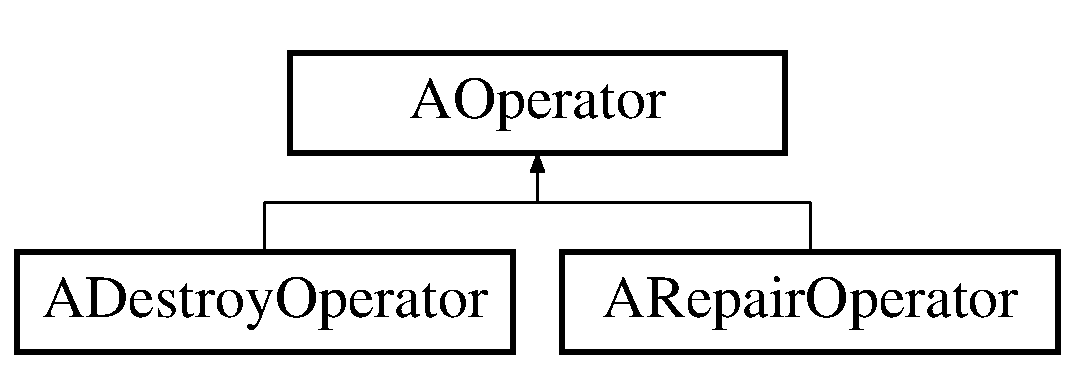
\includegraphics[height=2.000000cm]{classAOperator}
\end{center}
\end{figure}
\subsection*{\-Public \-Member \-Functions}
\begin{DoxyCompactItemize}
\item 
\hypertarget{classAOperator_afaaaafa72f7c09e64ecffd2ae83f6c29}{\hyperlink{classAOperator_afaaaafa72f7c09e64ecffd2ae83f6c29}{\-A\-Operator} (std\-::string name)}\label{classAOperator_afaaaafa72f7c09e64ecffd2ae83f6c29}

\begin{DoxyCompactList}\small\item\em \-Constructor. \end{DoxyCompactList}\item 
\hypertarget{classAOperator_a7854b2edbcad8022e3965076d5909f0e}{virtual \hyperlink{classAOperator_a7854b2edbcad8022e3965076d5909f0e}{$\sim$\-A\-Operator} ()}\label{classAOperator_a7854b2edbcad8022e3965076d5909f0e}

\begin{DoxyCompactList}\small\item\em \-Destructor. \end{DoxyCompactList}\item 
\hypertarget{classAOperator_aef1d7317fac50612783941a9ed4bdd55}{void \hyperlink{classAOperator_aef1d7317fac50612783941a9ed4bdd55}{init} ()}\label{classAOperator_aef1d7317fac50612783941a9ed4bdd55}

\begin{DoxyCompactList}\small\item\em \-Initialize the values of the numbers of calls. \end{DoxyCompactList}\item 
\hypertarget{classAOperator_a5e43e03617a73fc21764e8913cdbb023}{void \hyperlink{classAOperator_a5e43e03617a73fc21764e8913cdbb023}{reset\-Number\-Of\-Calls} ()}\label{classAOperator_a5e43e03617a73fc21764e8913cdbb023}

\begin{DoxyCompactList}\small\item\em reset the number of calls since last eval. \end{DoxyCompactList}\item 
size\-\_\-t \hyperlink{classAOperator_a53e8afe10d5ab0f717e0ee1771ac1e4e}{get\-Total\-Number\-Of\-Calls} ()
\item 
size\-\_\-t \hyperlink{classAOperator_aae3aa0fc70bbc10a61057d12856fd4a8}{get\-Number\-Of\-Calls\-Since\-Last\-Evaluation} ()
\item 
\hypertarget{classAOperator_a2d63ac666c67ec37a53e7098ecbbf2b2}{void {\bfseries increase\-Number\-Of\-Calls} ()}\label{classAOperator_a2d63ac666c67ec37a53e7098ecbbf2b2}

\item 
\hypertarget{classAOperator_ad5bf72a25f08aeef21b090543c057cd5}{double \hyperlink{classAOperator_ad5bf72a25f08aeef21b090543c057cd5}{get\-Score} () const }\label{classAOperator_ad5bf72a25f08aeef21b090543c057cd5}

\begin{DoxyCompactList}\small\item\em \-Simple getter. \end{DoxyCompactList}\item 
\hypertarget{classAOperator_a94bf714d3c808ea9d51a4665912d8761}{double \hyperlink{classAOperator_a94bf714d3c808ea9d51a4665912d8761}{get\-Weight} () const }\label{classAOperator_a94bf714d3c808ea9d51a4665912d8761}

\begin{DoxyCompactList}\small\item\em \-Simple getter. \end{DoxyCompactList}\item 
\hypertarget{classAOperator_a844c2d404aaedae38aac0f9260b520e3}{void \hyperlink{classAOperator_a844c2d404aaedae38aac0f9260b520e3}{reset\-Score} ()}\label{classAOperator_a844c2d404aaedae38aac0f9260b520e3}

\begin{DoxyCompactList}\small\item\em resetter. \end{DoxyCompactList}\item 
\hypertarget{classAOperator_ad49c57980dc06d58f2d5b586e073595c}{void \hyperlink{classAOperator_ad49c57980dc06d58f2d5b586e073595c}{set\-Score} (double s)}\label{classAOperator_ad49c57980dc06d58f2d5b586e073595c}

\begin{DoxyCompactList}\small\item\em \-Simple setter. \end{DoxyCompactList}\item 
\hypertarget{classAOperator_a89816ff814d27b6260d44f7cefa6112a}{void \hyperlink{classAOperator_a89816ff814d27b6260d44f7cefa6112a}{set\-Weight} (double weight)}\label{classAOperator_a89816ff814d27b6260d44f7cefa6112a}

\begin{DoxyCompactList}\small\item\em \-Simple setter. \end{DoxyCompactList}\item 
\hypertarget{classAOperator_a35536ffa9ce03396e5e453698d1a3591}{std\-::string \hyperlink{classAOperator_a35536ffa9ce03396e5e453698d1a3591}{get\-Name} ()}\label{classAOperator_a35536ffa9ce03396e5e453698d1a3591}

\begin{DoxyCompactList}\small\item\em \-Simple getter. \end{DoxyCompactList}\item 
\hypertarget{classAOperator_ae372929e08da0ad6fb960a4519f33a17}{void \hyperlink{classAOperator_ae372929e08da0ad6fb960a4519f33a17}{set\-Noise} ()}\label{classAOperator_ae372929e08da0ad6fb960a4519f33a17}

\begin{DoxyCompactList}\small\item\em \-Set noise to true. \end{DoxyCompactList}\item 
\hypertarget{classAOperator_ab1d6a25e233ec1383b9919f8dff098f1}{void \hyperlink{classAOperator_ab1d6a25e233ec1383b9919f8dff098f1}{unset\-Noise} ()}\label{classAOperator_ab1d6a25e233ec1383b9919f8dff098f1}

\begin{DoxyCompactList}\small\item\em \-Set noise to false. \end{DoxyCompactList}\end{DoxyCompactItemize}


\subsection{\-Detailed \-Description}
\-This abstract class represent an operator, \-Destroy and \-Repair \-Operators inherit from this class. 

\subsection{\-Member \-Function \-Documentation}
\hypertarget{classAOperator_aae3aa0fc70bbc10a61057d12856fd4a8}{\index{\-A\-Operator@{\-A\-Operator}!get\-Number\-Of\-Calls\-Since\-Last\-Evaluation@{get\-Number\-Of\-Calls\-Since\-Last\-Evaluation}}
\index{get\-Number\-Of\-Calls\-Since\-Last\-Evaluation@{get\-Number\-Of\-Calls\-Since\-Last\-Evaluation}!AOperator@{\-A\-Operator}}
\subsubsection[{get\-Number\-Of\-Calls\-Since\-Last\-Evaluation}]{\setlength{\rightskip}{0pt plus 5cm}size\-\_\-t {\bf \-A\-Operator\-::get\-Number\-Of\-Calls\-Since\-Last\-Evaluation} (
\begin{DoxyParamCaption}
{}
\end{DoxyParamCaption}
)\hspace{0.3cm}{\ttfamily  \mbox{[}inline\mbox{]}}}}\label{classAOperator_aae3aa0fc70bbc10a61057d12856fd4a8}
\-Simple getter. \begin{DoxyReturn}{\-Returns}
the number of calls to this operator since the last evaluation. 
\end{DoxyReturn}
\hypertarget{classAOperator_a53e8afe10d5ab0f717e0ee1771ac1e4e}{\index{\-A\-Operator@{\-A\-Operator}!get\-Total\-Number\-Of\-Calls@{get\-Total\-Number\-Of\-Calls}}
\index{get\-Total\-Number\-Of\-Calls@{get\-Total\-Number\-Of\-Calls}!AOperator@{\-A\-Operator}}
\subsubsection[{get\-Total\-Number\-Of\-Calls}]{\setlength{\rightskip}{0pt plus 5cm}size\-\_\-t {\bf \-A\-Operator\-::get\-Total\-Number\-Of\-Calls} (
\begin{DoxyParamCaption}
{}
\end{DoxyParamCaption}
)\hspace{0.3cm}{\ttfamily  \mbox{[}inline\mbox{]}}}}\label{classAOperator_a53e8afe10d5ab0f717e0ee1771ac1e4e}
\-Simple getter. \begin{DoxyReturn}{\-Returns}
the total number of calls to the operator since the beginning of the optimization process. 
\end{DoxyReturn}


\-The documentation for this class was generated from the following file\-:\begin{DoxyCompactItemize}
\item 
\-A\-L\-N\-S\-\_\-\-Static\-\_\-\-Lib/src/alns/\-A\-Operator.\-h\end{DoxyCompactItemize}

\hypertarget{classAOperatorManager}{\section{\-A\-Operator\-Manager \-Class \-Reference}
\label{classAOperatorManager}\index{\-A\-Operator\-Manager@{\-A\-Operator\-Manager}}
}
\-Inheritance diagram for \-A\-Operator\-Manager\-:\begin{figure}[H]
\begin{center}
\leavevmode
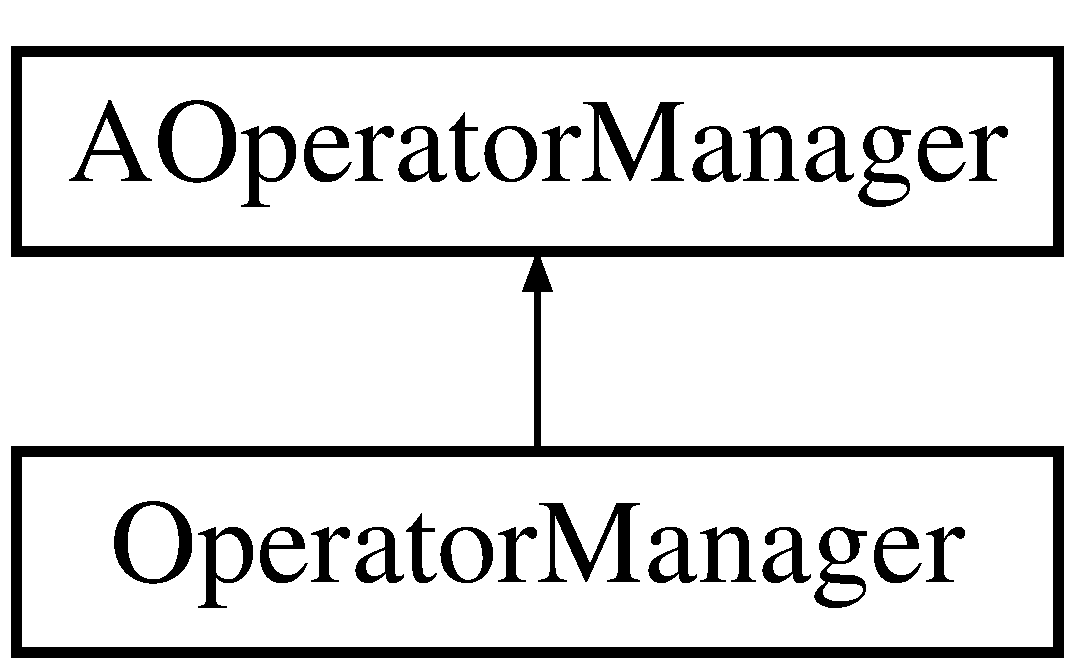
\includegraphics[height=2.000000cm]{classAOperatorManager}
\end{center}
\end{figure}
\subsection*{\-Public \-Member \-Functions}
\begin{DoxyCompactItemize}
\item 
virtual \hyperlink{classADestroyOperator}{\-A\-Destroy\-Operator} \& \hyperlink{classAOperatorManager_a0bafced8312c2d88e7006c08881750bc}{select\-Destroy\-Operator} ()=0
\item 
virtual \hyperlink{classARepairOperator}{\-A\-Repair\-Operator} \& \hyperlink{classAOperatorManager_a4258cef17ecd22b63804448dfd38ebcc}{select\-Repair\-Operator} ()=0
\item 
\hypertarget{classAOperatorManager_a83386737e04f631132490d4156e3c867}{virtual void {\bfseries recompute\-Weights} ()=0}\label{classAOperatorManager_a83386737e04f631132490d4156e3c867}

\item 
\hypertarget{classAOperatorManager_afb87eb820180a129287658c9a55487a0}{virtual void \hyperlink{classAOperatorManager_afb87eb820180a129287658c9a55487a0}{update\-Scores} (\hyperlink{classADestroyOperator}{\-A\-Destroy\-Operator} \&des, \hyperlink{classARepairOperator}{\-A\-Repair\-Operator} \&rep, \hyperlink{classALNS__Iteration__Status}{\-A\-L\-N\-S\-\_\-\-Iteration\-\_\-\-Status} \&status)=0}\label{classAOperatorManager_afb87eb820180a129287658c9a55487a0}

\begin{DoxyCompactList}\small\item\em \-Update the scores of the operators. \end{DoxyCompactList}\item 
\hypertarget{classAOperatorManager_afa1d2921a30cbd68c5fcaf1e76715a0f}{virtual void \hyperlink{classAOperatorManager_afa1d2921a30cbd68c5fcaf1e76715a0f}{start\-Signal} ()=0}\label{classAOperatorManager_afa1d2921a30cbd68c5fcaf1e76715a0f}

\begin{DoxyCompactList}\small\item\em \-Indicate that the optimization process starts. \end{DoxyCompactList}\item 
\hypertarget{classAOperatorManager_a838ee98f924be1924830e836889a00cb}{void \hyperlink{classAOperatorManager_a838ee98f924be1924830e836889a00cb}{set\-Statistics} (\hyperlink{classStatistics}{\-Statistics} $\ast$statistics)}\label{classAOperatorManager_a838ee98f924be1924830e836889a00cb}

\begin{DoxyCompactList}\small\item\em \-Simple setter. \end{DoxyCompactList}\end{DoxyCompactItemize}
\subsection*{\-Protected \-Attributes}
\begin{DoxyCompactItemize}
\item 
\hypertarget{classAOperatorManager_af08976002885d641241f160e0e419396}{\hyperlink{classStatistics}{\-Statistics} $\ast$ \hyperlink{classAOperatorManager_af08976002885d641241f160e0e419396}{stats}}\label{classAOperatorManager_af08976002885d641241f160e0e419396}

\begin{DoxyCompactList}\small\item\em \-A pointer to the instance of the statistics module. \end{DoxyCompactList}\end{DoxyCompactItemize}


\subsection{\-Member \-Function \-Documentation}
\hypertarget{classAOperatorManager_a0bafced8312c2d88e7006c08881750bc}{\index{\-A\-Operator\-Manager@{\-A\-Operator\-Manager}!select\-Destroy\-Operator@{select\-Destroy\-Operator}}
\index{select\-Destroy\-Operator@{select\-Destroy\-Operator}!AOperatorManager@{\-A\-Operator\-Manager}}
\subsubsection[{select\-Destroy\-Operator}]{\setlength{\rightskip}{0pt plus 5cm}virtual {\bf \-A\-Destroy\-Operator}\& {\bf \-A\-Operator\-Manager\-::select\-Destroy\-Operator} (
\begin{DoxyParamCaption}
{}
\end{DoxyParamCaption}
)\hspace{0.3cm}{\ttfamily  \mbox{[}pure virtual\mbox{]}}}}\label{classAOperatorManager_a0bafced8312c2d88e7006c08881750bc}
\-This method selects a destroy operator. \begin{DoxyReturn}{\-Returns}
a destroy operator. 
\end{DoxyReturn}


\-Implemented in \hyperlink{classOperatorManager_ae2b34fa76d49119d61836db181890085}{\-Operator\-Manager}.

\hypertarget{classAOperatorManager_a4258cef17ecd22b63804448dfd38ebcc}{\index{\-A\-Operator\-Manager@{\-A\-Operator\-Manager}!select\-Repair\-Operator@{select\-Repair\-Operator}}
\index{select\-Repair\-Operator@{select\-Repair\-Operator}!AOperatorManager@{\-A\-Operator\-Manager}}
\subsubsection[{select\-Repair\-Operator}]{\setlength{\rightskip}{0pt plus 5cm}virtual {\bf \-A\-Repair\-Operator}\& {\bf \-A\-Operator\-Manager\-::select\-Repair\-Operator} (
\begin{DoxyParamCaption}
{}
\end{DoxyParamCaption}
)\hspace{0.3cm}{\ttfamily  \mbox{[}pure virtual\mbox{]}}}}\label{classAOperatorManager_a4258cef17ecd22b63804448dfd38ebcc}
\-This method selects a repair operator. \begin{DoxyReturn}{\-Returns}
a repair operator. 
\end{DoxyReturn}


\-Implemented in \hyperlink{classOperatorManager_a620514b4b09095e5533e2fe3a44df529}{\-Operator\-Manager}.



\-The documentation for this class was generated from the following file\-:\begin{DoxyCompactItemize}
\item 
\-A\-L\-N\-S\-\_\-\-Static\-\_\-\-Lib/src/alns/\-A\-Operator\-Manager.\-h\end{DoxyCompactItemize}

\hypertarget{classARepairOperator}{\section{\-A\-Repair\-Operator \-Class \-Reference}
\label{classARepairOperator}\index{\-A\-Repair\-Operator@{\-A\-Repair\-Operator}}
}


\-This abstract class represent a \-Repair \-Operator, all repair operator implementations should inherit from this class.  




{\ttfamily \#include $<$\-A\-Repair\-Operator.\-h$>$}

\-Inheritance diagram for \-A\-Repair\-Operator\-:\begin{figure}[H]
\begin{center}
\leavevmode
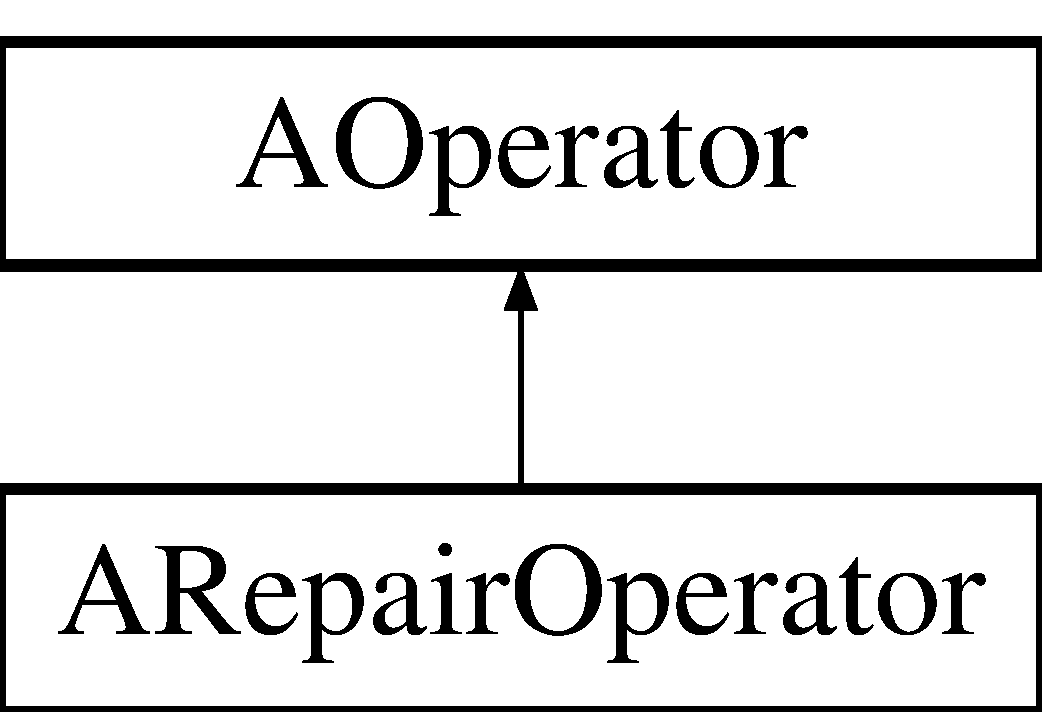
\includegraphics[height=2.000000cm]{classARepairOperator}
\end{center}
\end{figure}
\subsection*{\-Public \-Member \-Functions}
\begin{DoxyCompactItemize}
\item 
\hypertarget{classARepairOperator_a89708148ed12ce96048911c8b1c54a4c}{{\bfseries \-A\-Repair\-Operator} (std\-::string s)}\label{classARepairOperator_a89708148ed12ce96048911c8b1c54a4c}

\item 
\hypertarget{classARepairOperator_a0192890e73c77197ae8591991169cdca}{virtual void {\bfseries repair\-Solution} (\hyperlink{classISolution}{\-I\-Solution} \&sol)=0}\label{classARepairOperator_a0192890e73c77197ae8591991169cdca}

\end{DoxyCompactItemize}


\subsection{\-Detailed \-Description}
\-This abstract class represent a \-Repair \-Operator, all repair operator implementations should inherit from this class. 

\-The documentation for this class was generated from the following file\-:\begin{DoxyCompactItemize}
\item 
\-A\-L\-N\-S\-\_\-\-Static\-\_\-\-Lib/src/alns/\-A\-Repair\-Operator.\-h\end{DoxyCompactItemize}

\hypertarget{classCoolingSchedule__Parameters}{\section{\-Cooling\-Schedule\-\_\-\-Parameters \-Class \-Reference}
\label{classCoolingSchedule__Parameters}\index{\-Cooling\-Schedule\-\_\-\-Parameters@{\-Cooling\-Schedule\-\_\-\-Parameters}}
}


\-This class represent parameters to be used to instantiate cooling schedules.  




{\ttfamily \#include $<$\-Cooling\-Schedule\-\_\-\-Parameters.\-h$>$}

\subsection*{\-Public \-Types}
\begin{DoxyCompactItemize}
\item 
enum \hyperlink{classCoolingSchedule__Parameters_a8f5c0d2aabf39957308a738d88c2f16a}{\-C\-S\-Kind} \{ \*
{\bfseries \-Linear\-\_\-it}, 
{\bfseries \-Linear\-\_\-time}, 
{\bfseries \-Linear\-\_\-mix}, 
{\bfseries \-Exponential\-\_\-it}, 
\*
{\bfseries \-Exponential\-\_\-time}, 
{\bfseries \-Exponential\-\_\-mix}
 \}
\begin{DoxyCompactList}\small\item\em \-Enumeration representing the various kind of cooling schedules that can be handled. \end{DoxyCompactList}\end{DoxyCompactItemize}
\subsection*{\-Public \-Member \-Functions}
\begin{DoxyCompactItemize}
\item 
\hypertarget{classCoolingSchedule__Parameters_aa55a639451c12ef5c97eb0fab6314947}{\hyperlink{classCoolingSchedule__Parameters_aa55a639451c12ef5c97eb0fab6314947}{\-Cooling\-Schedule\-\_\-\-Parameters} (\hyperlink{classALNS__Parameters}{\-A\-L\-N\-S\-\_\-\-Parameters} \&alns\-Param)}\label{classCoolingSchedule__Parameters_aa55a639451c12ef5c97eb0fab6314947}

\begin{DoxyCompactList}\small\item\em \-Constructor. \end{DoxyCompactList}\item 
\hypertarget{classCoolingSchedule__Parameters_af5a521c2ccc81e1d2406ebf99b644881}{\hyperlink{classCoolingSchedule__Parameters_af5a521c2ccc81e1d2406ebf99b644881}{$\sim$\-Cooling\-Schedule\-\_\-\-Parameters} ()}\label{classCoolingSchedule__Parameters_af5a521c2ccc81e1d2406ebf99b644881}

\begin{DoxyCompactList}\small\item\em \-Destructor. \end{DoxyCompactList}\item 
\hypertarget{classCoolingSchedule__Parameters_aa0241491f174761ed09d7f451351c3c3}{void \hyperlink{classCoolingSchedule__Parameters_aa0241491f174761ed09d7f451351c3c3}{sanity\-Checks} ()}\label{classCoolingSchedule__Parameters_aa0241491f174761ed09d7f451351c3c3}

\begin{DoxyCompactList}\small\item\em \-Perform some sanity checks on the values of the parameters. \end{DoxyCompactList}\item 
void \hyperlink{classCoolingSchedule__Parameters_a3d668de3af41138374b459c023e53b55}{load\-Parameters} (std\-::string path)
\end{DoxyCompactItemize}
\subsection*{\-Public \-Attributes}
\begin{DoxyCompactItemize}
\item 
\hypertarget{classCoolingSchedule__Parameters_ad7c13cb862526a5f104105a7139c1a79}{\hyperlink{classCoolingSchedule__Parameters_a8f5c0d2aabf39957308a738d88c2f16a}{\-C\-S\-Kind} \hyperlink{classCoolingSchedule__Parameters_ad7c13cb862526a5f104105a7139c1a79}{kind}}\label{classCoolingSchedule__Parameters_ad7c13cb862526a5f104105a7139c1a79}

\begin{DoxyCompactList}\small\item\em \-The kind of cooling schedule to be used. \end{DoxyCompactList}\item 
double \hyperlink{classCoolingSchedule__Parameters_a288ef5bba5e1b04f1e00c83a8664f7b8}{exp\-Percentage\-Kept}
\item 
double \hyperlink{classCoolingSchedule__Parameters_a11baeae90fe80f917c33703e8b456f32}{setup\-Percentage}
\item 
\hypertarget{classCoolingSchedule__Parameters_a0975632fdd8eef8bbdb843d3898e6813}{size\-\_\-t \hyperlink{classCoolingSchedule__Parameters_a0975632fdd8eef8bbdb843d3898e6813}{nb\-Thresholds}}\label{classCoolingSchedule__Parameters_a0975632fdd8eef8bbdb843d3898e6813}

\begin{DoxyCompactList}\small\item\em \-The number of temperature recomputations during the optimization process. \end{DoxyCompactList}\item 
\hypertarget{classCoolingSchedule__Parameters_a91947e9b5d48723480502a295d1114fd}{size\-\_\-t \hyperlink{classCoolingSchedule__Parameters_a91947e9b5d48723480502a295d1114fd}{max\-It}}\label{classCoolingSchedule__Parameters_a91947e9b5d48723480502a295d1114fd}

\begin{DoxyCompactList}\small\item\em \-The maximum number of iterations. \end{DoxyCompactList}\item 
\hypertarget{classCoolingSchedule__Parameters_aa14ff24f11c1a4e9b365889cf2223442}{size\-\_\-t \hyperlink{classCoolingSchedule__Parameters_aa14ff24f11c1a4e9b365889cf2223442}{max\-R\-T}}\label{classCoolingSchedule__Parameters_aa14ff24f11c1a4e9b365889cf2223442}

\begin{DoxyCompactList}\small\item\em \-The maximum running time. \end{DoxyCompactList}\end{DoxyCompactItemize}


\subsection{\-Detailed \-Description}
\-This class represent parameters to be used to instantiate cooling schedules. 

\subsection{\-Member \-Function \-Documentation}
\hypertarget{classCoolingSchedule__Parameters_a3d668de3af41138374b459c023e53b55}{\index{\-Cooling\-Schedule\-\_\-\-Parameters@{\-Cooling\-Schedule\-\_\-\-Parameters}!load\-Parameters@{load\-Parameters}}
\index{load\-Parameters@{load\-Parameters}!CoolingSchedule_Parameters@{\-Cooling\-Schedule\-\_\-\-Parameters}}
\subsubsection[{load\-Parameters}]{\setlength{\rightskip}{0pt plus 5cm}void {\bf \-Cooling\-Schedule\-\_\-\-Parameters\-::load\-Parameters} (
\begin{DoxyParamCaption}
\item[{std\-::string}]{path}
\end{DoxyParamCaption}
)}}\label{classCoolingSchedule__Parameters_a3d668de3af41138374b459c023e53b55}
\-Load the parameters from a text file. 
\begin{DoxyParams}{\-Parameters}
{\em path} & the path to the text file containing the parameters. \\
\hline
\end{DoxyParams}


\subsection{\-Member \-Data \-Documentation}
\hypertarget{classCoolingSchedule__Parameters_a288ef5bba5e1b04f1e00c83a8664f7b8}{\index{\-Cooling\-Schedule\-\_\-\-Parameters@{\-Cooling\-Schedule\-\_\-\-Parameters}!exp\-Percentage\-Kept@{exp\-Percentage\-Kept}}
\index{exp\-Percentage\-Kept@{exp\-Percentage\-Kept}!CoolingSchedule_Parameters@{\-Cooling\-Schedule\-\_\-\-Parameters}}
\subsubsection[{exp\-Percentage\-Kept}]{\setlength{\rightskip}{0pt plus 5cm}double {\bf \-Cooling\-Schedule\-\_\-\-Parameters\-::exp\-Percentage\-Kept}}}\label{classCoolingSchedule__Parameters_a288ef5bba5e1b04f1e00c83a8664f7b8}
\-In case of the use of an exponential cooling schedule, the percentage of the current temperature kept at each temperature recomputation. \hypertarget{classCoolingSchedule__Parameters_a11baeae90fe80f917c33703e8b456f32}{\index{\-Cooling\-Schedule\-\_\-\-Parameters@{\-Cooling\-Schedule\-\_\-\-Parameters}!setup\-Percentage@{setup\-Percentage}}
\index{setup\-Percentage@{setup\-Percentage}!CoolingSchedule_Parameters@{\-Cooling\-Schedule\-\_\-\-Parameters}}
\subsubsection[{setup\-Percentage}]{\setlength{\rightskip}{0pt plus 5cm}double {\bf \-Cooling\-Schedule\-\_\-\-Parameters\-::setup\-Percentage}}}\label{classCoolingSchedule__Parameters_a11baeae90fe80f917c33703e8b456f32}
\-To determine the starting temperature, how worse than the initial solution can a solution be to have a 50\% chance of being accepted at the starting temperature. 

\-The documentation for this class was generated from the following files\-:\begin{DoxyCompactItemize}
\item 
\-A\-L\-N\-S\-\_\-\-Static\-\_\-\-Lib/src/acceptance\-Module/\-Cooling\-Schedule\-\_\-\-Parameters.\-h\item 
\-A\-L\-N\-S\-\_\-\-Static\-\_\-\-Lib/src/acceptance\-Module/\-Cooling\-Schedule\-\_\-\-Parameters.\-cpp\end{DoxyCompactItemize}

\hypertarget{classCoolingScheduleFactory}{\section{\-Cooling\-Schedule\-Factory \-Class \-Reference}
\label{classCoolingScheduleFactory}\index{\-Cooling\-Schedule\-Factory@{\-Cooling\-Schedule\-Factory}}
}


\-This class instantiate cooling schedules.  




{\ttfamily \#include $<$\-Cooling\-Schedule\-Factory.\-h$>$}

\subsection*{\-Static \-Public \-Member \-Functions}
\begin{DoxyCompactItemize}
\item 
static \hyperlink{classICoolingSchedule}{\-I\-Cooling\-Schedule} $\ast$ \hyperlink{classCoolingScheduleFactory_a6ece4797b00faef894e6160e050ddfc0}{make\-Cooling\-Schedule} (\hyperlink{classISolution}{\-I\-Solution} \&sol, \hyperlink{classCoolingSchedule__Parameters}{\-Cooling\-Schedule\-\_\-\-Parameters} \&param)
\end{DoxyCompactItemize}


\subsection{\-Detailed \-Description}
\-This class instantiate cooling schedules. 

\subsection{\-Member \-Function \-Documentation}
\hypertarget{classCoolingScheduleFactory_a6ece4797b00faef894e6160e050ddfc0}{\index{\-Cooling\-Schedule\-Factory@{\-Cooling\-Schedule\-Factory}!make\-Cooling\-Schedule@{make\-Cooling\-Schedule}}
\index{make\-Cooling\-Schedule@{make\-Cooling\-Schedule}!CoolingScheduleFactory@{\-Cooling\-Schedule\-Factory}}
\subsubsection[{make\-Cooling\-Schedule}]{\setlength{\rightskip}{0pt plus 5cm}{\bf \-I\-Cooling\-Schedule} $\ast$ {\bf \-Cooling\-Schedule\-Factory\-::make\-Cooling\-Schedule} (
\begin{DoxyParamCaption}
\item[{{\bf \-I\-Solution} \&}]{sol, }
\item[{{\bf \-Cooling\-Schedule\-\_\-\-Parameters} \&}]{param}
\end{DoxyParamCaption}
)\hspace{0.3cm}{\ttfamily  \mbox{[}static\mbox{]}}}}\label{classCoolingScheduleFactory_a6ece4797b00faef894e6160e050ddfc0}
\-Generate a cooling schedule using the initial solution and the cooling schedule parameters. 
\begin{DoxyParams}{\-Parameters}
{\em sol} & the initial solution. \\
\hline
{\em param} & the parameters to be used to generate the cooling schedule. \\
\hline
\end{DoxyParams}
\begin{DoxyReturn}{\-Returns}
a pointer to a cooling schedule. 
\end{DoxyReturn}


\-The documentation for this class was generated from the following files\-:\begin{DoxyCompactItemize}
\item 
\-A\-L\-N\-S\-\_\-\-Static\-\_\-\-Lib/src/acceptance\-Module/\-Cooling\-Schedule\-Factory.\-h\item 
\-A\-L\-N\-S\-\_\-\-Static\-\_\-\-Lib/src/acceptance\-Module/\-Cooling\-Schedule\-Factory.\-cpp\end{DoxyCompactItemize}

\hypertarget{classDummyAcceptanceModule}{\section{\-Dummy\-Acceptance\-Module \-Class \-Reference}
\label{classDummyAcceptanceModule}\index{\-Dummy\-Acceptance\-Module@{\-Dummy\-Acceptance\-Module}}
}


\-This module accept any solution as the current solution.  




{\ttfamily \#include $<$\-Dummy\-Acceptance\-Module.\-h$>$}

\-Inheritance diagram for \-Dummy\-Acceptance\-Module\-:\begin{figure}[H]
\begin{center}
\leavevmode
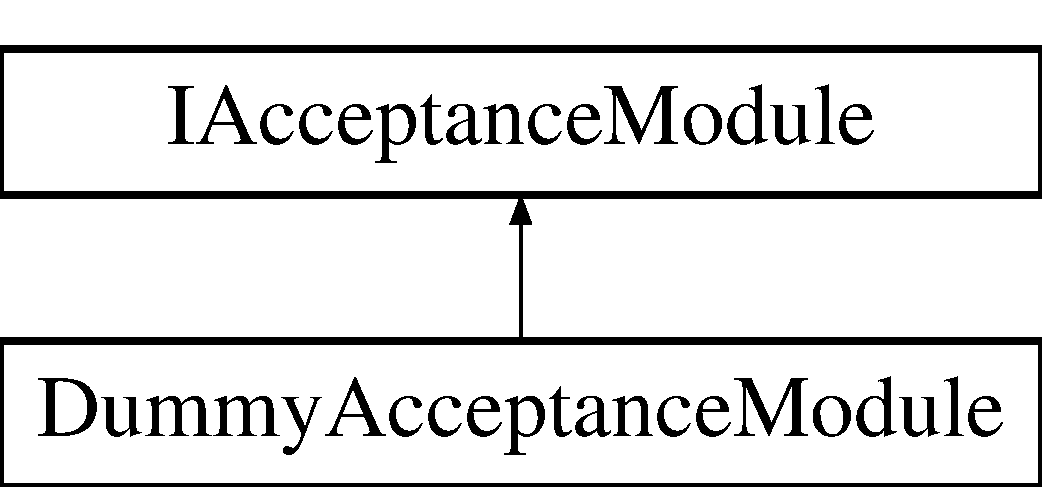
\includegraphics[height=2.000000cm]{classDummyAcceptanceModule}
\end{center}
\end{figure}
\subsection*{\-Public \-Member \-Functions}
\begin{DoxyCompactItemize}
\item 
\hypertarget{classDummyAcceptanceModule_ab906bf78a974bbe427ed861b74d7ae79}{\hyperlink{classDummyAcceptanceModule_ab906bf78a974bbe427ed861b74d7ae79}{\-Dummy\-Acceptance\-Module} ()}\label{classDummyAcceptanceModule_ab906bf78a974bbe427ed861b74d7ae79}

\begin{DoxyCompactList}\small\item\em \-Constructor. \end{DoxyCompactList}\item 
\hypertarget{classDummyAcceptanceModule_a7e2568aa7b42a6e06d7b3d962a1ff721}{virtual \hyperlink{classDummyAcceptanceModule_a7e2568aa7b42a6e06d7b3d962a1ff721}{$\sim$\-Dummy\-Acceptance\-Module} ()}\label{classDummyAcceptanceModule_a7e2568aa7b42a6e06d7b3d962a1ff721}

\begin{DoxyCompactList}\small\item\em \-Destructor. \end{DoxyCompactList}\item 
\hypertarget{classDummyAcceptanceModule_a0db83ebfd5f38764dcd7a747cf3feb5a}{bool \hyperlink{classDummyAcceptanceModule_a0db83ebfd5f38764dcd7a747cf3feb5a}{transition\-Accepted} (\hyperlink{classIBestSolutionManager}{\-I\-Best\-Solution\-Manager} \&best\-Solution\-Manager, \hyperlink{classISolution}{\-I\-Solution} \&current\-Solution, \hyperlink{classISolution}{\-I\-Solution} \&new\-Solution, \hyperlink{classALNS__Iteration__Status}{\-A\-L\-N\-S\-\_\-\-Iteration\-\_\-\-Status} \&status)}\label{classDummyAcceptanceModule_a0db83ebfd5f38764dcd7a747cf3feb5a}

\begin{DoxyCompactList}\small\item\em \-Compute if the newly created solution have to be accepted or not. \end{DoxyCompactList}\end{DoxyCompactItemize}


\subsection{\-Detailed \-Description}
\-This module accept any solution as the current solution. 

\-It can be used when the diversification is ensured through an other mechanism. \-For example when the operators embbed some tabu criterion to prevent them from rebuilding the previous solution. 

\-The documentation for this class was generated from the following files\-:\begin{DoxyCompactItemize}
\item 
\-A\-L\-N\-S\-\_\-\-Static\-\_\-\-Lib/src/acceptance\-Module/\-Dummy\-Acceptance\-Module.\-h\item 
\-A\-L\-N\-S\-\_\-\-Static\-\_\-\-Lib/src/acceptance\-Module/\-Dummy\-Acceptance\-Module.\-cpp\end{DoxyCompactItemize}

\hypertarget{classExponentialCoolingSchedule}{\section{\-Exponential\-Cooling\-Schedule \-Class \-Reference}
\label{classExponentialCoolingSchedule}\index{\-Exponential\-Cooling\-Schedule@{\-Exponential\-Cooling\-Schedule}}
}


\-An exponential cooling schedule based on a mix of the maximum running time and the number of iterations.  




{\ttfamily \#include $<$\-Exponential\-Cooling\-Schedule.\-h$>$}

\-Inheritance diagram for \-Exponential\-Cooling\-Schedule\-:\begin{figure}[H]
\begin{center}
\leavevmode
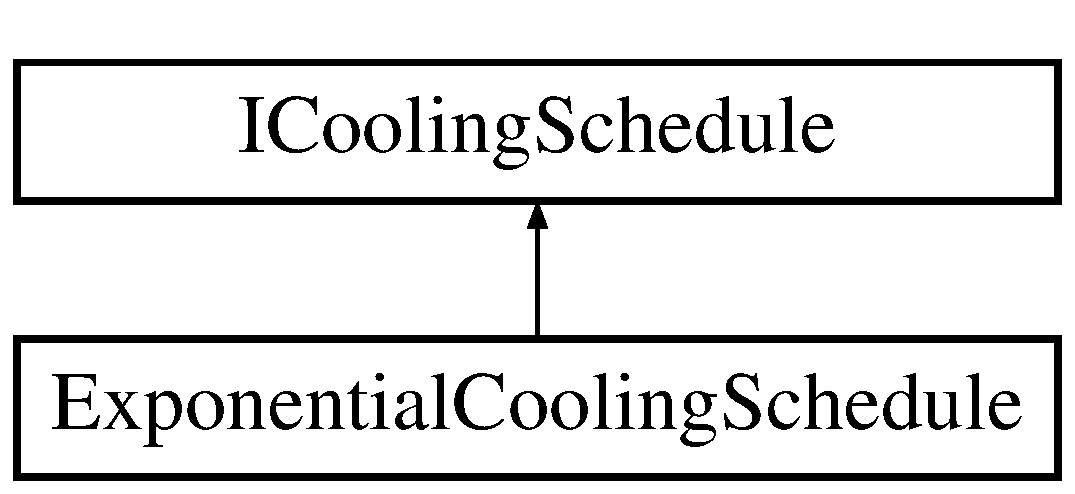
\includegraphics[height=2.000000cm]{classExponentialCoolingSchedule}
\end{center}
\end{figure}
\subsection*{\-Public \-Member \-Functions}
\begin{DoxyCompactItemize}
\item 
\hyperlink{classExponentialCoolingSchedule_a41341124cd5cac5e92bf90d78d967462}{\-Exponential\-Cooling\-Schedule} (\hyperlink{classISolution}{\-I\-Solution} \&init\-Sol, \hyperlink{classCoolingSchedule__Parameters}{\-Cooling\-Schedule\-\_\-\-Parameters} \&cs\-Param)
\item 
\hypertarget{classExponentialCoolingSchedule_a28ec19b3dd2a2da22132027de5119d5f}{virtual \hyperlink{classExponentialCoolingSchedule_a28ec19b3dd2a2da22132027de5119d5f}{$\sim$\-Exponential\-Cooling\-Schedule} ()}\label{classExponentialCoolingSchedule_a28ec19b3dd2a2da22132027de5119d5f}

\begin{DoxyCompactList}\small\item\em \-Destructor. \end{DoxyCompactList}\item 
double \hyperlink{classExponentialCoolingSchedule_ac32efff552a53ff64ff00deb490b1cb7}{get\-Current\-Temperature} ()
\item 
\hypertarget{classExponentialCoolingSchedule_a64b6a3c4b329b18ca55c68d75cb03a00}{virtual void \hyperlink{classExponentialCoolingSchedule_a64b6a3c4b329b18ca55c68d75cb03a00}{start\-Signal} ()}\label{classExponentialCoolingSchedule_a64b6a3c4b329b18ca55c68d75cb03a00}

\begin{DoxyCompactList}\small\item\em \-This method is called when the optimization process start. \end{DoxyCompactList}\end{DoxyCompactItemize}


\subsection{\-Detailed \-Description}
\-An exponential cooling schedule based on a mix of the maximum running time and the number of iterations. 

\subsection{\-Constructor \& \-Destructor \-Documentation}
\hypertarget{classExponentialCoolingSchedule_a41341124cd5cac5e92bf90d78d967462}{\index{\-Exponential\-Cooling\-Schedule@{\-Exponential\-Cooling\-Schedule}!\-Exponential\-Cooling\-Schedule@{\-Exponential\-Cooling\-Schedule}}
\index{\-Exponential\-Cooling\-Schedule@{\-Exponential\-Cooling\-Schedule}!ExponentialCoolingSchedule@{\-Exponential\-Cooling\-Schedule}}
\subsubsection[{\-Exponential\-Cooling\-Schedule}]{\setlength{\rightskip}{0pt plus 5cm}{\bf \-Exponential\-Cooling\-Schedule\-::\-Exponential\-Cooling\-Schedule} (
\begin{DoxyParamCaption}
\item[{{\bf \-I\-Solution} \&}]{init\-Sol, }
\item[{{\bf \-Cooling\-Schedule\-\_\-\-Parameters} \&}]{cs\-Param}
\end{DoxyParamCaption}
)}}\label{classExponentialCoolingSchedule_a41341124cd5cac5e92bf90d78d967462}
\-Constructor. 
\begin{DoxyParams}{\-Parameters}
{\em init\-Sol} & the initial solution. \\
\hline
{\em cs\-Param} & the cooling schedule parameters to be used. \\
\hline
\end{DoxyParams}


\subsection{\-Member \-Function \-Documentation}
\hypertarget{classExponentialCoolingSchedule_ac32efff552a53ff64ff00deb490b1cb7}{\index{\-Exponential\-Cooling\-Schedule@{\-Exponential\-Cooling\-Schedule}!get\-Current\-Temperature@{get\-Current\-Temperature}}
\index{get\-Current\-Temperature@{get\-Current\-Temperature}!ExponentialCoolingSchedule@{\-Exponential\-Cooling\-Schedule}}
\subsubsection[{get\-Current\-Temperature}]{\setlength{\rightskip}{0pt plus 5cm}double {\bf \-Exponential\-Cooling\-Schedule\-::get\-Current\-Temperature} (
\begin{DoxyParamCaption}
{}
\end{DoxyParamCaption}
)\hspace{0.3cm}{\ttfamily  \mbox{[}virtual\mbox{]}}}}\label{classExponentialCoolingSchedule_ac32efff552a53ff64ff00deb490b1cb7}
\-Compute and return the current temperature. \begin{DoxyReturn}{\-Returns}
the current temperature. 
\end{DoxyReturn}


\-Implements \hyperlink{classICoolingSchedule_ac5d2dbf784cde3a36fd5e7c5c3fbdd96}{\-I\-Cooling\-Schedule}.



\-The documentation for this class was generated from the following files\-:\begin{DoxyCompactItemize}
\item 
\-A\-L\-N\-S\-\_\-\-Static\-\_\-\-Lib/src/acceptance\-Module/\-Exponential\-Cooling\-Schedule.\-h\item 
\-A\-L\-N\-S\-\_\-\-Static\-\_\-\-Lib/src/acceptance\-Module/\-Exponential\-Cooling\-Schedule.\-cpp\end{DoxyCompactItemize}

\hypertarget{classIAcceptanceModule}{\section{\-I\-Acceptance\-Module \-Class \-Reference}
\label{classIAcceptanceModule}\index{\-I\-Acceptance\-Module@{\-I\-Acceptance\-Module}}
}


\-This is an interface to define acceptance modules within the \hyperlink{classALNS}{\-A\-L\-N\-S}.  




{\ttfamily \#include $<$\-I\-Acceptance\-Module.\-h$>$}

\-Inheritance diagram for \-I\-Acceptance\-Module\-:\begin{figure}[H]
\begin{center}
\leavevmode
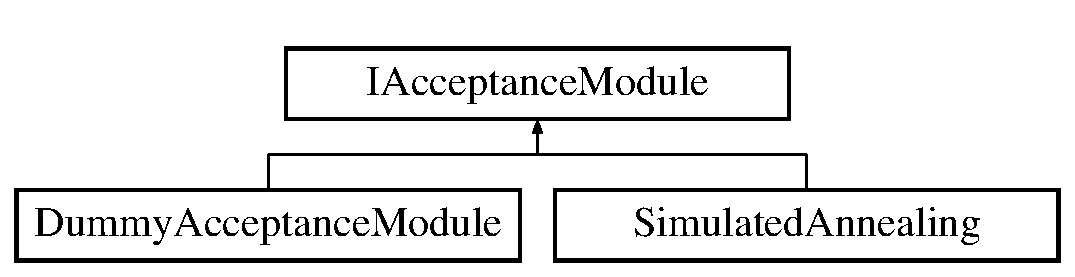
\includegraphics[height=2.000000cm]{classIAcceptanceModule}
\end{center}
\end{figure}
\subsection*{\-Public \-Member \-Functions}
\begin{DoxyCompactItemize}
\item 
virtual bool \hyperlink{classIAcceptanceModule_a47655425cbbbd5ff70106214169a7f1c}{transition\-Accepted} (\hyperlink{classIBestSolutionManager}{\-I\-Best\-Solution\-Manager} \&best\-Solution\-Manager, \hyperlink{classISolution}{\-I\-Solution} \&current\-Solution, \hyperlink{classISolution}{\-I\-Solution} \&new\-Solution, \hyperlink{classALNS__Iteration__Status}{\-A\-L\-N\-S\-\_\-\-Iteration\-\_\-\-Status} \&status)=0
\item 
virtual void \hyperlink{classIAcceptanceModule_adf6b1054982d528815e339aa8a829d4a}{start\-Signal} ()
\end{DoxyCompactItemize}


\subsection{\-Detailed \-Description}
\-This is an interface to define acceptance modules within the \hyperlink{classALNS}{\-A\-L\-N\-S}. 

\subsection{\-Member \-Function \-Documentation}
\hypertarget{classIAcceptanceModule_adf6b1054982d528815e339aa8a829d4a}{\index{\-I\-Acceptance\-Module@{\-I\-Acceptance\-Module}!start\-Signal@{start\-Signal}}
\index{start\-Signal@{start\-Signal}!IAcceptanceModule@{\-I\-Acceptance\-Module}}
\subsubsection[{start\-Signal}]{\setlength{\rightskip}{0pt plus 5cm}virtual void {\bf \-I\-Acceptance\-Module\-::start\-Signal} (
\begin{DoxyParamCaption}
{}
\end{DoxyParamCaption}
)\hspace{0.3cm}{\ttfamily  \mbox{[}inline, virtual\mbox{]}}}}\label{classIAcceptanceModule_adf6b1054982d528815e339aa8a829d4a}
\-Some \-Acceptance modules needs to initialize some variable only when the solver actualy starts working. \-In this case you should override this method. 

\-Reimplemented in \hyperlink{classSimulatedAnnealing_a13ddd574a0528f64801016a235ec8ee3}{\-Simulated\-Annealing}.

\hypertarget{classIAcceptanceModule_a47655425cbbbd5ff70106214169a7f1c}{\index{\-I\-Acceptance\-Module@{\-I\-Acceptance\-Module}!transition\-Accepted@{transition\-Accepted}}
\index{transition\-Accepted@{transition\-Accepted}!IAcceptanceModule@{\-I\-Acceptance\-Module}}
\subsubsection[{transition\-Accepted}]{\setlength{\rightskip}{0pt plus 5cm}virtual bool {\bf \-I\-Acceptance\-Module\-::transition\-Accepted} (
\begin{DoxyParamCaption}
\item[{{\bf \-I\-Best\-Solution\-Manager} \&}]{best\-Solution\-Manager, }
\item[{{\bf \-I\-Solution} \&}]{current\-Solution, }
\item[{{\bf \-I\-Solution} \&}]{new\-Solution, }
\item[{{\bf \-A\-L\-N\-S\-\_\-\-Iteration\-\_\-\-Status} \&}]{status}
\end{DoxyParamCaption}
)\hspace{0.3cm}{\ttfamily  \mbox{[}pure virtual\mbox{]}}}}\label{classIAcceptanceModule_a47655425cbbbd5ff70106214169a7f1c}
\-Indicate if the new created solution have to be accepted or not 
\begin{DoxyParams}{\-Parameters}
{\em best\-Solution\-Manager} & a reference to the best solution manager. \\
\hline
{\em current\-Solution} & current solution. \\
\hline
{\em new\-Solution} & new solution. \\
\hline
{\em status} & the status of the current alns iteration. \\
\hline
\end{DoxyParams}
\begin{DoxyReturn}{\-Returns}
true if the transition is accepted, false otherwise. 
\end{DoxyReturn}


\-Implemented in \hyperlink{classSimulatedAnnealing_a1bea2151b5c2b9b18f16bb47337af3cc}{\-Simulated\-Annealing}, and \hyperlink{classDummyAcceptanceModule_a0db83ebfd5f38764dcd7a747cf3feb5a}{\-Dummy\-Acceptance\-Module}.



\-The documentation for this class was generated from the following file\-:\begin{DoxyCompactItemize}
\item 
\-A\-L\-N\-S\-\_\-\-Static\-\_\-\-Lib/src/acceptance\-Module/\-I\-Acceptance\-Module.\-h\end{DoxyCompactItemize}

\hypertarget{classIBestSolutionManager}{\section{\-I\-Best\-Solution\-Manager \-Class \-Reference}
\label{classIBestSolutionManager}\index{\-I\-Best\-Solution\-Manager@{\-I\-Best\-Solution\-Manager}}
}
\-Inheritance diagram for \-I\-Best\-Solution\-Manager\-:\begin{figure}[H]
\begin{center}
\leavevmode
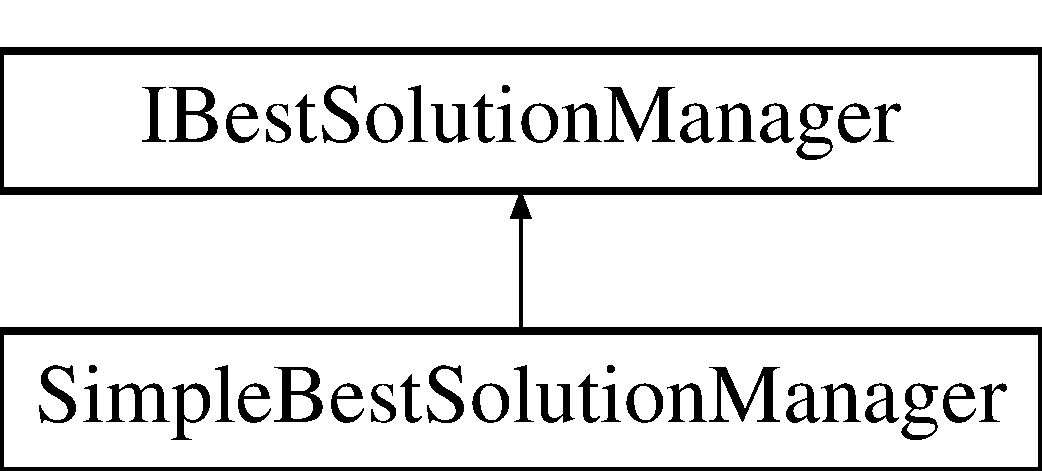
\includegraphics[height=2.000000cm]{classIBestSolutionManager}
\end{center}
\end{figure}
\subsection*{\-Public \-Member \-Functions}
\begin{DoxyCompactItemize}
\item 
virtual bool \hyperlink{classIBestSolutionManager_adf056afba7bfda2b3a3260d8118d5c44}{is\-New\-Best\-Solution} (\hyperlink{classISolution}{\-I\-Solution} \&sol)=0
\item 
\hypertarget{classIBestSolutionManager_ab4f9c16464364b2a3b9b45a0453a32d1}{virtual std\-::list$<$ \hyperlink{classISolution}{\-I\-Solution} $\ast$ $>$\*
\-::iterator \hyperlink{classIBestSolutionManager_ab4f9c16464364b2a3b9b45a0453a32d1}{begin} ()=0}\label{classIBestSolutionManager_ab4f9c16464364b2a3b9b45a0453a32d1}

\begin{DoxyCompactList}\small\item\em \-Return a pointer to a best solution. \end{DoxyCompactList}\item 
\hypertarget{classIBestSolutionManager_ade090d69dfaa3bb36f2b5b21bf652c8f}{virtual std\-::list$<$ \hyperlink{classISolution}{\-I\-Solution} $\ast$ $>$\*
\-::iterator \hyperlink{classIBestSolutionManager_ade090d69dfaa3bb36f2b5b21bf652c8f}{end} ()=0}\label{classIBestSolutionManager_ade090d69dfaa3bb36f2b5b21bf652c8f}

\begin{DoxyCompactList}\small\item\em \-Return a pointer to a best solution. \end{DoxyCompactList}\item 
virtual \hyperlink{classISolution}{\-I\-Solution} $\ast$ \hyperlink{classIBestSolutionManager_a592e8c6de9b295e834ef04f52ae376a6}{reload\-Best\-Solution} (\hyperlink{classISolution}{\-I\-Solution} $\ast$curr\-Sol, \hyperlink{classALNS__Iteration__Status}{\-A\-L\-N\-S\-\_\-\-Iteration\-\_\-\-Status} \&status)=0
\end{DoxyCompactItemize}


\subsection{\-Member \-Function \-Documentation}
\hypertarget{classIBestSolutionManager_adf056afba7bfda2b3a3260d8118d5c44}{\index{\-I\-Best\-Solution\-Manager@{\-I\-Best\-Solution\-Manager}!is\-New\-Best\-Solution@{is\-New\-Best\-Solution}}
\index{is\-New\-Best\-Solution@{is\-New\-Best\-Solution}!IBestSolutionManager@{\-I\-Best\-Solution\-Manager}}
\subsubsection[{is\-New\-Best\-Solution}]{\setlength{\rightskip}{0pt plus 5cm}virtual bool {\bf \-I\-Best\-Solution\-Manager\-::is\-New\-Best\-Solution} (
\begin{DoxyParamCaption}
\item[{{\bf \-I\-Solution} \&}]{sol}
\end{DoxyParamCaption}
)\hspace{0.3cm}{\ttfamily  \mbox{[}pure virtual\mbox{]}}}}\label{classIBestSolutionManager_adf056afba7bfda2b3a3260d8118d5c44}
\-This method evaluate if a solution is a new best solution, and adds it to the best solution pool in this case. 
\begin{DoxyParams}{\-Parameters}
{\em sol} & the solution to be tested. \\
\hline
\end{DoxyParams}
\begin{DoxyReturn}{\-Returns}
true if the solution is a new best solution, false otherwise. 
\end{DoxyReturn}


\-Implemented in \hyperlink{classSimpleBestSolutionManager_a8237e1d633717d3dc69c35ff5a88497a}{\-Simple\-Best\-Solution\-Manager}.

\hypertarget{classIBestSolutionManager_a592e8c6de9b295e834ef04f52ae376a6}{\index{\-I\-Best\-Solution\-Manager@{\-I\-Best\-Solution\-Manager}!reload\-Best\-Solution@{reload\-Best\-Solution}}
\index{reload\-Best\-Solution@{reload\-Best\-Solution}!IBestSolutionManager@{\-I\-Best\-Solution\-Manager}}
\subsubsection[{reload\-Best\-Solution}]{\setlength{\rightskip}{0pt plus 5cm}virtual {\bf \-I\-Solution}$\ast$ {\bf \-I\-Best\-Solution\-Manager\-::reload\-Best\-Solution} (
\begin{DoxyParamCaption}
\item[{{\bf \-I\-Solution} $\ast$}]{curr\-Sol, }
\item[{{\bf \-A\-L\-N\-S\-\_\-\-Iteration\-\_\-\-Status} \&}]{status}
\end{DoxyParamCaption}
)\hspace{0.3cm}{\ttfamily  \mbox{[}pure virtual\mbox{]}}}}\label{classIBestSolutionManager_a592e8c6de9b295e834ef04f52ae376a6}
\-This function take care of reloading the best known solution, as the current solution, if needed. 
\begin{DoxyParams}{\-Parameters}
{\em curr\-Sol} & a pointer to the current solution. \\
\hline
{\em status} & the status of the current iteration. \\
\hline
\end{DoxyParams}
\begin{DoxyReturn}{\-Returns}
a pointer to the current solution. 
\end{DoxyReturn}


\-Implemented in \hyperlink{classSimpleBestSolutionManager_ab65e6cbfff67aa80bab7c05c4c07f7a1}{\-Simple\-Best\-Solution\-Manager}.



\-The documentation for this class was generated from the following file\-:\begin{DoxyCompactItemize}
\item 
\-A\-L\-N\-S\-\_\-\-Static\-\_\-\-Lib/src/alns/\-I\-Best\-Solution\-Manager.\-h\end{DoxyCompactItemize}

\hypertarget{classICoolingSchedule}{\section{\-I\-Cooling\-Schedule \-Class \-Reference}
\label{classICoolingSchedule}\index{\-I\-Cooling\-Schedule@{\-I\-Cooling\-Schedule}}
}


\-This is an interface to define cooling schedule to be used by a simulated annealing.  




{\ttfamily \#include $<$\-I\-Cooling\-Schedule.\-h$>$}

\-Inheritance diagram for \-I\-Cooling\-Schedule\-:\begin{figure}[H]
\begin{center}
\leavevmode
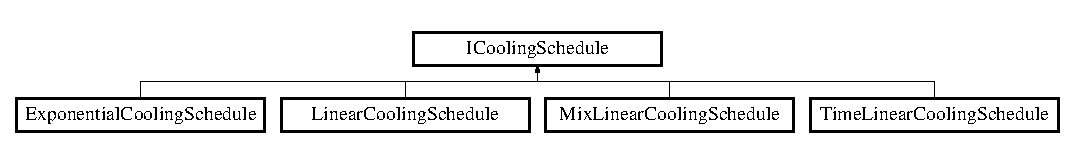
\includegraphics[height=1.546961cm]{classICoolingSchedule}
\end{center}
\end{figure}
\subsection*{\-Public \-Member \-Functions}
\begin{DoxyCompactItemize}
\item 
virtual double \hyperlink{classICoolingSchedule_ac5d2dbf784cde3a36fd5e7c5c3fbdd96}{get\-Current\-Temperature} ()=0
\item 
virtual void \hyperlink{classICoolingSchedule_aa87b9fe07eb7f03a7c4bad8f6f31b8a2}{start\-Signal} ()
\end{DoxyCompactItemize}


\subsection{\-Detailed \-Description}
\-This is an interface to define cooling schedule to be used by a simulated annealing. 

\subsection{\-Member \-Function \-Documentation}
\hypertarget{classICoolingSchedule_ac5d2dbf784cde3a36fd5e7c5c3fbdd96}{\index{\-I\-Cooling\-Schedule@{\-I\-Cooling\-Schedule}!get\-Current\-Temperature@{get\-Current\-Temperature}}
\index{get\-Current\-Temperature@{get\-Current\-Temperature}!ICoolingSchedule@{\-I\-Cooling\-Schedule}}
\subsubsection[{get\-Current\-Temperature}]{\setlength{\rightskip}{0pt plus 5cm}virtual double {\bf \-I\-Cooling\-Schedule\-::get\-Current\-Temperature} (
\begin{DoxyParamCaption}
{}
\end{DoxyParamCaption}
)\hspace{0.3cm}{\ttfamily  \mbox{[}pure virtual\mbox{]}}}}\label{classICoolingSchedule_ac5d2dbf784cde3a36fd5e7c5c3fbdd96}
\begin{DoxyReturn}{\-Returns}
the current temperature. 
\end{DoxyReturn}


\-Implemented in \hyperlink{classLinearCoolingSchedule_ab47b31f34bfe387e9c70d702a0b6301b}{\-Linear\-Cooling\-Schedule}, \hyperlink{classExponentialCoolingSchedule_ac32efff552a53ff64ff00deb490b1cb7}{\-Exponential\-Cooling\-Schedule}, \hyperlink{classMixLinearCoolingSchedule_aa388d2510df3ae9eff98bc48df8dc92d}{\-Mix\-Linear\-Cooling\-Schedule}, and \hyperlink{classTimeLinearCoolingSchedule_a67dffb918e6c67ba8fecad1b764f36ea}{\-Time\-Linear\-Cooling\-Schedule}.

\hypertarget{classICoolingSchedule_aa87b9fe07eb7f03a7c4bad8f6f31b8a2}{\index{\-I\-Cooling\-Schedule@{\-I\-Cooling\-Schedule}!start\-Signal@{start\-Signal}}
\index{start\-Signal@{start\-Signal}!ICoolingSchedule@{\-I\-Cooling\-Schedule}}
\subsubsection[{start\-Signal}]{\setlength{\rightskip}{0pt plus 5cm}virtual void {\bf \-I\-Cooling\-Schedule\-::start\-Signal} (
\begin{DoxyParamCaption}
{}
\end{DoxyParamCaption}
)\hspace{0.3cm}{\ttfamily  \mbox{[}inline, virtual\mbox{]}}}}\label{classICoolingSchedule_aa87b9fe07eb7f03a7c4bad8f6f31b8a2}
\-This method should be called when the optimization process start. \-The cooling schedules that actually need this should override this method. 

\-Reimplemented in \hyperlink{classLinearCoolingSchedule_a384afd4b7b7e89ebf1268974b28fad84}{\-Linear\-Cooling\-Schedule}, \hyperlink{classExponentialCoolingSchedule_a64b6a3c4b329b18ca55c68d75cb03a00}{\-Exponential\-Cooling\-Schedule}, \hyperlink{classMixLinearCoolingSchedule_a97c3c7d9e485ee6d1ee5cd19175f56b7}{\-Mix\-Linear\-Cooling\-Schedule}, and \hyperlink{classTimeLinearCoolingSchedule_a44190e4c27b218610724a8e41c65291f}{\-Time\-Linear\-Cooling\-Schedule}.



\-The documentation for this class was generated from the following file\-:\begin{DoxyCompactItemize}
\item 
\-A\-L\-N\-S\-\_\-\-Static\-\_\-\-Lib/src/acceptance\-Module/\-I\-Cooling\-Schedule.\-h\end{DoxyCompactItemize}

\hypertarget{classILocalSearch}{\section{\-I\-Local\-Search \-Class \-Reference}
\label{classILocalSearch}\index{\-I\-Local\-Search@{\-I\-Local\-Search}}
}
\subsection*{\-Public \-Member \-Functions}
\begin{DoxyCompactItemize}
\item 
virtual bool \hyperlink{classILocalSearch_a90d10a19f474467638bbafbe702cd321}{perform\-Local\-Search} (\hyperlink{classISolution}{\-I\-Solution} \&sol)=0
\item 
virtual std\-::string \hyperlink{classILocalSearch_a9f65ab48fd9feae07a4314544908bbe7}{get\-Name} ()=0
\end{DoxyCompactItemize}


\subsection{\-Member \-Function \-Documentation}
\hypertarget{classILocalSearch_a9f65ab48fd9feae07a4314544908bbe7}{\index{\-I\-Local\-Search@{\-I\-Local\-Search}!get\-Name@{get\-Name}}
\index{get\-Name@{get\-Name}!ILocalSearch@{\-I\-Local\-Search}}
\subsubsection[{get\-Name}]{\setlength{\rightskip}{0pt plus 5cm}virtual std\-::string {\bf \-I\-Local\-Search\-::get\-Name} (
\begin{DoxyParamCaption}
{}
\end{DoxyParamCaption}
)\hspace{0.3cm}{\ttfamily  \mbox{[}pure virtual\mbox{]}}}}\label{classILocalSearch_a9f65ab48fd9feae07a4314544908bbe7}
\begin{DoxyReturn}{\-Returns}
the name of the local search operator. 
\end{DoxyReturn}
\hypertarget{classILocalSearch_a90d10a19f474467638bbafbe702cd321}{\index{\-I\-Local\-Search@{\-I\-Local\-Search}!perform\-Local\-Search@{perform\-Local\-Search}}
\index{perform\-Local\-Search@{perform\-Local\-Search}!ILocalSearch@{\-I\-Local\-Search}}
\subsubsection[{perform\-Local\-Search}]{\setlength{\rightskip}{0pt plus 5cm}virtual bool {\bf \-I\-Local\-Search\-::perform\-Local\-Search} (
\begin{DoxyParamCaption}
\item[{{\bf \-I\-Solution} \&}]{sol}
\end{DoxyParamCaption}
)\hspace{0.3cm}{\ttfamily  \mbox{[}pure virtual\mbox{]}}}}\label{classILocalSearch_a90d10a19f474467638bbafbe702cd321}
\-Perform a local search on the solution. \begin{DoxyReturn}{\-Returns}
true if the solution is improved. 
\end{DoxyReturn}


\-The documentation for this class was generated from the following file\-:\begin{DoxyCompactItemize}
\item 
\-A\-L\-N\-S\-\_\-\-Static\-\_\-\-Lib/src/localsearch/\-I\-Local\-Search.\-h\end{DoxyCompactItemize}

\hypertarget{classILocalSearchManager}{\section{\-I\-Local\-Search\-Manager \-Class \-Reference}
\label{classILocalSearchManager}\index{\-I\-Local\-Search\-Manager@{\-I\-Local\-Search\-Manager}}
}
\-Inheritance diagram for \-I\-Local\-Search\-Manager\-:\begin{figure}[H]
\begin{center}
\leavevmode
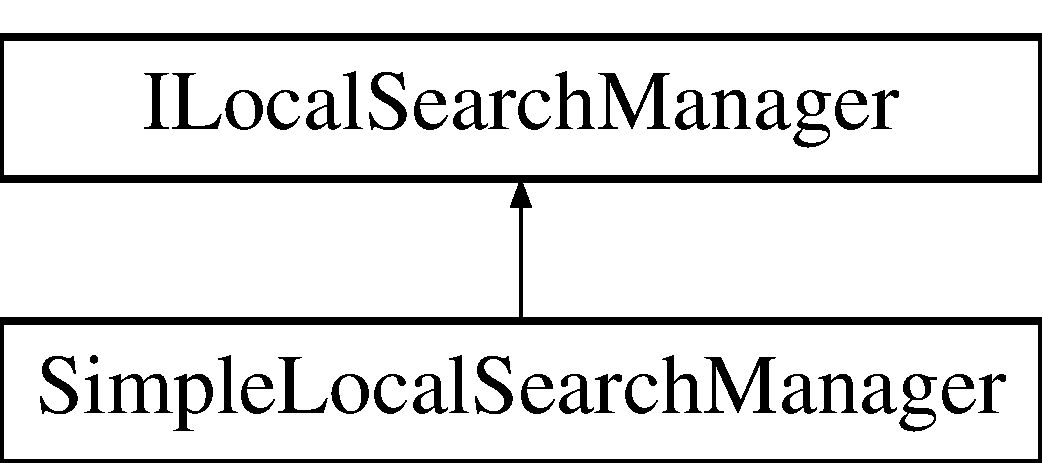
\includegraphics[height=2.000000cm]{classILocalSearchManager}
\end{center}
\end{figure}
\subsection*{\-Public \-Member \-Functions}
\begin{DoxyCompactItemize}
\item 
virtual bool \hyperlink{classILocalSearchManager_ab12f478c7be7163b674374ba478f2cbd}{use\-Local\-Search} (\hyperlink{classISolution}{\-I\-Solution} \&sol, \hyperlink{classALNS__Iteration__Status}{\-A\-L\-N\-S\-\_\-\-Iteration\-\_\-\-Status} \&status)=0
\item 
\hypertarget{classILocalSearchManager_a8a4ff2fd07e7ac3a81eb55e4482f6cf6}{virtual void \hyperlink{classILocalSearchManager_a8a4ff2fd07e7ac3a81eb55e4482f6cf6}{start\-Signal} ()=0}\label{classILocalSearchManager_a8a4ff2fd07e7ac3a81eb55e4482f6cf6}

\begin{DoxyCompactList}\small\item\em \-Indicate that the optimization process starts. \end{DoxyCompactList}\end{DoxyCompactItemize}


\subsection{\-Member \-Function \-Documentation}
\hypertarget{classILocalSearchManager_ab12f478c7be7163b674374ba478f2cbd}{\index{\-I\-Local\-Search\-Manager@{\-I\-Local\-Search\-Manager}!use\-Local\-Search@{use\-Local\-Search}}
\index{use\-Local\-Search@{use\-Local\-Search}!ILocalSearchManager@{\-I\-Local\-Search\-Manager}}
\subsubsection[{use\-Local\-Search}]{\setlength{\rightskip}{0pt plus 5cm}virtual bool {\bf \-I\-Local\-Search\-Manager\-::use\-Local\-Search} (
\begin{DoxyParamCaption}
\item[{{\bf \-I\-Solution} \&}]{sol, }
\item[{{\bf \-A\-L\-N\-S\-\_\-\-Iteration\-\_\-\-Status} \&}]{status}
\end{DoxyParamCaption}
)\hspace{0.3cm}{\ttfamily  \mbox{[}pure virtual\mbox{]}}}}\label{classILocalSearchManager_ab12f478c7be7163b674374ba478f2cbd}

\begin{DoxyParams}{\-Parameters}
{\em sol} & the solution to be improved. \\
\hline
{\em status} & the status of the alns iteration. \\
\hline
\end{DoxyParams}
\begin{DoxyReturn}{\-Returns}
true if the solution has been improved. 
\end{DoxyReturn}


\-Implemented in \hyperlink{classSimpleLocalSearchManager_a213c380b351e4c7c4b4948ad7da513a7}{\-Simple\-Local\-Search\-Manager}.



\-The documentation for this class was generated from the following file\-:\begin{DoxyCompactItemize}
\item 
\-A\-L\-N\-S\-\_\-\-Static\-\_\-\-Lib/src/localsearch/\-I\-Local\-Search\-Manager.\-h\end{DoxyCompactItemize}

\hypertarget{classIOperatorManager}{\section{\-I\-Operator\-Manager \-Class \-Reference}
\label{classIOperatorManager}\index{\-I\-Operator\-Manager@{\-I\-Operator\-Manager}}
}


\-This interface represent the methods that should be implemented by an operator manager.  




{\ttfamily \#include $<$\-A\-Operator\-Manager.\-h$>$}



\subsection{\-Detailed \-Description}
\-This interface represent the methods that should be implemented by an operator manager. 

\-The documentation for this class was generated from the following file\-:\begin{DoxyCompactItemize}
\item 
\-A\-L\-N\-S\-\_\-\-Static\-\_\-\-Lib/src/alns/\-A\-Operator\-Manager.\-h\end{DoxyCompactItemize}

\hypertarget{classISolution}{\section{\-I\-Solution \-Class \-Reference}
\label{classISolution}\index{\-I\-Solution@{\-I\-Solution}}
}


\-An interface to define \-Solutions.  




{\ttfamily \#include $<$\-I\-Solution.\-h$>$}

\subsection*{\-Public \-Member \-Functions}
\begin{DoxyCompactItemize}
\item 
virtual double \hyperlink{classISolution_a364e6cf3ee78b16b4b78d1a5612c5e70}{get\-Objective\-Value} ()=0
\item 
virtual double \hyperlink{classISolution_a577a02712a4e973a5acda9926d025afb}{get\-Penalized\-Objective\-Value} ()=0
\item 
virtual bool \hyperlink{classISolution_a4619382420ff245fcf12465557587ee6}{is\-Feasible} ()=0
\item 
virtual bool \hyperlink{classISolution_a9293d9e9eb00bab08dc25d11c61a1410}{operator$<$} (\hyperlink{classISolution}{\-I\-Solution} \&)=0
\item 
virtual int \hyperlink{classISolution_a60ba3056f6733fa50260466f3eb89a21}{distance} (\hyperlink{classISolution}{\-I\-Solution} \&)=0
\item 
\hypertarget{classISolution_accb0408d64b7e06f48054708eca34101}{virtual \hyperlink{classISolution}{\-I\-Solution} $\ast$ \hyperlink{classISolution_accb0408d64b7e06f48054708eca34101}{get\-Copy} ()=0}\label{classISolution_accb0408d64b7e06f48054708eca34101}

\begin{DoxyCompactList}\small\item\em \-This method create a copy of the solution. \end{DoxyCompactList}\item 
\hypertarget{classISolution_a5a3e735aab6b276f1f4da959442ffad6}{virtual long long \hyperlink{classISolution_a5a3e735aab6b276f1f4da959442ffad6}{get\-Hash} ()=0}\label{classISolution_a5a3e735aab6b276f1f4da959442ffad6}

\begin{DoxyCompactList}\small\item\em \-Compute a hash key of the solution. \end{DoxyCompactList}\end{DoxyCompactItemize}


\subsection{\-Detailed \-Description}
\-An interface to define \-Solutions. 

\subsection{\-Member \-Function \-Documentation}
\hypertarget{classISolution_a60ba3056f6733fa50260466f3eb89a21}{\index{\-I\-Solution@{\-I\-Solution}!distance@{distance}}
\index{distance@{distance}!ISolution@{\-I\-Solution}}
\subsubsection[{distance}]{\setlength{\rightskip}{0pt plus 5cm}virtual int {\bf \-I\-Solution\-::distance} (
\begin{DoxyParamCaption}
\item[{{\bf \-I\-Solution} \&}]{}
\end{DoxyParamCaption}
)\hspace{0.3cm}{\ttfamily  \mbox{[}pure virtual\mbox{]}}}}\label{classISolution_a60ba3056f6733fa50260466f3eb89a21}
\-Compute the \char`\"{}distance\char`\"{} between solution. \-This feature can be used as part of the \hyperlink{classALNS}{\-A\-L\-N\-S} to favor the diversification process. \-If you do not plan to use this feature just implement a method returning 0. \hypertarget{classISolution_a364e6cf3ee78b16b4b78d1a5612c5e70}{\index{\-I\-Solution@{\-I\-Solution}!get\-Objective\-Value@{get\-Objective\-Value}}
\index{get\-Objective\-Value@{get\-Objective\-Value}!ISolution@{\-I\-Solution}}
\subsubsection[{get\-Objective\-Value}]{\setlength{\rightskip}{0pt plus 5cm}virtual double {\bf \-I\-Solution\-::get\-Objective\-Value} (
\begin{DoxyParamCaption}
{}
\end{DoxyParamCaption}
)\hspace{0.3cm}{\ttfamily  \mbox{[}pure virtual\mbox{]}}}}\label{classISolution_a364e6cf3ee78b16b4b78d1a5612c5e70}
\-A getter for the value of the objective function. \begin{DoxyReturn}{\-Returns}
the value of the objective function of this solution. 
\end{DoxyReturn}
\hypertarget{classISolution_a577a02712a4e973a5acda9926d025afb}{\index{\-I\-Solution@{\-I\-Solution}!get\-Penalized\-Objective\-Value@{get\-Penalized\-Objective\-Value}}
\index{get\-Penalized\-Objective\-Value@{get\-Penalized\-Objective\-Value}!ISolution@{\-I\-Solution}}
\subsubsection[{get\-Penalized\-Objective\-Value}]{\setlength{\rightskip}{0pt plus 5cm}virtual double {\bf \-I\-Solution\-::get\-Penalized\-Objective\-Value} (
\begin{DoxyParamCaption}
{}
\end{DoxyParamCaption}
)\hspace{0.3cm}{\ttfamily  \mbox{[}pure virtual\mbox{]}}}}\label{classISolution_a577a02712a4e973a5acda9926d025afb}
\begin{DoxyReturn}{\-Returns}
a penalized version of the objective value if the solution is infeasible. 
\end{DoxyReturn}
\hypertarget{classISolution_a4619382420ff245fcf12465557587ee6}{\index{\-I\-Solution@{\-I\-Solution}!is\-Feasible@{is\-Feasible}}
\index{is\-Feasible@{is\-Feasible}!ISolution@{\-I\-Solution}}
\subsubsection[{is\-Feasible}]{\setlength{\rightskip}{0pt plus 5cm}virtual bool {\bf \-I\-Solution\-::is\-Feasible} (
\begin{DoxyParamCaption}
{}
\end{DoxyParamCaption}
)\hspace{0.3cm}{\ttfamily  \mbox{[}pure virtual\mbox{]}}}}\label{classISolution_a4619382420ff245fcf12465557587ee6}
\-A getter for the feasibility of the current solution. \begin{DoxyReturn}{\-Returns}
true if the solution is feasible, false otherwise. 
\end{DoxyReturn}
\hypertarget{classISolution_a9293d9e9eb00bab08dc25d11c61a1410}{\index{\-I\-Solution@{\-I\-Solution}!operator$<$@{operator$<$}}
\index{operator$<$@{operator$<$}!ISolution@{\-I\-Solution}}
\subsubsection[{operator$<$}]{\setlength{\rightskip}{0pt plus 5cm}virtual bool \-I\-Solution\-::operator$<$ (
\begin{DoxyParamCaption}
\item[{{\bf \-I\-Solution} \&}]{}
\end{DoxyParamCaption}
)\hspace{0.3cm}{\ttfamily  \mbox{[}pure virtual\mbox{]}}}}\label{classISolution_a9293d9e9eb00bab08dc25d11c61a1410}
\-A comparator. \begin{DoxyReturn}{\-Returns}
true if this solution is \char`\"{}better\char`\"{} than the solution it is compared to. 
\end{DoxyReturn}


\-The documentation for this class was generated from the following file\-:\begin{DoxyCompactItemize}
\item 
\-A\-L\-N\-S\-\_\-\-Static\-\_\-\-Lib/src/alns/\-I\-Solution.\-h\end{DoxyCompactItemize}

\hypertarget{classIUpdatable}{\section{\-I\-Updatable \-Class \-Reference}
\label{classIUpdatable}\index{\-I\-Updatable@{\-I\-Updatable}}
}


\-An interface define object that should be updated using solution information or iteration status information.  




{\ttfamily \#include $<$\-I\-Updatable.\-h$>$}

\subsection*{\-Public \-Member \-Functions}
\begin{DoxyCompactItemize}
\item 
\hypertarget{classIUpdatable_a827ad7762d82343eb1fa07406e74951c}{virtual void {\bfseries update} (\hyperlink{classISolution}{\-I\-Solution} \&sol, \hyperlink{classALNS__Iteration__Status}{\-A\-L\-N\-S\-\_\-\-Iteration\-\_\-\-Status} \&status)=0}\label{classIUpdatable_a827ad7762d82343eb1fa07406e74951c}

\end{DoxyCompactItemize}


\subsection{\-Detailed \-Description}
\-An interface define object that should be updated using solution information or iteration status information. 

\-The documentation for this class was generated from the following file\-:\begin{DoxyCompactItemize}
\item 
\-A\-L\-N\-S\-\_\-\-Static\-\_\-\-Lib/src/alns/\-I\-Updatable.\-h\end{DoxyCompactItemize}

\hypertarget{classLinearCoolingSchedule}{\section{\-Linear\-Cooling\-Schedule \-Class \-Reference}
\label{classLinearCoolingSchedule}\index{\-Linear\-Cooling\-Schedule@{\-Linear\-Cooling\-Schedule}}
}


\-A linear cooling schedule based on the total number of iterations.  




{\ttfamily \#include $<$\-Linear\-Cooling\-Schedule.\-h$>$}

\-Inheritance diagram for \-Linear\-Cooling\-Schedule\-:\begin{figure}[H]
\begin{center}
\leavevmode
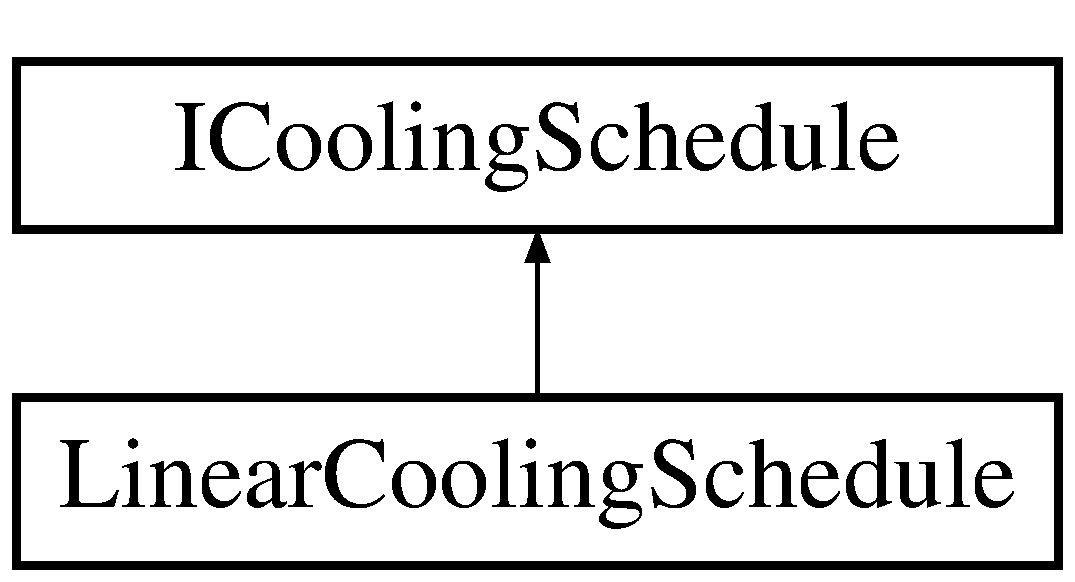
\includegraphics[height=2.000000cm]{classLinearCoolingSchedule}
\end{center}
\end{figure}
\subsection*{\-Public \-Member \-Functions}
\begin{DoxyCompactItemize}
\item 
\hyperlink{classLinearCoolingSchedule_a160016c6d7f09872a5c78a407d502085}{\-Linear\-Cooling\-Schedule} (\hyperlink{classISolution}{\-I\-Solution} \&init\-Sol, \hyperlink{classCoolingSchedule__Parameters}{\-Cooling\-Schedule\-\_\-\-Parameters} \&cs\-Param, size\-\_\-t nb\-Iterations)
\item 
\hyperlink{classLinearCoolingSchedule_aa581bf5d7b74d60784050a6d857dccf6}{\-Linear\-Cooling\-Schedule} (double starting\-Temperature, size\-\_\-t nb\-Iterations)
\item 
\hypertarget{classLinearCoolingSchedule_a81dba7fe99429e38ec03b865d897e1b9}{virtual \hyperlink{classLinearCoolingSchedule_a81dba7fe99429e38ec03b865d897e1b9}{$\sim$\-Linear\-Cooling\-Schedule} ()}\label{classLinearCoolingSchedule_a81dba7fe99429e38ec03b865d897e1b9}

\begin{DoxyCompactList}\small\item\em \-Destructor. \end{DoxyCompactList}\item 
double \hyperlink{classLinearCoolingSchedule_ab47b31f34bfe387e9c70d702a0b6301b}{get\-Current\-Temperature} ()
\item 
void \hyperlink{classLinearCoolingSchedule_a384afd4b7b7e89ebf1268974b28fad84}{start\-Signal} ()
\end{DoxyCompactItemize}


\subsection{\-Detailed \-Description}
\-A linear cooling schedule based on the total number of iterations. 

\subsection{\-Constructor \& \-Destructor \-Documentation}
\hypertarget{classLinearCoolingSchedule_a160016c6d7f09872a5c78a407d502085}{\index{\-Linear\-Cooling\-Schedule@{\-Linear\-Cooling\-Schedule}!\-Linear\-Cooling\-Schedule@{\-Linear\-Cooling\-Schedule}}
\index{\-Linear\-Cooling\-Schedule@{\-Linear\-Cooling\-Schedule}!LinearCoolingSchedule@{\-Linear\-Cooling\-Schedule}}
\subsubsection[{\-Linear\-Cooling\-Schedule}]{\setlength{\rightskip}{0pt plus 5cm}{\bf \-Linear\-Cooling\-Schedule\-::\-Linear\-Cooling\-Schedule} (
\begin{DoxyParamCaption}
\item[{{\bf \-I\-Solution} \&}]{init\-Sol, }
\item[{{\bf \-Cooling\-Schedule\-\_\-\-Parameters} \&}]{cs\-Param, }
\item[{size\-\_\-t}]{nb\-Iterations}
\end{DoxyParamCaption}
)}}\label{classLinearCoolingSchedule_a160016c6d7f09872a5c78a407d502085}
\-Constructor. 
\begin{DoxyParams}{\-Parameters}
{\em init\-Sol} & the initial solution. \\
\hline
{\em cs\-Param} & the cooling schedule parameters. \\
\hline
{\em nb\-Iterations} & the number of iterations to be performed. \\
\hline
\end{DoxyParams}
\hypertarget{classLinearCoolingSchedule_aa581bf5d7b74d60784050a6d857dccf6}{\index{\-Linear\-Cooling\-Schedule@{\-Linear\-Cooling\-Schedule}!\-Linear\-Cooling\-Schedule@{\-Linear\-Cooling\-Schedule}}
\index{\-Linear\-Cooling\-Schedule@{\-Linear\-Cooling\-Schedule}!LinearCoolingSchedule@{\-Linear\-Cooling\-Schedule}}
\subsubsection[{\-Linear\-Cooling\-Schedule}]{\setlength{\rightskip}{0pt plus 5cm}{\bf \-Linear\-Cooling\-Schedule\-::\-Linear\-Cooling\-Schedule} (
\begin{DoxyParamCaption}
\item[{double}]{starting\-Temperature, }
\item[{size\-\_\-t}]{nb\-Iterations}
\end{DoxyParamCaption}
)}}\label{classLinearCoolingSchedule_aa581bf5d7b74d60784050a6d857dccf6}
\-Constructor. 
\begin{DoxyParams}{\-Parameters}
{\em starting\-Temperature} & the initial temperature. \\
\hline
{\em nb\-Iterations} & the number of iterations to be performed. \\
\hline
\end{DoxyParams}


\subsection{\-Member \-Function \-Documentation}
\hypertarget{classLinearCoolingSchedule_ab47b31f34bfe387e9c70d702a0b6301b}{\index{\-Linear\-Cooling\-Schedule@{\-Linear\-Cooling\-Schedule}!get\-Current\-Temperature@{get\-Current\-Temperature}}
\index{get\-Current\-Temperature@{get\-Current\-Temperature}!LinearCoolingSchedule@{\-Linear\-Cooling\-Schedule}}
\subsubsection[{get\-Current\-Temperature}]{\setlength{\rightskip}{0pt plus 5cm}double {\bf \-Linear\-Cooling\-Schedule\-::get\-Current\-Temperature} (
\begin{DoxyParamCaption}
{}
\end{DoxyParamCaption}
)\hspace{0.3cm}{\ttfamily  \mbox{[}virtual\mbox{]}}}}\label{classLinearCoolingSchedule_ab47b31f34bfe387e9c70d702a0b6301b}
\-Compute and return the current temperature. \begin{DoxyReturn}{\-Returns}
the current temperature. 
\end{DoxyReturn}


\-Implements \hyperlink{classICoolingSchedule_ac5d2dbf784cde3a36fd5e7c5c3fbdd96}{\-I\-Cooling\-Schedule}.

\hypertarget{classLinearCoolingSchedule_a384afd4b7b7e89ebf1268974b28fad84}{\index{\-Linear\-Cooling\-Schedule@{\-Linear\-Cooling\-Schedule}!start\-Signal@{start\-Signal}}
\index{start\-Signal@{start\-Signal}!LinearCoolingSchedule@{\-Linear\-Cooling\-Schedule}}
\subsubsection[{start\-Signal}]{\setlength{\rightskip}{0pt plus 5cm}void {\bf \-Linear\-Cooling\-Schedule\-::start\-Signal} (
\begin{DoxyParamCaption}
{}
\end{DoxyParamCaption}
)\hspace{0.3cm}{\ttfamily  \mbox{[}inline, virtual\mbox{]}}}}\label{classLinearCoolingSchedule_a384afd4b7b7e89ebf1268974b28fad84}
\-This method should be called when the optimization process start. \-The cooling schedules that actually need this should override this method. 

\-Reimplemented from \hyperlink{classICoolingSchedule_aa87b9fe07eb7f03a7c4bad8f6f31b8a2}{\-I\-Cooling\-Schedule}.



\-The documentation for this class was generated from the following files\-:\begin{DoxyCompactItemize}
\item 
\-A\-L\-N\-S\-\_\-\-Static\-\_\-\-Lib/src/acceptance\-Module/\-Linear\-Cooling\-Schedule.\-h\item 
\-A\-L\-N\-S\-\_\-\-Static\-\_\-\-Lib/src/acceptance\-Module/\-Linear\-Cooling\-Schedule.\-cpp\end{DoxyCompactItemize}

\hypertarget{classMixLinearCoolingSchedule}{\section{\-Mix\-Linear\-Cooling\-Schedule \-Class \-Reference}
\label{classMixLinearCoolingSchedule}\index{\-Mix\-Linear\-Cooling\-Schedule@{\-Mix\-Linear\-Cooling\-Schedule}}
}


\-A linear cooling schedule based on a mix of the total number of iterations and the maximum running time.  




{\ttfamily \#include $<$\-Mix\-Linear\-Cooling\-Schedule.\-h$>$}

\-Inheritance diagram for \-Mix\-Linear\-Cooling\-Schedule\-:\begin{figure}[H]
\begin{center}
\leavevmode
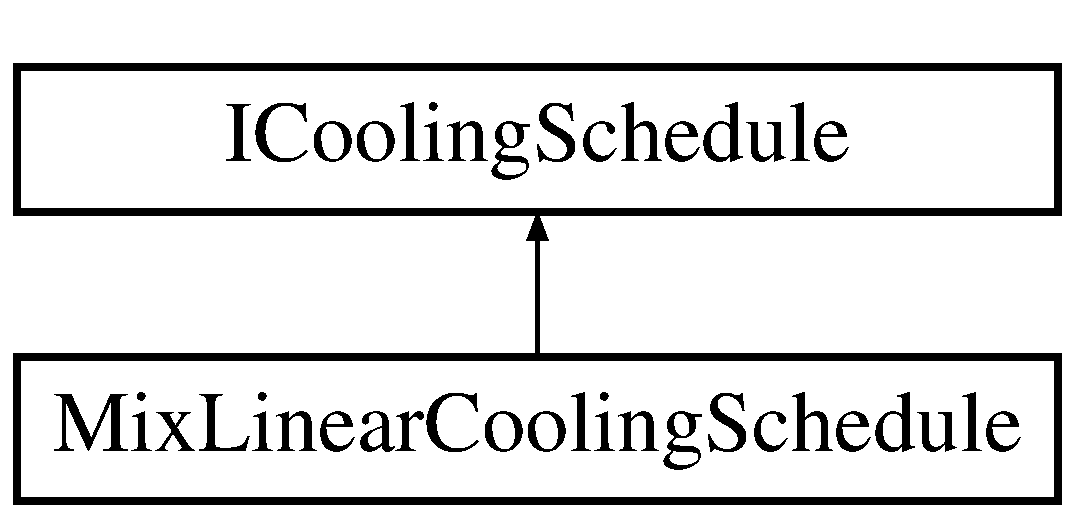
\includegraphics[height=2.000000cm]{classMixLinearCoolingSchedule}
\end{center}
\end{figure}
\subsection*{\-Public \-Member \-Functions}
\begin{DoxyCompactItemize}
\item 
\hyperlink{classMixLinearCoolingSchedule_a251ce5ccff60cfba8ce6121cbbb0e7f2}{\-Mix\-Linear\-Cooling\-Schedule} (\hyperlink{classISolution}{\-I\-Solution} \&init\-Sol, \hyperlink{classCoolingSchedule__Parameters}{\-Cooling\-Schedule\-\_\-\-Parameters} \&cs\-Param)
\item 
\hypertarget{classMixLinearCoolingSchedule_a97e65c5d3b320123218bef961a1b0b25}{virtual \hyperlink{classMixLinearCoolingSchedule_a97e65c5d3b320123218bef961a1b0b25}{$\sim$\-Mix\-Linear\-Cooling\-Schedule} ()}\label{classMixLinearCoolingSchedule_a97e65c5d3b320123218bef961a1b0b25}

\begin{DoxyCompactList}\small\item\em \-Destructor. \end{DoxyCompactList}\item 
double \hyperlink{classMixLinearCoolingSchedule_aa388d2510df3ae9eff98bc48df8dc92d}{get\-Current\-Temperature} ()
\item 
virtual void \hyperlink{classMixLinearCoolingSchedule_a97c3c7d9e485ee6d1ee5cd19175f56b7}{start\-Signal} ()
\end{DoxyCompactItemize}


\subsection{\-Detailed \-Description}
\-A linear cooling schedule based on a mix of the total number of iterations and the maximum running time. 

\subsection{\-Constructor \& \-Destructor \-Documentation}
\hypertarget{classMixLinearCoolingSchedule_a251ce5ccff60cfba8ce6121cbbb0e7f2}{\index{\-Mix\-Linear\-Cooling\-Schedule@{\-Mix\-Linear\-Cooling\-Schedule}!\-Mix\-Linear\-Cooling\-Schedule@{\-Mix\-Linear\-Cooling\-Schedule}}
\index{\-Mix\-Linear\-Cooling\-Schedule@{\-Mix\-Linear\-Cooling\-Schedule}!MixLinearCoolingSchedule@{\-Mix\-Linear\-Cooling\-Schedule}}
\subsubsection[{\-Mix\-Linear\-Cooling\-Schedule}]{\setlength{\rightskip}{0pt plus 5cm}{\bf \-Mix\-Linear\-Cooling\-Schedule\-::\-Mix\-Linear\-Cooling\-Schedule} (
\begin{DoxyParamCaption}
\item[{{\bf \-I\-Solution} \&}]{init\-Sol, }
\item[{{\bf \-Cooling\-Schedule\-\_\-\-Parameters} \&}]{cs\-Param}
\end{DoxyParamCaption}
)}}\label{classMixLinearCoolingSchedule_a251ce5ccff60cfba8ce6121cbbb0e7f2}
\-Constructor. 
\begin{DoxyParams}{\-Parameters}
{\em init\-Sol} & the initial solution. \\
\hline
{\em cs\-Param} & the cooling schedule parameters to be used. \\
\hline
\end{DoxyParams}


\subsection{\-Member \-Function \-Documentation}
\hypertarget{classMixLinearCoolingSchedule_aa388d2510df3ae9eff98bc48df8dc92d}{\index{\-Mix\-Linear\-Cooling\-Schedule@{\-Mix\-Linear\-Cooling\-Schedule}!get\-Current\-Temperature@{get\-Current\-Temperature}}
\index{get\-Current\-Temperature@{get\-Current\-Temperature}!MixLinearCoolingSchedule@{\-Mix\-Linear\-Cooling\-Schedule}}
\subsubsection[{get\-Current\-Temperature}]{\setlength{\rightskip}{0pt plus 5cm}double {\bf \-Mix\-Linear\-Cooling\-Schedule\-::get\-Current\-Temperature} (
\begin{DoxyParamCaption}
{}
\end{DoxyParamCaption}
)\hspace{0.3cm}{\ttfamily  \mbox{[}virtual\mbox{]}}}}\label{classMixLinearCoolingSchedule_aa388d2510df3ae9eff98bc48df8dc92d}
\-Compute and return the current temperature. \begin{DoxyReturn}{\-Returns}
the current temperature. 
\end{DoxyReturn}


\-Implements \hyperlink{classICoolingSchedule_ac5d2dbf784cde3a36fd5e7c5c3fbdd96}{\-I\-Cooling\-Schedule}.

\hypertarget{classMixLinearCoolingSchedule_a97c3c7d9e485ee6d1ee5cd19175f56b7}{\index{\-Mix\-Linear\-Cooling\-Schedule@{\-Mix\-Linear\-Cooling\-Schedule}!start\-Signal@{start\-Signal}}
\index{start\-Signal@{start\-Signal}!MixLinearCoolingSchedule@{\-Mix\-Linear\-Cooling\-Schedule}}
\subsubsection[{start\-Signal}]{\setlength{\rightskip}{0pt plus 5cm}void {\bf \-Mix\-Linear\-Cooling\-Schedule\-::start\-Signal} (
\begin{DoxyParamCaption}
{}
\end{DoxyParamCaption}
)\hspace{0.3cm}{\ttfamily  \mbox{[}virtual\mbox{]}}}}\label{classMixLinearCoolingSchedule_a97c3c7d9e485ee6d1ee5cd19175f56b7}
\-This method should be called when the optimization process start. \-The cooling schedules that actually need this should override this method. 

\-Reimplemented from \hyperlink{classICoolingSchedule_aa87b9fe07eb7f03a7c4bad8f6f31b8a2}{\-I\-Cooling\-Schedule}.



\-The documentation for this class was generated from the following files\-:\begin{DoxyCompactItemize}
\item 
\-A\-L\-N\-S\-\_\-\-Static\-\_\-\-Lib/src/acceptance\-Module/\-Mix\-Linear\-Cooling\-Schedule.\-h\item 
\-A\-L\-N\-S\-\_\-\-Static\-\_\-\-Lib/src/acceptance\-Module/\-Mix\-Linear\-Cooling\-Schedule.\-cpp\end{DoxyCompactItemize}

\hypertarget{classOperatorManager}{\section{\-Operator\-Manager \-Class \-Reference}
\label{classOperatorManager}\index{\-Operator\-Manager@{\-Operator\-Manager}}
}


\-A simple implementation of an operator manager, that does not allow to simply couple the destroy and repair operators.  




{\ttfamily \#include $<$\-Operator\-Manager.\-h$>$}

\-Inheritance diagram for \-Operator\-Manager\-:\begin{figure}[H]
\begin{center}
\leavevmode
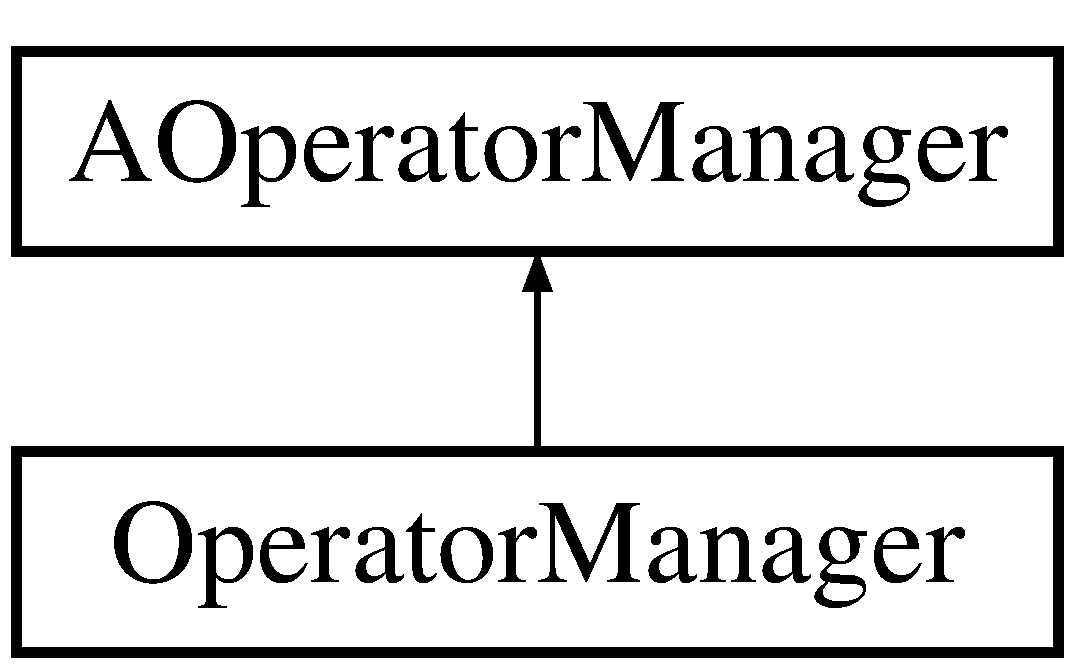
\includegraphics[height=2.000000cm]{classOperatorManager}
\end{center}
\end{figure}
\subsection*{\-Public \-Member \-Functions}
\begin{DoxyCompactItemize}
\item 
\hyperlink{classOperatorManager_ae4f84de6b7812b951ee202e8c2afe478}{\-Operator\-Manager} (\hyperlink{classALNS__Parameters}{\-A\-L\-N\-S\-\_\-\-Parameters} \&param)
\item 
\hypertarget{classOperatorManager_ad0b56a48c3e5ccb422f8944bcd3dce6d}{virtual \hyperlink{classOperatorManager_ad0b56a48c3e5ccb422f8944bcd3dce6d}{$\sim$\-Operator\-Manager} ()}\label{classOperatorManager_ad0b56a48c3e5ccb422f8944bcd3dce6d}

\begin{DoxyCompactList}\small\item\em \-Destructor. \end{DoxyCompactList}\item 
void \hyperlink{classOperatorManager_afcd6148f23aa4faae18bc5b8a08cbd20}{recompute\-Weights} ()
\item 
\hyperlink{classADestroyOperator}{\-A\-Destroy\-Operator} \& \hyperlink{classOperatorManager_ae2b34fa76d49119d61836db181890085}{select\-Destroy\-Operator} ()
\item 
\hyperlink{classARepairOperator}{\-A\-Repair\-Operator} \& \hyperlink{classOperatorManager_a620514b4b09095e5533e2fe3a44df529}{select\-Repair\-Operator} ()
\item 
void \hyperlink{classOperatorManager_a4bbeee23953420b0be2d6a72388e75e9}{add\-Repair\-Operator} (\hyperlink{classARepairOperator}{\-A\-Repair\-Operator} \&repair\-Operator)
\item 
void \hyperlink{classOperatorManager_a5760dee74c37a6d5e3fea78250afbd69}{add\-Destroy\-Operator} (\hyperlink{classADestroyOperator}{\-A\-Destroy\-Operator} \&destroy\-Operator)
\item 
void \hyperlink{classOperatorManager_a7313370bb35e71f7a70e770c4f1f8c14}{sanity\-Checks} ()
\item 
\hypertarget{classOperatorManager_a06445bfd3151e3dfa51b06ab1664a7c7}{virtual void \hyperlink{classOperatorManager_a06445bfd3151e3dfa51b06ab1664a7c7}{update\-Scores} (\hyperlink{classADestroyOperator}{\-A\-Destroy\-Operator} \&des, \hyperlink{classARepairOperator}{\-A\-Repair\-Operator} \&rep, \hyperlink{classALNS__Iteration__Status}{\-A\-L\-N\-S\-\_\-\-Iteration\-\_\-\-Status} \&status)}\label{classOperatorManager_a06445bfd3151e3dfa51b06ab1664a7c7}

\begin{DoxyCompactList}\small\item\em \-Update the scores of the operators. \end{DoxyCompactList}\item 
\hypertarget{classOperatorManager_ac045229cf93bef316f3afd7a36c9a185}{virtual void \hyperlink{classOperatorManager_ac045229cf93bef316f3afd7a36c9a185}{start\-Signal} ()}\label{classOperatorManager_ac045229cf93bef316f3afd7a36c9a185}

\begin{DoxyCompactList}\small\item\em \-Indicate that the optimization process starts. \end{DoxyCompactList}\end{DoxyCompactItemize}


\subsection{\-Detailed \-Description}
\-A simple implementation of an operator manager, that does not allow to simply couple the destroy and repair operators. 

\subsection{\-Constructor \& \-Destructor \-Documentation}
\hypertarget{classOperatorManager_ae4f84de6b7812b951ee202e8c2afe478}{\index{\-Operator\-Manager@{\-Operator\-Manager}!\-Operator\-Manager@{\-Operator\-Manager}}
\index{\-Operator\-Manager@{\-Operator\-Manager}!OperatorManager@{\-Operator\-Manager}}
\subsubsection[{\-Operator\-Manager}]{\setlength{\rightskip}{0pt plus 5cm}{\bf \-Operator\-Manager\-::\-Operator\-Manager} (
\begin{DoxyParamCaption}
\item[{{\bf \-A\-L\-N\-S\-\_\-\-Parameters} \&}]{param}
\end{DoxyParamCaption}
)}}\label{classOperatorManager_ae4f84de6b7812b951ee202e8c2afe478}
\-Constructor 
\begin{DoxyParams}{\-Parameters}
{\em param} & the parameters to be used. \\
\hline
\end{DoxyParams}


\subsection{\-Member \-Function \-Documentation}
\hypertarget{classOperatorManager_a5760dee74c37a6d5e3fea78250afbd69}{\index{\-Operator\-Manager@{\-Operator\-Manager}!add\-Destroy\-Operator@{add\-Destroy\-Operator}}
\index{add\-Destroy\-Operator@{add\-Destroy\-Operator}!OperatorManager@{\-Operator\-Manager}}
\subsubsection[{add\-Destroy\-Operator}]{\setlength{\rightskip}{0pt plus 5cm}void {\bf \-Operator\-Manager\-::add\-Destroy\-Operator} (
\begin{DoxyParamCaption}
\item[{{\bf \-A\-Destroy\-Operator} \&}]{destroy\-Operator}
\end{DoxyParamCaption}
)}}\label{classOperatorManager_a5760dee74c37a6d5e3fea78250afbd69}
\-This method adds a destroy operator to the list of destroy operator managed by this manager. 
\begin{DoxyParams}{\-Parameters}
{\em destroy\-Operator} & the destroy operator to be added. \\
\hline
\end{DoxyParams}
\hypertarget{classOperatorManager_a4bbeee23953420b0be2d6a72388e75e9}{\index{\-Operator\-Manager@{\-Operator\-Manager}!add\-Repair\-Operator@{add\-Repair\-Operator}}
\index{add\-Repair\-Operator@{add\-Repair\-Operator}!OperatorManager@{\-Operator\-Manager}}
\subsubsection[{add\-Repair\-Operator}]{\setlength{\rightskip}{0pt plus 5cm}void {\bf \-Operator\-Manager\-::add\-Repair\-Operator} (
\begin{DoxyParamCaption}
\item[{{\bf \-A\-Repair\-Operator} \&}]{repair\-Operator}
\end{DoxyParamCaption}
)}}\label{classOperatorManager_a4bbeee23953420b0be2d6a72388e75e9}
\-This method adds a repair operator to the list of repair operator managed by this manager. 
\begin{DoxyParams}{\-Parameters}
{\em repair\-Operator} & the repair operator to be added. \\
\hline
\end{DoxyParams}
\hypertarget{classOperatorManager_afcd6148f23aa4faae18bc5b8a08cbd20}{\index{\-Operator\-Manager@{\-Operator\-Manager}!recompute\-Weights@{recompute\-Weights}}
\index{recompute\-Weights@{recompute\-Weights}!OperatorManager@{\-Operator\-Manager}}
\subsubsection[{recompute\-Weights}]{\setlength{\rightskip}{0pt plus 5cm}void {\bf \-Operator\-Manager\-::recompute\-Weights} (
\begin{DoxyParamCaption}
{}
\end{DoxyParamCaption}
)\hspace{0.3cm}{\ttfamily  \mbox{[}virtual\mbox{]}}}}\label{classOperatorManager_afcd6148f23aa4faae18bc5b8a08cbd20}
\-This function recompute the weights of every operator managed by this manager. \-Weight recomputation for destroy operators. 

\-Implements \hyperlink{classAOperatorManager}{\-A\-Operator\-Manager}.

\hypertarget{classOperatorManager_a7313370bb35e71f7a70e770c4f1f8c14}{\index{\-Operator\-Manager@{\-Operator\-Manager}!sanity\-Checks@{sanity\-Checks}}
\index{sanity\-Checks@{sanity\-Checks}!OperatorManager@{\-Operator\-Manager}}
\subsubsection[{sanity\-Checks}]{\setlength{\rightskip}{0pt plus 5cm}void {\bf \-Operator\-Manager\-::sanity\-Checks} (
\begin{DoxyParamCaption}
{}
\end{DoxyParamCaption}
)}}\label{classOperatorManager_a7313370bb35e71f7a70e770c4f1f8c14}
\-This method run some sanity checks to ensure that it is possible to \char`\"{}safely\char`\"{} use this manager within the \hyperlink{classALNS}{\-A\-L\-N\-S}. \hypertarget{classOperatorManager_ae2b34fa76d49119d61836db181890085}{\index{\-Operator\-Manager@{\-Operator\-Manager}!select\-Destroy\-Operator@{select\-Destroy\-Operator}}
\index{select\-Destroy\-Operator@{select\-Destroy\-Operator}!OperatorManager@{\-Operator\-Manager}}
\subsubsection[{select\-Destroy\-Operator}]{\setlength{\rightskip}{0pt plus 5cm}{\bf \-A\-Destroy\-Operator} \& {\bf \-Operator\-Manager\-::select\-Destroy\-Operator} (
\begin{DoxyParamCaption}
{}
\end{DoxyParamCaption}
)\hspace{0.3cm}{\ttfamily  \mbox{[}virtual\mbox{]}}}}\label{classOperatorManager_ae2b34fa76d49119d61836db181890085}
\-This method selects a destroy operator. \begin{DoxyReturn}{\-Returns}
a destroy operator. 
\end{DoxyReturn}


\-Implements \hyperlink{classAOperatorManager_a0bafced8312c2d88e7006c08881750bc}{\-A\-Operator\-Manager}.

\hypertarget{classOperatorManager_a620514b4b09095e5533e2fe3a44df529}{\index{\-Operator\-Manager@{\-Operator\-Manager}!select\-Repair\-Operator@{select\-Repair\-Operator}}
\index{select\-Repair\-Operator@{select\-Repair\-Operator}!OperatorManager@{\-Operator\-Manager}}
\subsubsection[{select\-Repair\-Operator}]{\setlength{\rightskip}{0pt plus 5cm}{\bf \-A\-Repair\-Operator} \& {\bf \-Operator\-Manager\-::select\-Repair\-Operator} (
\begin{DoxyParamCaption}
{}
\end{DoxyParamCaption}
)\hspace{0.3cm}{\ttfamily  \mbox{[}virtual\mbox{]}}}}\label{classOperatorManager_a620514b4b09095e5533e2fe3a44df529}
\-This method selects a repair operator. \begin{DoxyReturn}{\-Returns}
a repair operator. 
\end{DoxyReturn}


\-Implements \hyperlink{classAOperatorManager_a4258cef17ecd22b63804448dfd38ebcc}{\-A\-Operator\-Manager}.



\-The documentation for this class was generated from the following files\-:\begin{DoxyCompactItemize}
\item 
\-A\-L\-N\-S\-\_\-\-Static\-\_\-\-Lib/src/alns/\-Operator\-Manager.\-h\item 
\-A\-L\-N\-S\-\_\-\-Static\-\_\-\-Lib/src/alns/\-Operator\-Manager.\-cpp\end{DoxyCompactItemize}

\hypertarget{classSimpleBestSolutionManager}{\section{\-Simple\-Best\-Solution\-Manager \-Class \-Reference}
\label{classSimpleBestSolutionManager}\index{\-Simple\-Best\-Solution\-Manager@{\-Simple\-Best\-Solution\-Manager}}
}
\-Inheritance diagram for \-Simple\-Best\-Solution\-Manager\-:\begin{figure}[H]
\begin{center}
\leavevmode
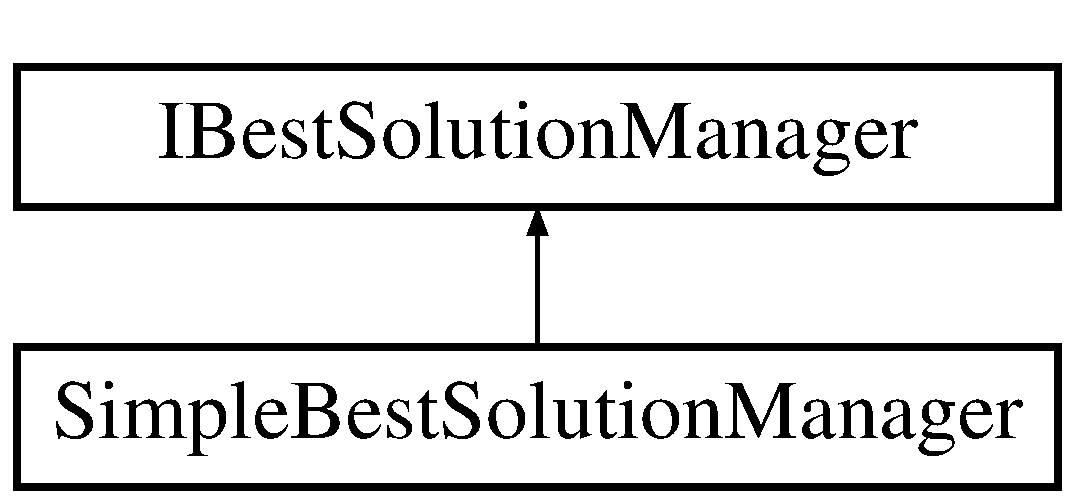
\includegraphics[height=2.000000cm]{classSimpleBestSolutionManager}
\end{center}
\end{figure}
\subsection*{\-Public \-Member \-Functions}
\begin{DoxyCompactItemize}
\item 
\hypertarget{classSimpleBestSolutionManager_a776c41f8abf2720ecbdfea78d88b0f00}{{\bfseries \-Simple\-Best\-Solution\-Manager} (\hyperlink{classALNS__Parameters}{\-A\-L\-N\-S\-\_\-\-Parameters} \&param)}\label{classSimpleBestSolutionManager_a776c41f8abf2720ecbdfea78d88b0f00}

\item 
virtual bool \hyperlink{classSimpleBestSolutionManager_a8237e1d633717d3dc69c35ff5a88497a}{is\-New\-Best\-Solution} (\hyperlink{classISolution}{\-I\-Solution} \&sol)
\item 
\hypertarget{classSimpleBestSolutionManager_a3dda02789fdfd353d0759567d5514977}{std\-::list$<$ \hyperlink{classISolution}{\-I\-Solution} $\ast$ $>$\-::iterator \hyperlink{classSimpleBestSolutionManager_a3dda02789fdfd353d0759567d5514977}{begin} ()}\label{classSimpleBestSolutionManager_a3dda02789fdfd353d0759567d5514977}

\begin{DoxyCompactList}\small\item\em \-Return a pointer to a best solution. \end{DoxyCompactList}\item 
\hypertarget{classSimpleBestSolutionManager_a1c8934fa905385e6ba6570e694101e29}{std\-::list$<$ \hyperlink{classISolution}{\-I\-Solution} $\ast$ $>$\-::iterator \hyperlink{classSimpleBestSolutionManager_a1c8934fa905385e6ba6570e694101e29}{end} ()}\label{classSimpleBestSolutionManager_a1c8934fa905385e6ba6570e694101e29}

\begin{DoxyCompactList}\small\item\em \-Return a pointer to a best solution. \end{DoxyCompactList}\item 
virtual \hyperlink{classISolution}{\-I\-Solution} $\ast$ \hyperlink{classSimpleBestSolutionManager_ab65e6cbfff67aa80bab7c05c4c07f7a1}{reload\-Best\-Solution} (\hyperlink{classISolution}{\-I\-Solution} $\ast$curr\-Sol, \hyperlink{classALNS__Iteration__Status}{\-A\-L\-N\-S\-\_\-\-Iteration\-\_\-\-Status} \&status)
\end{DoxyCompactItemize}


\subsection{\-Member \-Function \-Documentation}
\hypertarget{classSimpleBestSolutionManager_a8237e1d633717d3dc69c35ff5a88497a}{\index{\-Simple\-Best\-Solution\-Manager@{\-Simple\-Best\-Solution\-Manager}!is\-New\-Best\-Solution@{is\-New\-Best\-Solution}}
\index{is\-New\-Best\-Solution@{is\-New\-Best\-Solution}!SimpleBestSolutionManager@{\-Simple\-Best\-Solution\-Manager}}
\subsubsection[{is\-New\-Best\-Solution}]{\setlength{\rightskip}{0pt plus 5cm}bool {\bf \-Simple\-Best\-Solution\-Manager\-::is\-New\-Best\-Solution} (
\begin{DoxyParamCaption}
\item[{{\bf \-I\-Solution} \&}]{sol}
\end{DoxyParamCaption}
)\hspace{0.3cm}{\ttfamily  \mbox{[}virtual\mbox{]}}}}\label{classSimpleBestSolutionManager_a8237e1d633717d3dc69c35ff5a88497a}
\-This method evaluate if a solution is a new best solution, and adds it to the best solution pool in this case. 
\begin{DoxyParams}{\-Parameters}
{\em sol} & the solution to be tested. \\
\hline
\end{DoxyParams}
\begin{DoxyReturn}{\-Returns}
true if the solution is a new best solution, false otherwise. 
\end{DoxyReturn}


\-Implements \hyperlink{classIBestSolutionManager_adf056afba7bfda2b3a3260d8118d5c44}{\-I\-Best\-Solution\-Manager}.

\hypertarget{classSimpleBestSolutionManager_ab65e6cbfff67aa80bab7c05c4c07f7a1}{\index{\-Simple\-Best\-Solution\-Manager@{\-Simple\-Best\-Solution\-Manager}!reload\-Best\-Solution@{reload\-Best\-Solution}}
\index{reload\-Best\-Solution@{reload\-Best\-Solution}!SimpleBestSolutionManager@{\-Simple\-Best\-Solution\-Manager}}
\subsubsection[{reload\-Best\-Solution}]{\setlength{\rightskip}{0pt plus 5cm}{\bf \-I\-Solution} $\ast$ {\bf \-Simple\-Best\-Solution\-Manager\-::reload\-Best\-Solution} (
\begin{DoxyParamCaption}
\item[{{\bf \-I\-Solution} $\ast$}]{curr\-Sol, }
\item[{{\bf \-A\-L\-N\-S\-\_\-\-Iteration\-\_\-\-Status} \&}]{status}
\end{DoxyParamCaption}
)\hspace{0.3cm}{\ttfamily  \mbox{[}virtual\mbox{]}}}}\label{classSimpleBestSolutionManager_ab65e6cbfff67aa80bab7c05c4c07f7a1}
\-This function take care of reloading the best known solution, as the current solution, if needed. 
\begin{DoxyParams}{\-Parameters}
{\em curr\-Sol} & a pointer to the current solution. \\
\hline
{\em status} & the status of the current iteration. \\
\hline
\end{DoxyParams}
\begin{DoxyReturn}{\-Returns}
a pointer to the current solution. 
\end{DoxyReturn}


\-Implements \hyperlink{classIBestSolutionManager_a592e8c6de9b295e834ef04f52ae376a6}{\-I\-Best\-Solution\-Manager}.



\-The documentation for this class was generated from the following files\-:\begin{DoxyCompactItemize}
\item 
\-A\-L\-N\-S\-\_\-\-Static\-\_\-\-Lib/src/alns/\-Simple\-Best\-Solution\-Manager.\-h\item 
\-A\-L\-N\-S\-\_\-\-Static\-\_\-\-Lib/src/alns/\-Simple\-Best\-Solution\-Manager.\-cpp\end{DoxyCompactItemize}

\hypertarget{classSimpleLocalSearchManager}{\section{\-Simple\-Local\-Search\-Manager \-Class \-Reference}
\label{classSimpleLocalSearchManager}\index{\-Simple\-Local\-Search\-Manager@{\-Simple\-Local\-Search\-Manager}}
}
\-Inheritance diagram for \-Simple\-Local\-Search\-Manager\-:\begin{figure}[H]
\begin{center}
\leavevmode
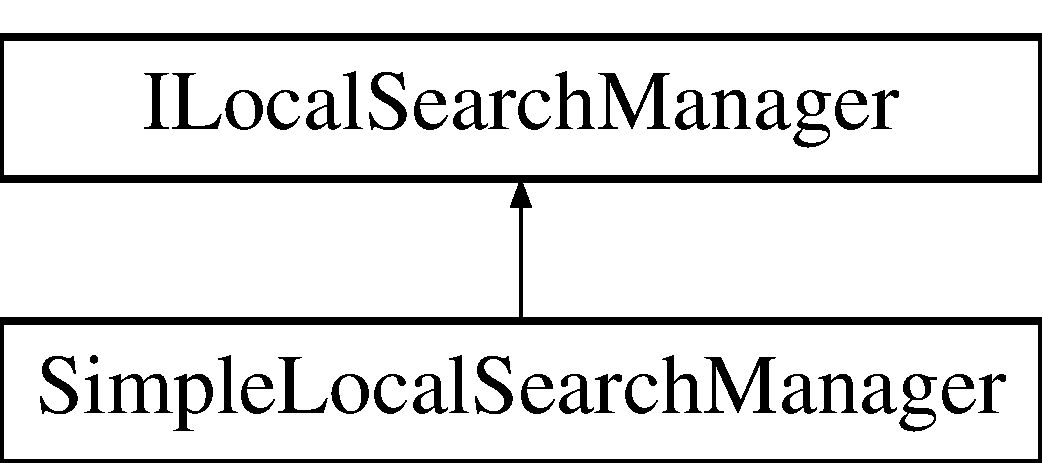
\includegraphics[height=2.000000cm]{classSimpleLocalSearchManager}
\end{center}
\end{figure}
\subsection*{\-Public \-Member \-Functions}
\begin{DoxyCompactItemize}
\item 
\hypertarget{classSimpleLocalSearchManager_a31e41079ea8d2aa1630bbee2f1cbe7fd}{{\bfseries \-Simple\-Local\-Search\-Manager} (\hyperlink{classALNS__Parameters}{\-A\-L\-N\-S\-\_\-\-Parameters} \&parameters)}\label{classSimpleLocalSearchManager_a31e41079ea8d2aa1630bbee2f1cbe7fd}

\item 
virtual bool \hyperlink{classSimpleLocalSearchManager_a213c380b351e4c7c4b4948ad7da513a7}{use\-Local\-Search} (\hyperlink{classISolution}{\-I\-Solution} \&sol, \hyperlink{classALNS__Iteration__Status}{\-A\-L\-N\-S\-\_\-\-Iteration\-\_\-\-Status} \&status)
\item 
\hypertarget{classSimpleLocalSearchManager_acd75ce5f7619a645520b5e1ebe854ee3}{void \hyperlink{classSimpleLocalSearchManager_acd75ce5f7619a645520b5e1ebe854ee3}{add\-Local\-Search\-Operator} (\hyperlink{classILocalSearch}{\-I\-Local\-Search} \&ls)}\label{classSimpleLocalSearchManager_acd75ce5f7619a645520b5e1ebe854ee3}

\begin{DoxyCompactList}\small\item\em \-Add a local search operator to the manager. \end{DoxyCompactList}\item 
\hypertarget{classSimpleLocalSearchManager_abf69f94e9d32260cf5eaed192c42114c}{virtual void \hyperlink{classSimpleLocalSearchManager_abf69f94e9d32260cf5eaed192c42114c}{start\-Signal} ()}\label{classSimpleLocalSearchManager_abf69f94e9d32260cf5eaed192c42114c}

\begin{DoxyCompactList}\small\item\em \-Indicate that the optimization process starts. \end{DoxyCompactList}\end{DoxyCompactItemize}


\subsection{\-Member \-Function \-Documentation}
\hypertarget{classSimpleLocalSearchManager_a213c380b351e4c7c4b4948ad7da513a7}{\index{\-Simple\-Local\-Search\-Manager@{\-Simple\-Local\-Search\-Manager}!use\-Local\-Search@{use\-Local\-Search}}
\index{use\-Local\-Search@{use\-Local\-Search}!SimpleLocalSearchManager@{\-Simple\-Local\-Search\-Manager}}
\subsubsection[{use\-Local\-Search}]{\setlength{\rightskip}{0pt plus 5cm}bool {\bf \-Simple\-Local\-Search\-Manager\-::use\-Local\-Search} (
\begin{DoxyParamCaption}
\item[{{\bf \-I\-Solution} \&}]{sol, }
\item[{{\bf \-A\-L\-N\-S\-\_\-\-Iteration\-\_\-\-Status} \&}]{status}
\end{DoxyParamCaption}
)\hspace{0.3cm}{\ttfamily  \mbox{[}virtual\mbox{]}}}}\label{classSimpleLocalSearchManager_a213c380b351e4c7c4b4948ad7da513a7}

\begin{DoxyParams}{\-Parameters}
{\em sol} & the solution to be improved. \\
\hline
{\em status} & the status of the alns iteration. \\
\hline
\end{DoxyParams}
\begin{DoxyReturn}{\-Returns}
true if the solution has been improved. 
\end{DoxyReturn}


\-Implements \hyperlink{classILocalSearchManager_ab12f478c7be7163b674374ba478f2cbd}{\-I\-Local\-Search\-Manager}.



\-The documentation for this class was generated from the following files\-:\begin{DoxyCompactItemize}
\item 
\-A\-L\-N\-S\-\_\-\-Static\-\_\-\-Lib/src/localsearch/\-Simple\-Local\-Search\-Manager.\-h\item 
\-A\-L\-N\-S\-\_\-\-Static\-\_\-\-Lib/src/localsearch/\-Simple\-Local\-Search\-Manager.\-cpp\end{DoxyCompactItemize}

\hypertarget{classSimulatedAnnealing}{\section{\-Simulated\-Annealing \-Class \-Reference}
\label{classSimulatedAnnealing}\index{\-Simulated\-Annealing@{\-Simulated\-Annealing}}
}


\-Use a simulated annealing principle to decide whether or not a new solution should be accepted as the current solution.  




{\ttfamily \#include $<$\-Simulated\-Annealing.\-h$>$}

\-Inheritance diagram for \-Simulated\-Annealing\-:\begin{figure}[H]
\begin{center}
\leavevmode
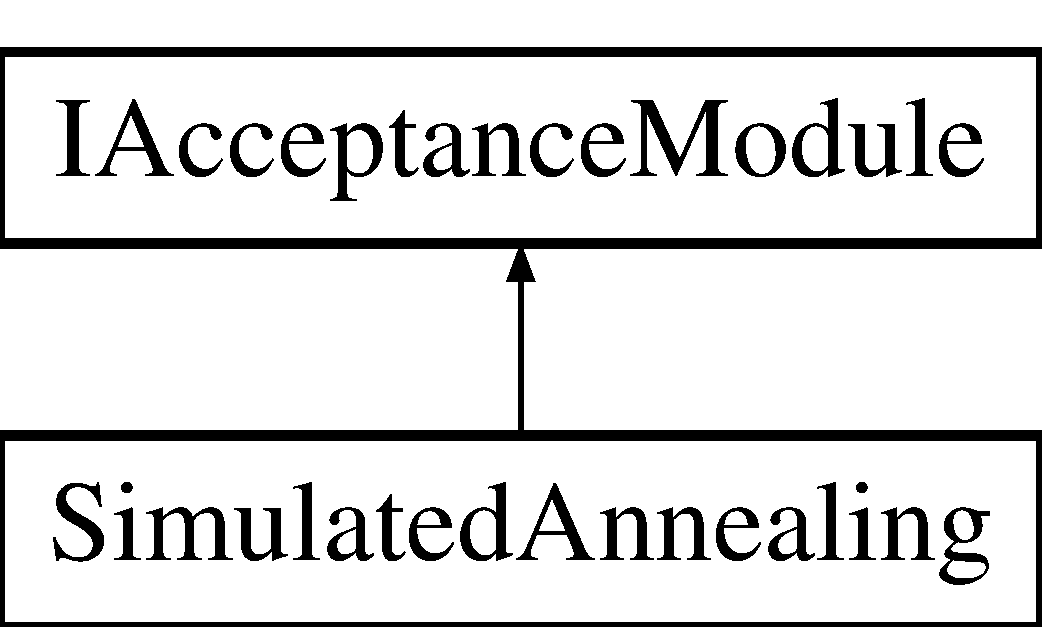
\includegraphics[height=2.000000cm]{classSimulatedAnnealing}
\end{center}
\end{figure}
\subsection*{\-Public \-Member \-Functions}
\begin{DoxyCompactItemize}
\item 
\hyperlink{classSimulatedAnnealing_ab8106a8cd0e1e6ec82e6e74a27639308}{\-Simulated\-Annealing} (\hyperlink{classICoolingSchedule}{\-I\-Cooling\-Schedule} \&cs)
\item 
\hypertarget{classSimulatedAnnealing_ab8630a5a98e257bab37f9b998329e397}{virtual \hyperlink{classSimulatedAnnealing_ab8630a5a98e257bab37f9b998329e397}{$\sim$\-Simulated\-Annealing} ()}\label{classSimulatedAnnealing_ab8630a5a98e257bab37f9b998329e397}

\begin{DoxyCompactList}\small\item\em \-Destructor. \end{DoxyCompactList}\item 
\hypertarget{classSimulatedAnnealing_a1bea2151b5c2b9b18f16bb47337af3cc}{bool \hyperlink{classSimulatedAnnealing_a1bea2151b5c2b9b18f16bb47337af3cc}{transition\-Accepted} (\hyperlink{classIBestSolutionManager}{\-I\-Best\-Solution\-Manager} \&best\-Solution\-Manager, \hyperlink{classISolution}{\-I\-Solution} \&current\-Solution, \hyperlink{classISolution}{\-I\-Solution} \&new\-Solution, \hyperlink{classALNS__Iteration__Status}{\-A\-L\-N\-S\-\_\-\-Iteration\-\_\-\-Status} \&status)}\label{classSimulatedAnnealing_a1bea2151b5c2b9b18f16bb47337af3cc}

\begin{DoxyCompactList}\small\item\em \-Compute if the newly created solution have to be accepted or not. \end{DoxyCompactList}\item 
virtual void \hyperlink{classSimulatedAnnealing_a13ddd574a0528f64801016a235ec8ee3}{start\-Signal} ()
\end{DoxyCompactItemize}


\subsection{\-Detailed \-Description}
\-Use a simulated annealing principle to decide whether or not a new solution should be accepted as the current solution. 

\-If you are interested by simulated annealing, please refer to\-: \-Kirkpatrick, \-S.; \-Gelatt, \-C. \-D.; \-Vecchi, \-M. \-P. (1983). \char`\"{}\-Optimization by Simulated
 Annealing\char`\"{}. \-Science 220 (4598)\-: 671–680 or \href{http://en.wikipedia.org/wiki/Simulated_annealing}{\tt http\-://en.\-wikipedia.\-org/wiki/\-Simulated\-\_\-annealing} 

\subsection{\-Constructor \& \-Destructor \-Documentation}
\hypertarget{classSimulatedAnnealing_ab8106a8cd0e1e6ec82e6e74a27639308}{\index{\-Simulated\-Annealing@{\-Simulated\-Annealing}!\-Simulated\-Annealing@{\-Simulated\-Annealing}}
\index{\-Simulated\-Annealing@{\-Simulated\-Annealing}!SimulatedAnnealing@{\-Simulated\-Annealing}}
\subsubsection[{\-Simulated\-Annealing}]{\setlength{\rightskip}{0pt plus 5cm}{\bf \-Simulated\-Annealing\-::\-Simulated\-Annealing} (
\begin{DoxyParamCaption}
\item[{{\bf \-I\-Cooling\-Schedule} \&}]{cs}
\end{DoxyParamCaption}
)}}\label{classSimulatedAnnealing_ab8106a8cd0e1e6ec82e6e74a27639308}
\-Constructor. 
\begin{DoxyParams}{\-Parameters}
{\em cs} & the cooling schedule to be used by the simulated annealing. \\
\hline
\end{DoxyParams}


\subsection{\-Member \-Function \-Documentation}
\hypertarget{classSimulatedAnnealing_a13ddd574a0528f64801016a235ec8ee3}{\index{\-Simulated\-Annealing@{\-Simulated\-Annealing}!start\-Signal@{start\-Signal}}
\index{start\-Signal@{start\-Signal}!SimulatedAnnealing@{\-Simulated\-Annealing}}
\subsubsection[{start\-Signal}]{\setlength{\rightskip}{0pt plus 5cm}void {\bf \-Simulated\-Annealing\-::start\-Signal} (
\begin{DoxyParamCaption}
{}
\end{DoxyParamCaption}
)\hspace{0.3cm}{\ttfamily  \mbox{[}virtual\mbox{]}}}}\label{classSimulatedAnnealing_a13ddd574a0528f64801016a235ec8ee3}
\-Some \-Acceptance modules needs to initialize some variable only when the solver actualy starts working. \-In this case you should override this method. 

\-Reimplemented from \hyperlink{classIAcceptanceModule_adf6b1054982d528815e339aa8a829d4a}{\-I\-Acceptance\-Module}.



\-The documentation for this class was generated from the following files\-:\begin{DoxyCompactItemize}
\item 
\-A\-L\-N\-S\-\_\-\-Static\-\_\-\-Lib/src/acceptance\-Module/\-Simulated\-Annealing.\-h\item 
\-A\-L\-N\-S\-\_\-\-Static\-\_\-\-Lib/src/acceptance\-Module/\-Simulated\-Annealing.\-cpp\end{DoxyCompactItemize}

\hypertarget{classStatistics}{\section{\-Statistics \-Class \-Reference}
\label{classStatistics}\index{\-Statistics@{\-Statistics}}
}
\subsection*{\-Public \-Member \-Functions}
\begin{DoxyCompactItemize}
\item 
\hypertarget{classStatistics_a60ddd90a571ed4c3ce8c0f6317a36d63}{\hyperlink{classStatistics_a60ddd90a571ed4c3ce8c0f6317a36d63}{\-Statistics} ()}\label{classStatistics_a60ddd90a571ed4c3ce8c0f6317a36d63}

\begin{DoxyCompactList}\small\item\em \-Constructor. \end{DoxyCompactList}\item 
\hypertarget{classStatistics_ab68ede75479e44d5c35b78ec1284065b}{virtual \hyperlink{classStatistics_ab68ede75479e44d5c35b78ec1284065b}{$\sim$\-Statistics} ()}\label{classStatistics_ab68ede75479e44d5c35b78ec1284065b}

\begin{DoxyCompactList}\small\item\em \-Destructor. \end{DoxyCompactList}\item 
\hypertarget{classStatistics_a3f0fd8c2da757960f26749fc1394d01e}{void \hyperlink{classStatistics_a3f0fd8c2da757960f26749fc1394d01e}{add\-Entry} (double time\-Stamp, size\-\_\-t iteration, std\-::string destroy\-Name, std\-::string recreate\-Name, double new\-Cost, double current\-Cost, double best\-Cost, int cum\-K\-S)}\label{classStatistics_a3f0fd8c2da757960f26749fc1394d01e}

\begin{DoxyCompactList}\small\item\em \-This method adds an entry to the data. \end{DoxyCompactList}\item 
\hypertarget{classStatistics_a5fc6621a8e83fcd2eb4b8d8597e60177}{void {\bfseries add\-Operator\-Entry} (std\-::vector$<$ double $>$ $\ast$weight, std\-::vector$<$ size\-\_\-t $>$ $\ast$calls)}\label{classStatistics_a5fc6621a8e83fcd2eb4b8d8597e60177}

\item 
\hypertarget{classStatistics_a42db1ff91fa1657d4d61412b18111695}{void {\bfseries add\-Operators\-Names} (std\-::vector$<$ std\-::string $>$ $\ast$names)}\label{classStatistics_a42db1ff91fa1657d4d61412b18111695}

\item 
\hypertarget{classStatistics_ab02409562fa0f74d240356b7fc4a35d7}{void \hyperlink{classStatistics_ab02409562fa0f74d240356b7fc4a35d7}{generate\-Stats\-File} (std\-::string path, std\-::string path\-Op)}\label{classStatistics_ab02409562fa0f74d240356b7fc4a35d7}

\begin{DoxyCompactList}\small\item\em \-This method generate the file containing the datas. \end{DoxyCompactList}\item 
\hypertarget{classStatistics_af2593852c918bd4110c2ec649b146537}{void {\bfseries set\-Start} ()}\label{classStatistics_af2593852c918bd4110c2ec649b146537}

\end{DoxyCompactItemize}


\-The documentation for this class was generated from the following files\-:\begin{DoxyCompactItemize}
\item 
\-A\-L\-N\-S\-\_\-\-Static\-\_\-\-Lib/src/statistics/\-Statistics.\-h\item 
\-A\-L\-N\-S\-\_\-\-Static\-\_\-\-Lib/src/statistics/\-Statistics.\-cpp\end{DoxyCompactItemize}

\hypertarget{classTimeLinearCoolingSchedule}{\section{\-Time\-Linear\-Cooling\-Schedule \-Class \-Reference}
\label{classTimeLinearCoolingSchedule}\index{\-Time\-Linear\-Cooling\-Schedule@{\-Time\-Linear\-Cooling\-Schedule}}
}


\-A linear cooling schedule based on the maximum running time.  




{\ttfamily \#include $<$\-Time\-Linear\-Cooling\-Schedule.\-h$>$}

\-Inheritance diagram for \-Time\-Linear\-Cooling\-Schedule\-:\begin{figure}[H]
\begin{center}
\leavevmode
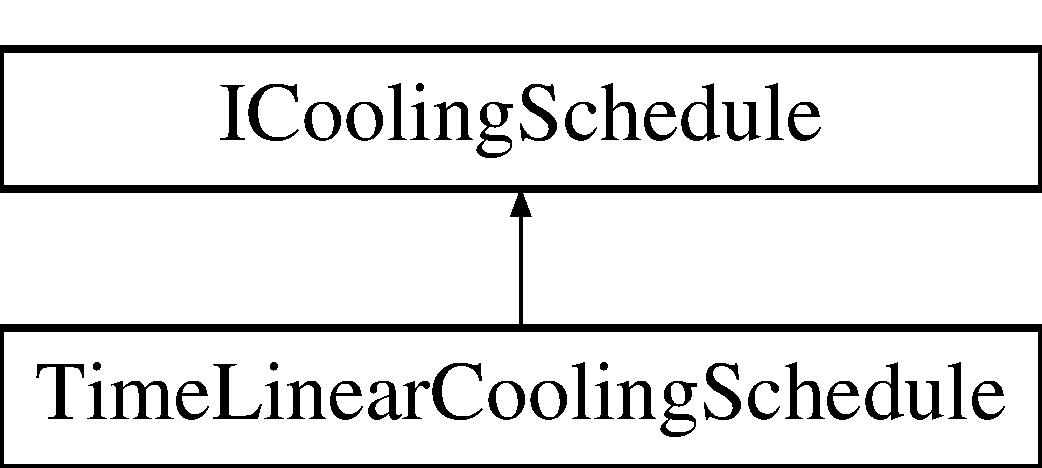
\includegraphics[height=2.000000cm]{classTimeLinearCoolingSchedule}
\end{center}
\end{figure}
\subsection*{\-Public \-Member \-Functions}
\begin{DoxyCompactItemize}
\item 
\hyperlink{classTimeLinearCoolingSchedule_ab5fa018fab6d1fb011e6e91bfdb6641a}{\-Time\-Linear\-Cooling\-Schedule} (\hyperlink{classISolution}{\-I\-Solution} \&init\-Sol, \hyperlink{classCoolingSchedule__Parameters}{\-Cooling\-Schedule\-\_\-\-Parameters} \&cs\-Param)
\item 
\hypertarget{classTimeLinearCoolingSchedule_a0877911daae13d58c67a2a6b7c384397}{virtual \hyperlink{classTimeLinearCoolingSchedule_a0877911daae13d58c67a2a6b7c384397}{$\sim$\-Time\-Linear\-Cooling\-Schedule} ()}\label{classTimeLinearCoolingSchedule_a0877911daae13d58c67a2a6b7c384397}

\begin{DoxyCompactList}\small\item\em \-Destructor. \end{DoxyCompactList}\item 
double \hyperlink{classTimeLinearCoolingSchedule_a67dffb918e6c67ba8fecad1b764f36ea}{get\-Current\-Temperature} ()
\item 
virtual void \hyperlink{classTimeLinearCoolingSchedule_a44190e4c27b218610724a8e41c65291f}{start\-Signal} ()
\end{DoxyCompactItemize}


\subsection{\-Detailed \-Description}
\-A linear cooling schedule based on the maximum running time. 

\subsection{\-Constructor \& \-Destructor \-Documentation}
\hypertarget{classTimeLinearCoolingSchedule_ab5fa018fab6d1fb011e6e91bfdb6641a}{\index{\-Time\-Linear\-Cooling\-Schedule@{\-Time\-Linear\-Cooling\-Schedule}!\-Time\-Linear\-Cooling\-Schedule@{\-Time\-Linear\-Cooling\-Schedule}}
\index{\-Time\-Linear\-Cooling\-Schedule@{\-Time\-Linear\-Cooling\-Schedule}!TimeLinearCoolingSchedule@{\-Time\-Linear\-Cooling\-Schedule}}
\subsubsection[{\-Time\-Linear\-Cooling\-Schedule}]{\setlength{\rightskip}{0pt plus 5cm}{\bf \-Time\-Linear\-Cooling\-Schedule\-::\-Time\-Linear\-Cooling\-Schedule} (
\begin{DoxyParamCaption}
\item[{{\bf \-I\-Solution} \&}]{init\-Sol, }
\item[{{\bf \-Cooling\-Schedule\-\_\-\-Parameters} \&}]{cs\-Param}
\end{DoxyParamCaption}
)}}\label{classTimeLinearCoolingSchedule_ab5fa018fab6d1fb011e6e91bfdb6641a}
\-Constructor. 
\begin{DoxyParams}{\-Parameters}
{\em init\-Sol} & the initial solution. \\
\hline
{\em cs\-Param} & the cooling schedule parameters to be used. \\
\hline
\end{DoxyParams}


\subsection{\-Member \-Function \-Documentation}
\hypertarget{classTimeLinearCoolingSchedule_a67dffb918e6c67ba8fecad1b764f36ea}{\index{\-Time\-Linear\-Cooling\-Schedule@{\-Time\-Linear\-Cooling\-Schedule}!get\-Current\-Temperature@{get\-Current\-Temperature}}
\index{get\-Current\-Temperature@{get\-Current\-Temperature}!TimeLinearCoolingSchedule@{\-Time\-Linear\-Cooling\-Schedule}}
\subsubsection[{get\-Current\-Temperature}]{\setlength{\rightskip}{0pt plus 5cm}double {\bf \-Time\-Linear\-Cooling\-Schedule\-::get\-Current\-Temperature} (
\begin{DoxyParamCaption}
{}
\end{DoxyParamCaption}
)\hspace{0.3cm}{\ttfamily  \mbox{[}virtual\mbox{]}}}}\label{classTimeLinearCoolingSchedule_a67dffb918e6c67ba8fecad1b764f36ea}
\-Compute and return the current temperature. \begin{DoxyReturn}{\-Returns}
the current temperature. 
\end{DoxyReturn}


\-Implements \hyperlink{classICoolingSchedule_ac5d2dbf784cde3a36fd5e7c5c3fbdd96}{\-I\-Cooling\-Schedule}.

\hypertarget{classTimeLinearCoolingSchedule_a44190e4c27b218610724a8e41c65291f}{\index{\-Time\-Linear\-Cooling\-Schedule@{\-Time\-Linear\-Cooling\-Schedule}!start\-Signal@{start\-Signal}}
\index{start\-Signal@{start\-Signal}!TimeLinearCoolingSchedule@{\-Time\-Linear\-Cooling\-Schedule}}
\subsubsection[{start\-Signal}]{\setlength{\rightskip}{0pt plus 5cm}void {\bf \-Time\-Linear\-Cooling\-Schedule\-::start\-Signal} (
\begin{DoxyParamCaption}
{}
\end{DoxyParamCaption}
)\hspace{0.3cm}{\ttfamily  \mbox{[}virtual\mbox{]}}}}\label{classTimeLinearCoolingSchedule_a44190e4c27b218610724a8e41c65291f}
\-This method should be called when the optimization process start. \-The cooling schedules that actually need this should override this method. 

\-Reimplemented from \hyperlink{classICoolingSchedule_aa87b9fe07eb7f03a7c4bad8f6f31b8a2}{\-I\-Cooling\-Schedule}.



\-The documentation for this class was generated from the following files\-:\begin{DoxyCompactItemize}
\item 
\-A\-L\-N\-S\-\_\-\-Static\-\_\-\-Lib/src/acceptance\-Module/\-Time\-Linear\-Cooling\-Schedule.\-h\item 
\-A\-L\-N\-S\-\_\-\-Static\-\_\-\-Lib/src/acceptance\-Module/\-Time\-Linear\-Cooling\-Schedule.\-cpp\end{DoxyCompactItemize}

\printindex
\end{document}
